\chapter{Evaluation}
Um Ergebnisse zu den verschiedenen Methodiken zu erhalten wird ihre jeweile Verwendung zu esrt simuliert und die so erhaltenen Ergebnisse anschließend analysiert und verglichen.
\section{Simulationsaufbau}
Zunächst wird auf den Aufbau des verwendeten Simulators eingegangen, sowie auf die ,in der Simulationen verwendeten, Daten.
\subsection{Simulationsframework und Simulatoren}
Für die Durchführung der Simulation der in Kapitel \ref{chap_Body} vorgestellten Methodiken wird die Co-Simulation Software Mosaik \footnote{https://mosaik.offis.de/}, in Version 2.5.1, verwendet. Der Mosiak Simulator wurde speziell für Simulation von Smart Grid-Anwendung entwickelt und eignet sich deswegen hervorragend für die im Zuge dieser Arbeit zu erfüllenden Aufgaben. Der Simulator unterstützt zudem die schnelle Einbindung von einem Framework namens PYPOWER. PYPOWER wurde zur Simulation von Stromflüssen entwickelt und ist in der Lage anhand eines Stromnetzes die Ströme der elektrischen Energie zu simulieren. Diese Simulation des Stromflusses schließt auch den Transportverlust der Niederspannung und den Zusammenhang von Wirk- zu Blindleistung mit ein. PyPower wird hier in der Version 5.1.4 verwendet. Mosaik verbindet drei verschieden Simulatoren miteinander, welche das Stromnetz, die Elektrofahrzeuge und den aktuell verwendeten Kontroller darstellen.
Das Stromnetz, welches in dieser Arbeit verwendet wird, ist ein standardisiertes europäisches Niederspannungsnetz.  Dieses wurde von der IEEE, dem Institut für Elektro- und Elektronikingenieure, für solche Simulationen herausgegeben, um Ergebnisse auf einer EU-weiten Ebene vergleichbarer zu machen. Das IEEE906 Netz beinhalten minutenweise gestaffelte Daten, welche die Grundlast der 55 verfügbaren Haushalte darstellen. Das Stromnetz liegt in Form eines mosaik-pypower Simulators vor, dieser Simulator wurde nicht im Zuge dieser Arbeit entwickelt, sondern er wird nur verwendet. Der Netzsimulator benötigt beim Starten die Startzeit der Simulation, um Zeit der Simulation zu synchronisieren. In jedem Zeitintervall ist jedem Anschlusspunkt die dort aktuelle Spannung bekannt und kann so von den Verbrauchern verwendet werden und die Verbraucher können die Höhe der über diesen Anschlusspunkt bezogenen Leistung dem Anschlusspunkt übergeben.
Die Daten der Elektrofahrzeuge sind ebenfalls in einem Simulator enthalten, welcher mit Mosaik verwendet wird. Die Daten der Elektrofahrzeuge werden über den FlexEV Simulator zur Verfügung gestellt, von welchem die Version 1.1.4 verwendet wurde. Beim Starten des Simulators wird die aktuelle Startzeit, zur Synchronisation der Zeit, übergeben. Die einzelnen Elektrofahrzeuge erhalten Information an welchem Anschlusspunkt des Niederspannungsnetzes sie angeschlossen sind, die maximal mögliche Stromstärke beim Laden, sowie die verwendete Batteriekapazität. Der Simulator stellt in Minuten Intervallen gestaffelte Daten zu den einzelnen Elektrofahrzeugen zur Verfügung. Diese Daten bestehen aus dem Ankunftszeitpunkt, dem Abfahrtszeitpunkt, dem Ladezustand der Batterie, der aktuell möglichen Stromstärke beim Laden sowie einem Indikator, ob sich das Fahrzeug aktuell an einem Ladegerät befindet. Die mögliche Ladeleistung eines jeden Elektrofahrzeuges wird individuell vom dazugehörigen Kontroller bestimmt und dem Elektrofahrzeug übergeben. Diese Leistung wird dann vom Elektrofahrzeug an den entsprechenden Anschlusspunkt übergeben, nachdem der Wirkungsgrad des Ladegeräts berücksichtig wird.
Die einzelnen Kontroller sind ebenfalls einem Simulator enthalten. Dieser Simulator benötigt beim Start die Länge eines Zeitschrittes, sowie die aktuell verwendete Methodik. Jeder Kontroller ist mit einem Elektrofahrzeug sowie einem Anschlusspunkt ans Netz verknüpft. Jeder Kontroller erhält die Daten die diese beiden bereitstellen, die aktuelle Spannung, die Ankunfts- und Abfahrtszeit, den Ladezustand der Batterie, die aktuell möglichen Stromstärke beim Laden sowie einem Indikator, ob sich das Fahrzeug aktuell an einem Ladegerät befindet. Anhand dieser Daten bestimmt der Kontroller ausgehend von der verwendeten Methodik die mögliche Ladeleistung des Elektrofahrzeuges und übergibt diesen Wert an das Fahrzeug. Der Kontroller erhält weitere Daten, die Transformatorlast, sowie die Anzahl der aktuellen Teilnehmer, über ein impliziert implementiertes Broadcastsystem, welches keine Eigenschaften der Kommunikation, wie Verzögerungen oder Paketverluste, simuliert. 
\begin{figure}[htb]
\centering
	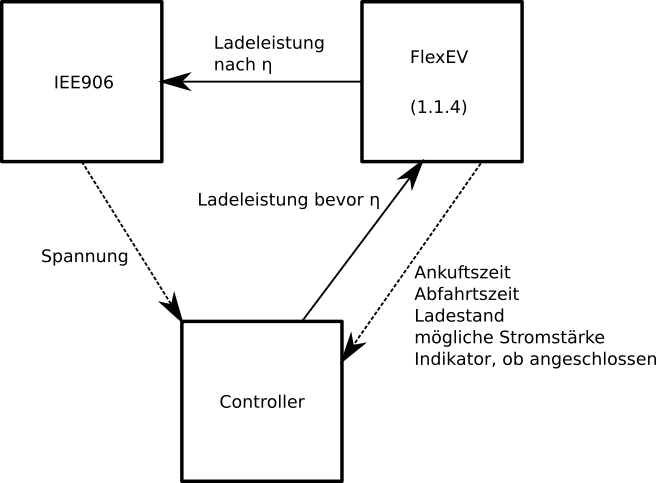
\includegraphics[width=0.5\textwidth]{img/SimAufbau3.png}
	\caption{Schnittstellen zwischen den Teilen des Simulators}
	\label{Abb_SimAufbau}
\end{figure}

In der Abbildung \ref{Abb_SimAufbau} wird verdeutlicht, welche Daten die Simulatoren an andere Simulatoren übergeben. Den beiden gestrichelten Pfeilen kommt eine Sonderrolle zu. Diese Sonderrolle sieht vor das Daten zeitlich verschoben, bereits zu Beginn des Zeitschrittes, zur Verfügung gestellt werden, um Deadlocks zwischen den Simulatoren zu verhindern. Ein solcher Deadlock kann auftreten, wenn Simulatoren auf Daten anderer Simulatoren warten, welche aber ebenfalls auf Daten warten. Ein solcher Deadlock kann immer dann entstehen, wenn Zyklen in den Beziehungen der Teilnehmer vorhanden sind. \\
\begin{table}[tbh]
\centering
\begin{tabular}{|l|l|}
\hline
Bibliotek           & Version    \\ \hline \hline
datetime            & 3.8        \\ \hline
math                & 3.8        \\ \hline
mosaik              & 2.5.1      \\ \hline
mosaik-api          & 2.4        \\ \hline
random              & 3.8        \\ \hline
socket              & 3.8        \\ \hline
\end{tabular}
\caption{Verwendete Python Bibliotheken mit der jeweiligen verwendeten Version}
\label{tab:my-tableLib}
\end{table}

Tabelle \ref{tab:my-tableLib} listet in den Simulationen verwendete Bibliotheken mit der entsprechenden Versionsnummer auf. Die Bibliotheken bringen zusätzliche Funktionalität ein, welche für die Durchführung der Simulationen benötigt wird, aber nicht von vorn herein Bestandteil des verwendeten Systems ist.  
\subsection{Annahmen und verwendete Daten}
Im Zuge dieser Arbeit werden auch Daten verarbeitet. Die Mehrheit dieser Daten steht in Zusammenhang mit den Elektrofahrzeugen. Die Daten die diese für die Simulation zur Verfügung stellen, wurden im Auftrag des Bundesministerium für Verkehr und digitale Infrastruktur erhoben \footnote{http://mobilitaetspanel.ifv.kit.edu/beteiligte.php}. Diese Erhebung fand im Zuge einer Mobilitätsstudie statt. Es wurden Teilnehmer für diese Studie aus der Bevölkerung ausgewählt, welche dann ihr Mobilitätsverhalten dokumentiert haben. Diese Mobilitätsverhalten dienen als Grundlage für die Daten der verwendeten Elektrofahrzeuge. Durch die Auswertung dieser Daten wurden Ankunfts- und Abfahrtszeiten, sowie die jeweils gefahrene Wegstrecke bestimmt. Durch die Länge der Wegstrecke kann bestimmt werden wie viel des Ladezustandes auf dieser Strecke verbraucht wird und somit auch der Ladestand bei Ankunft an der Ladestation.\\
Es werden für die Simulationen auch einige Annahmen getroffen. Die mittlere Kapazität der Batterie, in welcher die elektrische Energie der Elektrofahrzeuge gespeichert wird, wird auf 36253,11 Wh festgelegt. Dieser Wert durch die Kombination zweier Datensätze ermittelt. Der erste dieser Datensätze enthält die Zulassungszahlen von elektrisch angetrieben Fahrzeugen in Deutschland von den Jahren 2013 bis 2019(\cite{ahlswede_2020}), betrachtet wurde jedoch nur der Zeitraum bis 2018. Der zweite Datensatz enthält die Kapazitäten der in Elektrofahrzeugen verbauten Batterien (\cite{akkuStat}). Durch die Verwendung dieser Statistiken wurde die durchschnittliche Batteriekapazität eines in Deutschland zugelassenen Elektrofahrzeuges ermittelt. Dieser Mittelwert stellt einen Kompromiss zu einer individuellen Batteriekapazität dar, stellt allerdings auch sicher vergleichbare Ergebnisse zu erhalten. Die Norm DIN EN 50160 setzt die Normspannung im Deutschem Stromnetz auf 230 Volt, daher wird dieser auch in dieser Arbeit verwendet. Die maximale Trafolast wurde durch eine Simulation ohne Aktivität von Elektrofahrzeugen ermittelt. Die, in dieser Simulation gemessene, Transformatorlast wurde verdoppelt. Diese Verdopplung soll die Belastung des Transformators so gering wie möglich halten, den Ladevorgängen aber dennoch die Möglichkeit bieten auch Leistung abzurufen. Eine Verdopplung sorgt außerdem dafür, die beim der Planung des Netzes einkalkulierten Reserven, welche nicht nur der Ausfallsicherheit dieses Netzes sondern auch der umliegenden dient, zu erhalten und so auch auch noch in Ausnahmesituationen den Betrieb gewährleisten zu können.\\
Eine weitere Annahme ist die maximale Anzahl an Elektrofahrzeugen, hierbei wurde davon ausgegangen, dass ein jeder Haushalt im Niederspannungsnetz über exakt zwei Elektrofahrzeuge verfügt, welche mithilfe eine 22kW Ladegeräts geladen werden. Diese Annahme geht aus Statistiken eines Bundesamtes(\cite{hochstetter_2015}) zurück, welche aussagt, das in ländlich geprägten Gebieten vermehrt größere Haushaltemit zwei oder mehr Personen auftreten. Aus Gründen der Normalisierung zwischen den Anschlusspunkten ans Niederspannungsnetz, wird daher immer von zwei Fahrzeugen je Anschlusspunkt ausgegangen. Das hierverwendet Stromnetz, IEEE906, verfügt über 55 Anschlusspunkte für Privathaushalte, folglich wird in den Simulationen von 110 Elektrofahrzeugen ausgegangen.\\

\section{Simulationsergebnisse}
Die Ergebnisse der durchlaufenen Simulationen werden zunächst aufgeteilt auf die verschiedenen Methodiken vorgestellt. Die verschiedenen Methodiken wurden über den Zeitraum von einer Woche hinweg simuliert. Bei der Darstellung der Transformatorlast, der Spannungswerte und der Teilnehmerzahlen werden jeweils nur die Ergebnisse eines einzelnen Werktages dargestellt, um eine bessere Übersichtlichkeit der Graphen zu erreichen. Ein Werktag wurde gewählt, da eine Woche aus mehr Werktage als anderen Tagen besteht und die Ergebnisse so repräsentativer sind. \\
In den einzelnen Analysen wird jeweils auf die Transformatorlast, die Spannungswerte, die ladebereiten und ladeneden Teilnehmer, die Spannungsqualität, die Anzahl an Kollisionen, den Ladestand über den Verlauf der Ladeservice, sowie auf die Qualitätserfahrung und die Fairness eingegangen. Die Methoden SA+T, SA+T+F, SA+T+Tr und SA+T+F+Tr verwenden ein Intervall, aus welchem eine Zufallszahl gezogen wird, um die Wartezeit nach einer Kollision zu bestimmen. Für die Bestimmung dieser Zufallszahlen wurden verschiedene Startwerte verwendet, um den Einfluss der einzelnen Startwerte durch Bildung von Mittelwerten, über die erhaltenen Ergebnisse, auszugleichen zu können. Die Simulationen dieser vier Methodiken wurden mit 10 unterschiedlichen Startwerten ausgeführt. Die für diese Methodiken angegebenen Ergebnisse sind die Mittelwerte samt Standardabweichung dieser Durchläufe.
\subsection{VDE-Controller}
\label{chap_VDE}
Als Erstes werden die Ergebnisse bei der Verwendung des VDE-Kontrollers vorgestellt.
\begin{figure}
\begin{subfigure}{\linewidth}
	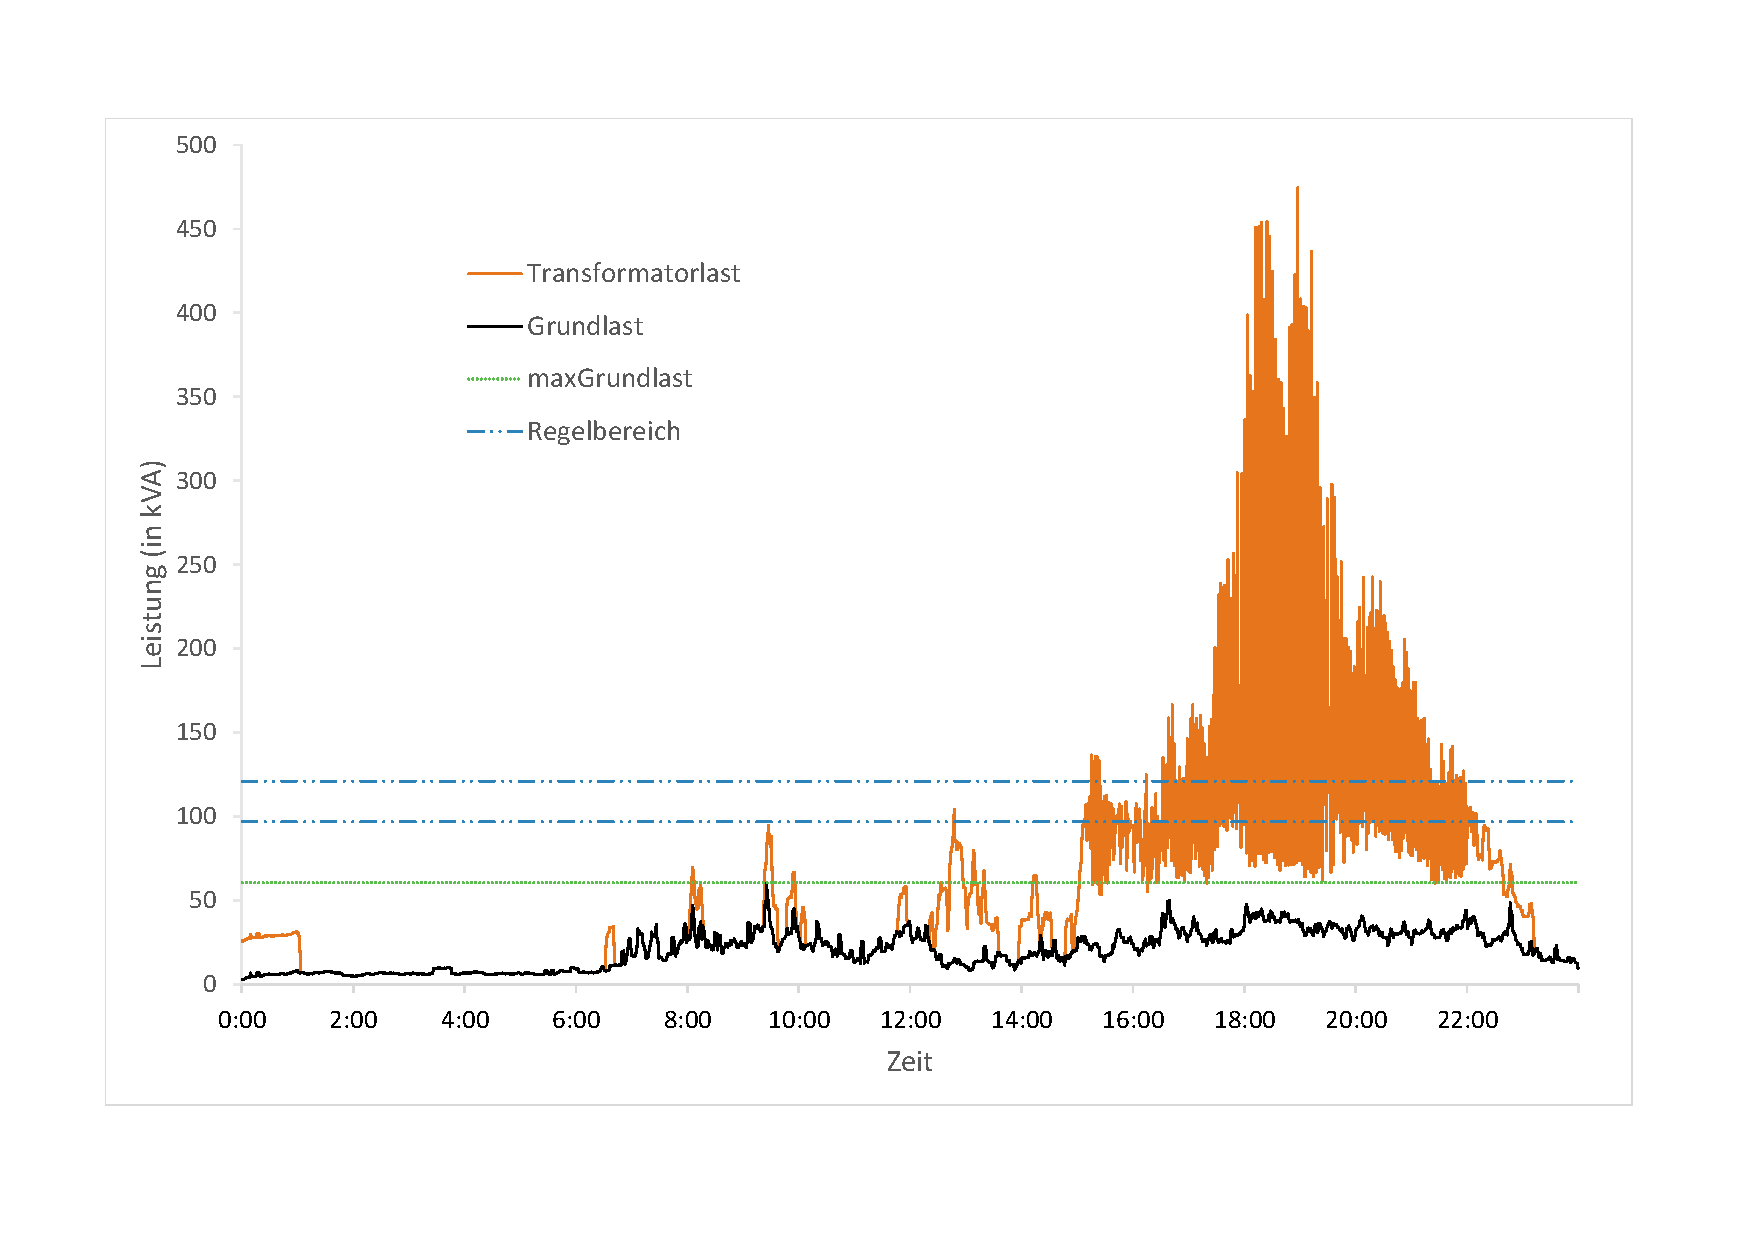
\includegraphics[scale=0.45]{img/VDE_tau/TrafoLast9.pdf}
	\caption{Transformatorlast über den Verlauf eines Tages}
	\label{Abb_VDEtauTrafoLast}
\end{subfigure}
\begin{subfigure}{\linewidth}
	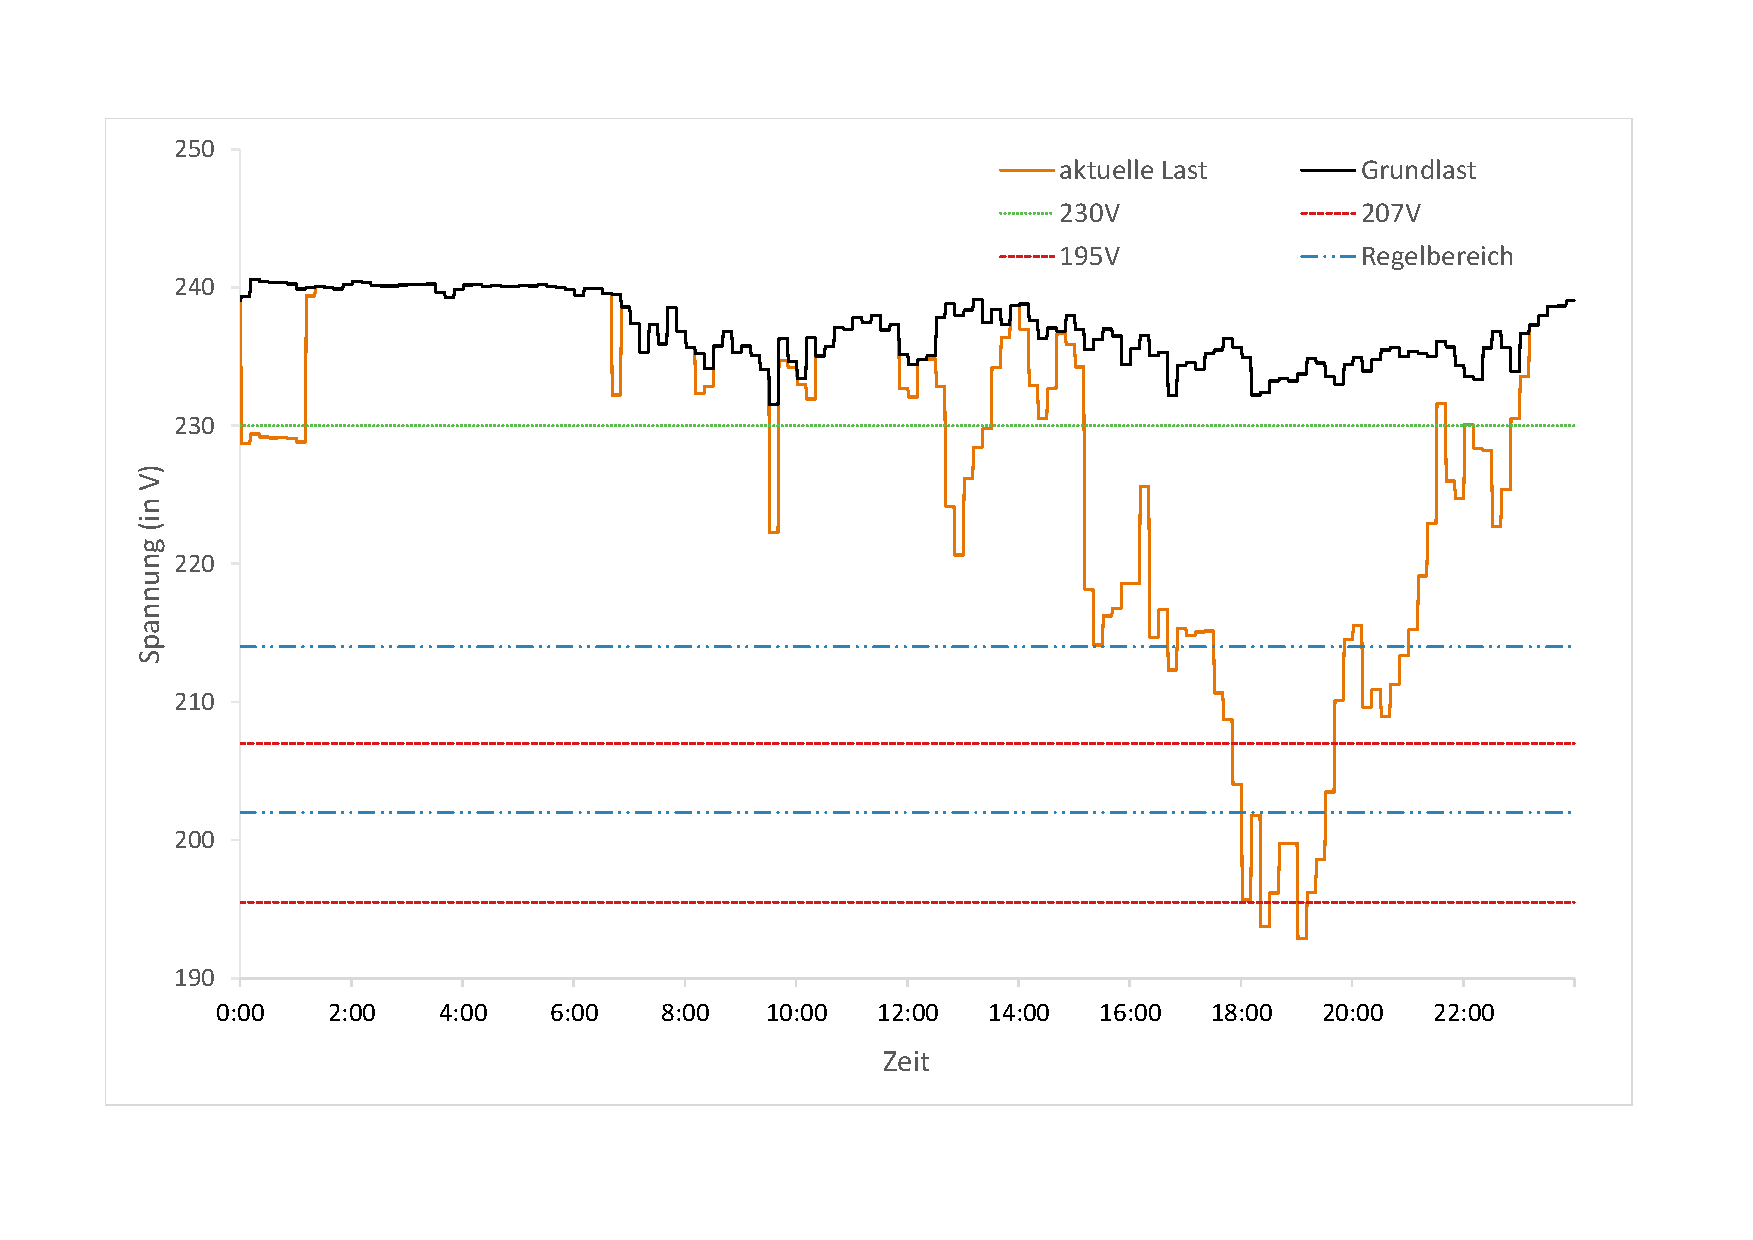
\includegraphics[scale=0.45]{img/VDE_tau/Voltage3.pdf}
	\caption{Spannungsverlauf mit 10 Minuten Mittelwerten über den Verlauf eines Tages}
	\label{Abb_VDEtauSpannung10m}
\end{subfigure}
\caption{Transformatorlast und Spannungsverlauf bei Verwendung des VDE Spannungs-Kontrollers}
\end{figure}

In der Abbildung \ref{Abb_VDEtauTrafoLast} ist die vom Transformator ans Niederspannungsnetz abgegeben Scheinleistung in kVA über den Verlauf eines Tages abgebildet. Der Regelbereich des Kontrollers ist im Falle der Transformatorlast nicht relevant, der VDE Kontroller lediglich die Spannung berücksichtigt. Die Werte schwanken stark, wenn die Werte bis an den Regelbereich ansteigen. Die starken Schwankungen der Last über die Zeit resultieren aus der Arbeit des Spannungskontrollers, welche bei zu niedrigen Spannung den möglichen Leistungsbezug reduziert. Die fehlende Stabilisierung der Werte, trotz der Verwendung des Spannungskontrollers, ist ein erstes Indiz für eine nicht ausreichende Regelung durch den verwendeten Kontroller. \\
In der Abbildung \ref{Abb_VDEtauSpannung10m} ist der Verlauf der minimalen Spannungswerte aller Anschlusspunkte über das gesamte Niederspannungsnetz hinweg aufgezeichnet. Bei den Spannungswerten handelt es sich nicht um minutengenaue Messwerte, sondern um die Mittelwerte von 10 Minuten Intervallen. Diese Intervalle wurden gewählt, um die Einhaltung der Norm DIN EN 50160 im Hinblick auf die Spannungsqualität ermittelten zu können. Die Norm befasst sich allerdings mit der Spannung an einzelnen Anschlusspunkten, dargestellt werden allerdings Werte aus dem gesamten Niederspannungsnetz, somit lässt sich anhand des Graphen nur bestimmen, ob die Norm von allen Anschlusspunkten eingehalten wurde. Bei einem sichtbaren Verstoß gegen die Norm, lässt sich nur das Vorhandensein eines einzelnen Verstoßes ableiten, da nur minimal Werte dargestellt werden. Ob zeitgleich noch andere Anschlusspunkte gegen die Norm verstoßen haben ist anhand des Graphen nicht feststellbar. Der Verlauf des Graphen zeigt, dass wenn die Werte bis zum Regelbereich abfallen, die vom Spannungskontroller vorgenommenen Regelungen nicht ausreichen, um die Spannung immer auf einem ausreichendem Niveau zu halten.
\begin{figure}[htb]
	\centering
	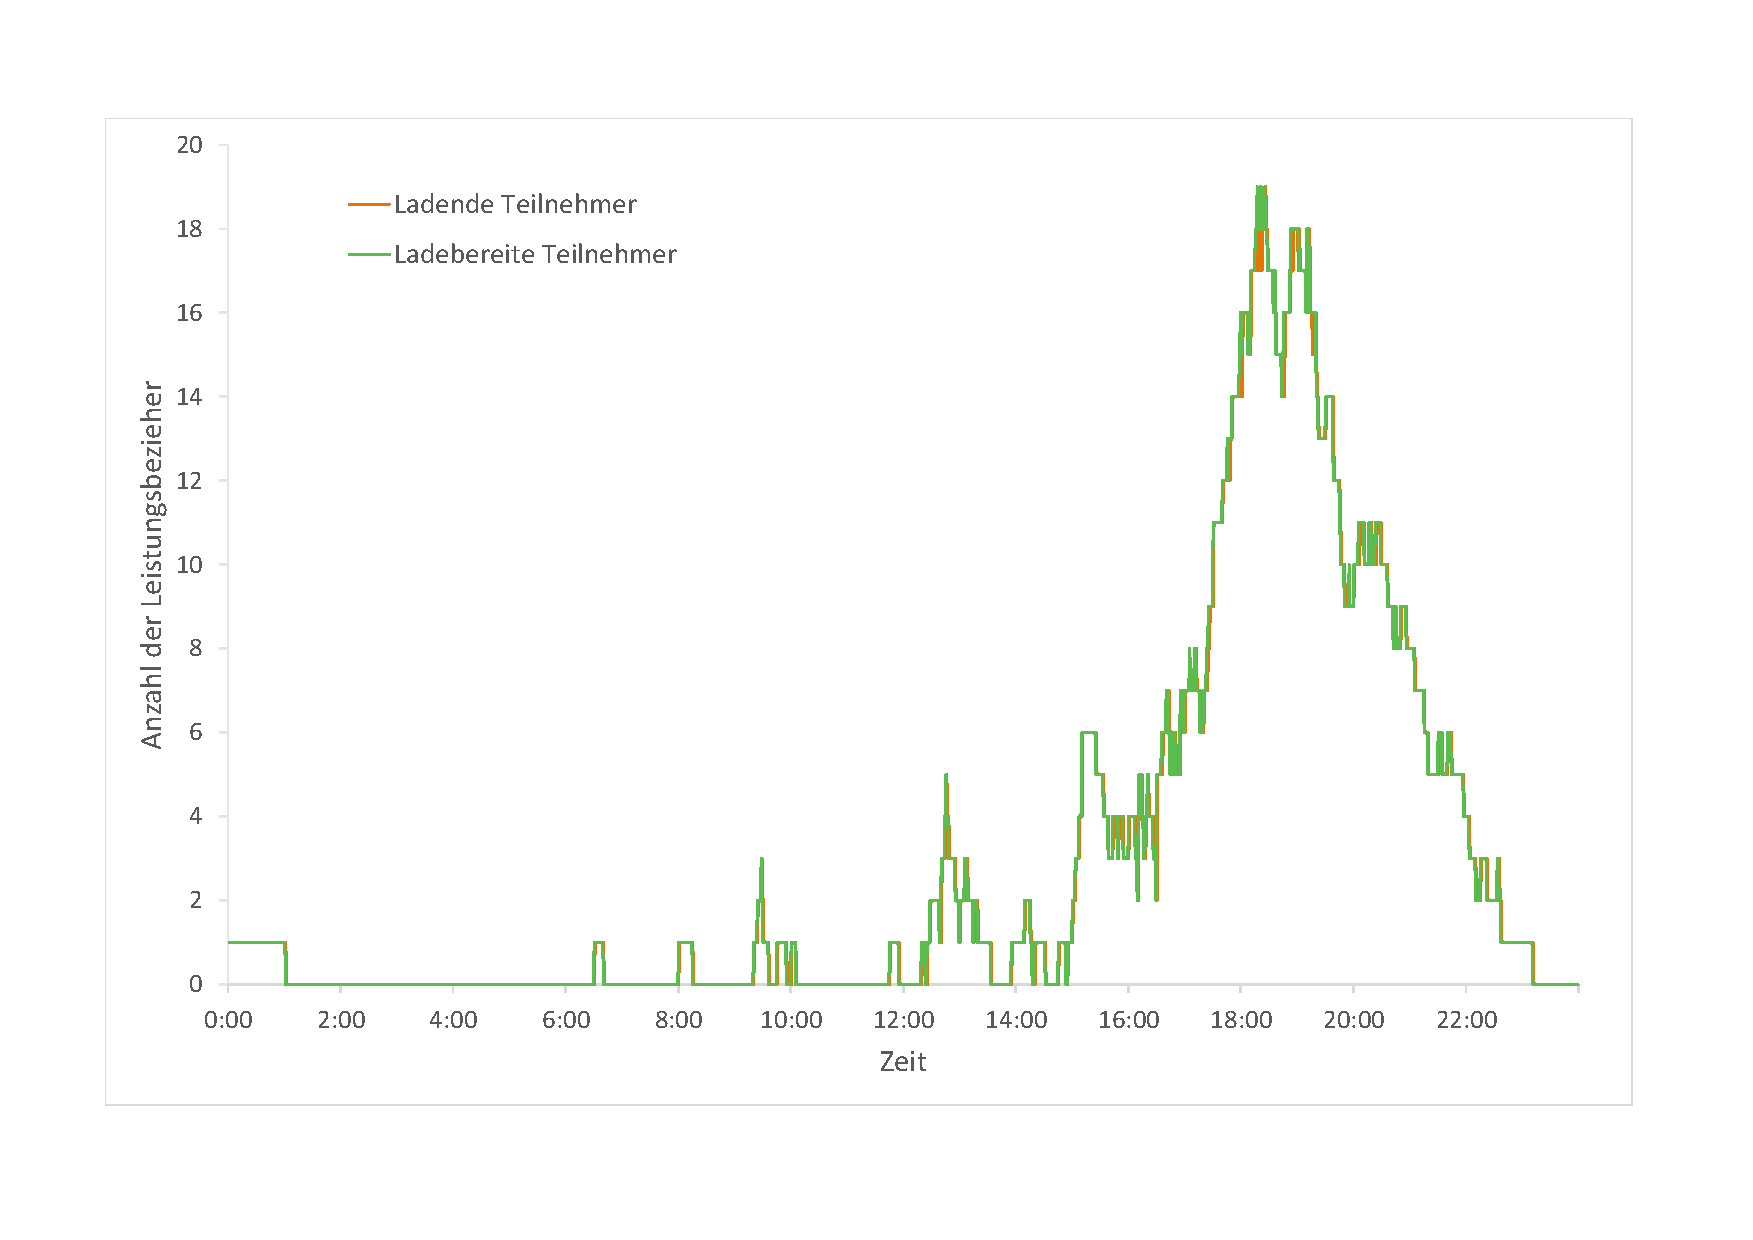
\includegraphics[scale=0.45]{img/VDE_tau/Teilnehmer3.pdf}
	\caption{Teilnehmeranzahlen bei Verwendung des VDE Spannungs-Kontrollers über den Verlauf eines Tages}
	\label{Abb_VDEtauTeilnehmer}
\end{figure}

In der Abbildung \ref{Abb_VDEtauTeilnehmer} ist die Anzahl an ladebereiten und tatsächlich ladenden Teilnehmern abgebildet. Ein Abstand zwischen den beiden Kurven weist daraufhin, dass es ladebereite Teilnehmer gibt, welche aber nicht laden. Der geringe Unterschied zwischen den beiden Kurven zeigt, dass meist alle ladebereiten Teilnehmer auch tatsächlich laden. Der Spannungskontroller ist nicht in der Lage durch den Einsatz von Wartezeiten die Anzahl an tatsächlich ladenden Teilnehmern zu verringern. Der Spannungskontroller kann eine Verringerung der Anzahl der ladenden Teilnehmer nur vornehmen, wenn sich die Spannungswerte der Teilnehmer unterhalb des Regelbereiches befinden und kein Leistungsbezug mehr erfolgen kann.\\
Im Zeitraum von 0:00 Uhr bis etwa 16:00 Uhr fällt die Spannung nicht bis in den Regelbereich ab, der verwendete Spannungskontroller muss in diesem Zeitraum nicht eingreifen. um etwa 16:00 Uhr beginnt die Anzahl an ladenden Teilnehmer zu steigen. Die steigende Anzahl an damit einhergehenden Ladevorgänge führt auch zu einem Anstieg der Transformatorlast. Durch den Anstieg der Menge an bezogener Leistung beginnt die Spannung bis in den Regelbereich abzusinken. Die Spannung sinkt bis unter den Regelbereich ab und bleibt auf diesem Niveau bis die Anzahl an Teilnehmern zurückgeht und damit auch die Transformatorlast wieder sinkt. Der Spannungskontroller an sich war nicht in der Lage die Spannung auf einem ausreichendem hohem Niveau zu halten, erst bei einem Rückgang der Teilnehmer war dies wieder möglich.\\
Die Norm der Spannungsqualität im Niederspannungsnetz wurde nicht erfüllt. Die maximale Anzahl an Unterschreitungen der Normspannung betrug zwar lediglich 21, wobei im betrachteten Zeitraum von einer Woche mit 1008 Messwerten etwa 50 Unterschreitungen zulässig wären. Es wurden allerdings zwei Unterschreitungen der Normspannung um mehr als die erlaubten 15~\%  festgestellt, daher wurde die Norm nicht erfüllt. \\
Die hier vorgestellte Methodik reagiert auf keine Art von Kollision, dennoch wurde die Anzahl von Situationen erfasst, in denen Kollisionen aufgetreten wären. Hierbei gibt es zu beachten, dass der Simulationszeitraum 10080 Schritte umfasst, welche von jedem der 110 betrachteten Fahrzeuge durchlaufen werden. Dies bedeutet es werden 1108'800 Situationen betrachtet. In 0,13~\% davon ist eine Spannungskollision aufgetreten und in 0,15~\% davon ist eine Transformatorkollision aufgetreten. In insgesamt 0,15~\% der Fälle, also 5615 Situationen, trat eine Art von Kollisionen auf. Diese Arten der Kollisionen beinhalten eine reine Spannungskollision, eine reine Transformatorkollision, sowie eine Spannungskollision und Transformatorkollision, welche zeitgleich auftreten. \\
Innerhalb des Simulation Zeitraumes werden insgesamt 557 Ladeservices gestartet, von denen alle erfolgreich abgeschlossen wurden. Dies bedeutet, dass ein jedes Fahrzeug beim Verlassen der Ladestation einen Ladezustand von 100~\% aufwies. Da alle begonnen Ladeservices erfolgreich beendet wurden, ist die Qualität der Ladeservices maximal.
\begin{figure}[h]
	\begin{subfigure}{0.49\linewidth}
		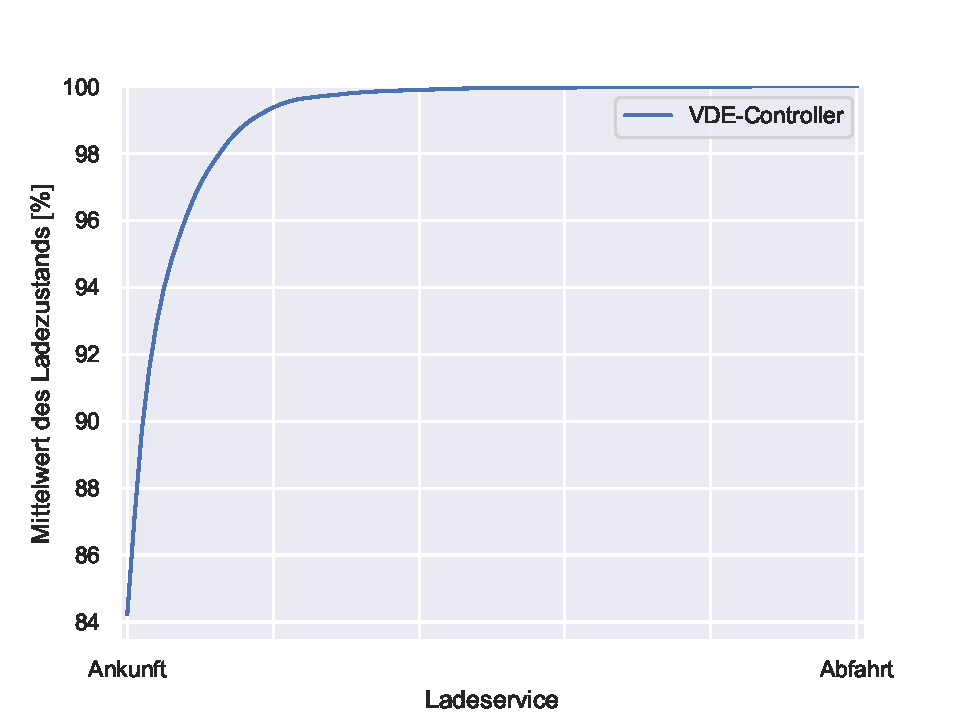
\includegraphics[width=\linewidth]{img/VDE_tau/tau_VDE_2_soc_mean.pdf}
        \subcaption{Durchschnittlicher Ladezustand \newline eines Elektrofahrzeuges über den \newline Verlauf eines Ladeservices}
        \label{ABB_VDEtauSocMEAN}
	\end{subfigure}
	\begin{subfigure}{0.49\linewidth}
		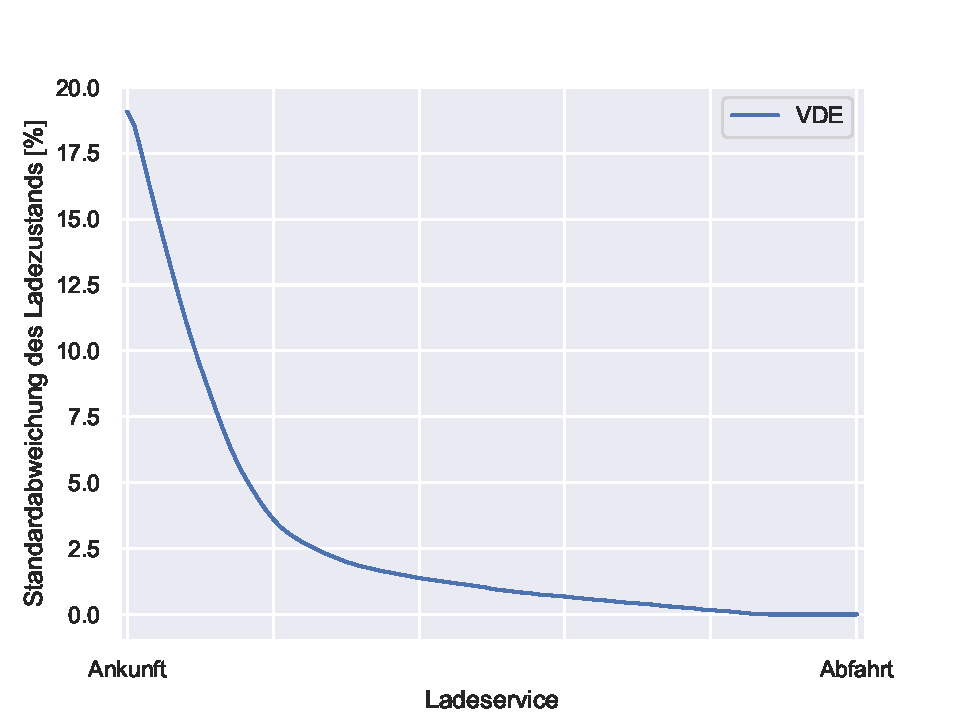
\includegraphics[width=\linewidth]{img/VDE_tau/tau_VDE_2_soc_std.pdf}
        \subcaption{Durschschnittliche Standardabweichung des Ladezustandes über den Verlauf eines Ladeservices}
        \label{ABB_VDEtauSocSTD}
	\end{subfigure}
	\caption{Durchschnittlicher Ladezustand mit Standardabweichung bei Verwendung des VDE Spannungs-Kontrollers}
\end{figure}
In Abbildung \ref{ABB_VDEtauSocMEAN} wird der mittlere Ladestand über alle Fahrzeuge im Verlauf des jeweiligen Ladeservices dargestellt. Abbildung \ref{ABB_VDEtauSocSTD} zeigt die zugehörige Standardabweichung. Der schnelle Anstieg des Ladestandes, in nur etwa 20~\% der verfügbaren Zeit liegt der Mittelwert bereits bei etwa 99 \% zeigt das viele Fahrzeuge bereits zu Beginn ihres Ladeservices einen hohen Ladezustand erreichen. Auch an der Abnahme der Standardabweichung lässt sich eine Annäherung der Werte aneinander erkennen. Die Tatsache, dass die Standardabweichung im Durchschnitt aber dennoch etwa 80~\% der Zeit benötigt um auf 0~\% zu sinken, zeigt es denoch Teilnehmer gibt, welche mehr von ihrem Ladeservice benötigen um einen Ladezustand von 100~\% zu erreichen. Dies kann an einem zeitlich kurzen Ladeservice oder an einem niedrigen Ladezustand zu Beginn des Ladeservices liegen , beide Gründe führen dazu das ein Teilnehmer mehr seines Ladeservices fürs Laden verwenden muss. Die Fairness der Ladeservice beim Erreichen dieser Qualität ist in Abbildung \ref{Abb_VDEtauFairness} aufgezeichnet. 
\begin{figure}[h]
\centering
	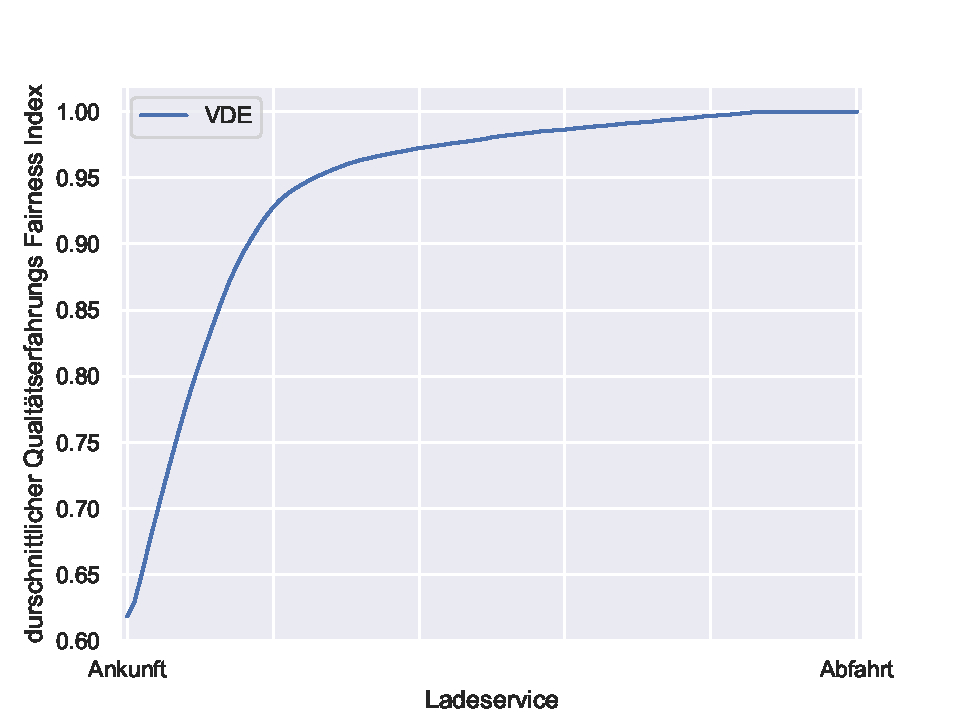
\includegraphics[scale=0.45]{img/VDE_tau/tau_VDE_2_qoe.pdf}
	\caption{Durchschnittlicher Qualitätserfahrung Fairness Index der Teilnehmer über den Verlauf des Ladeservices bei Verwendung der Methodik VDE}
	\label{Abb_VDEtauFairness}
\end{figure}

Abbildung \ref{Abb_VDEtauFairness} zeigt der durchschnittliche Qualitätserfahrungs Fairness Index aller Teilnehmer über den Verlauf der jeweiligen Ladeservice. Der Fairnessindex hängt von der Standardabweichung des Ladezustandes ab, deshalb steigt der Index wie die Standardabweichung fällt. Da, je geringer die Standardabweichung ist, desto höher ist der Fairnessindex. Da viele Fahrzeuge bereits in den Anfangszeiten ihrer Ladeservice nahe an den vollen Ladezustand herankommen, steigt auch die Fairness schnell an. Es zeigt sich aber ein ähnliches Bild, wie bei der Standardabweichung, nach einem anfänglich starken Anstieg flacht dieser Anstieg ab und es dauert bis die Fairness ihren maximal möglichen wert erreicht. Auch dies deutet darauf hin das es Teilnehmer gibt, welche mehr von ihrem Ladeservice benötigen um 100~\% Ladezustand zu erreichen.

\subsection{Slotted Aloha mit Teilnehmerzahl}
\label{chap_SApar}
Als nächsten wird auf die Ergebnisse der Simulationen eingegangen, wenn der VDE Kontroller mit Teilen des Slotted Aloha Protokolls erweitert wird. Die der Berechnung der Wartezeiten verwendet diese Methodik nur die aktuelle Anzahl an ladebereiten Teilnehmern.\\
\begin{figure}
	\begin{subfigure}{\linewidth}
		\includegraphics[scale=0.45]{img/SA_par/TrafoLast3.pdf}
		\caption{Transformatorlast über den Verlauf eines Tages}
		\label{Abb_SAparTrafoLast}
	\end{subfigure}
	\begin{subfigure}{\linewidth}
		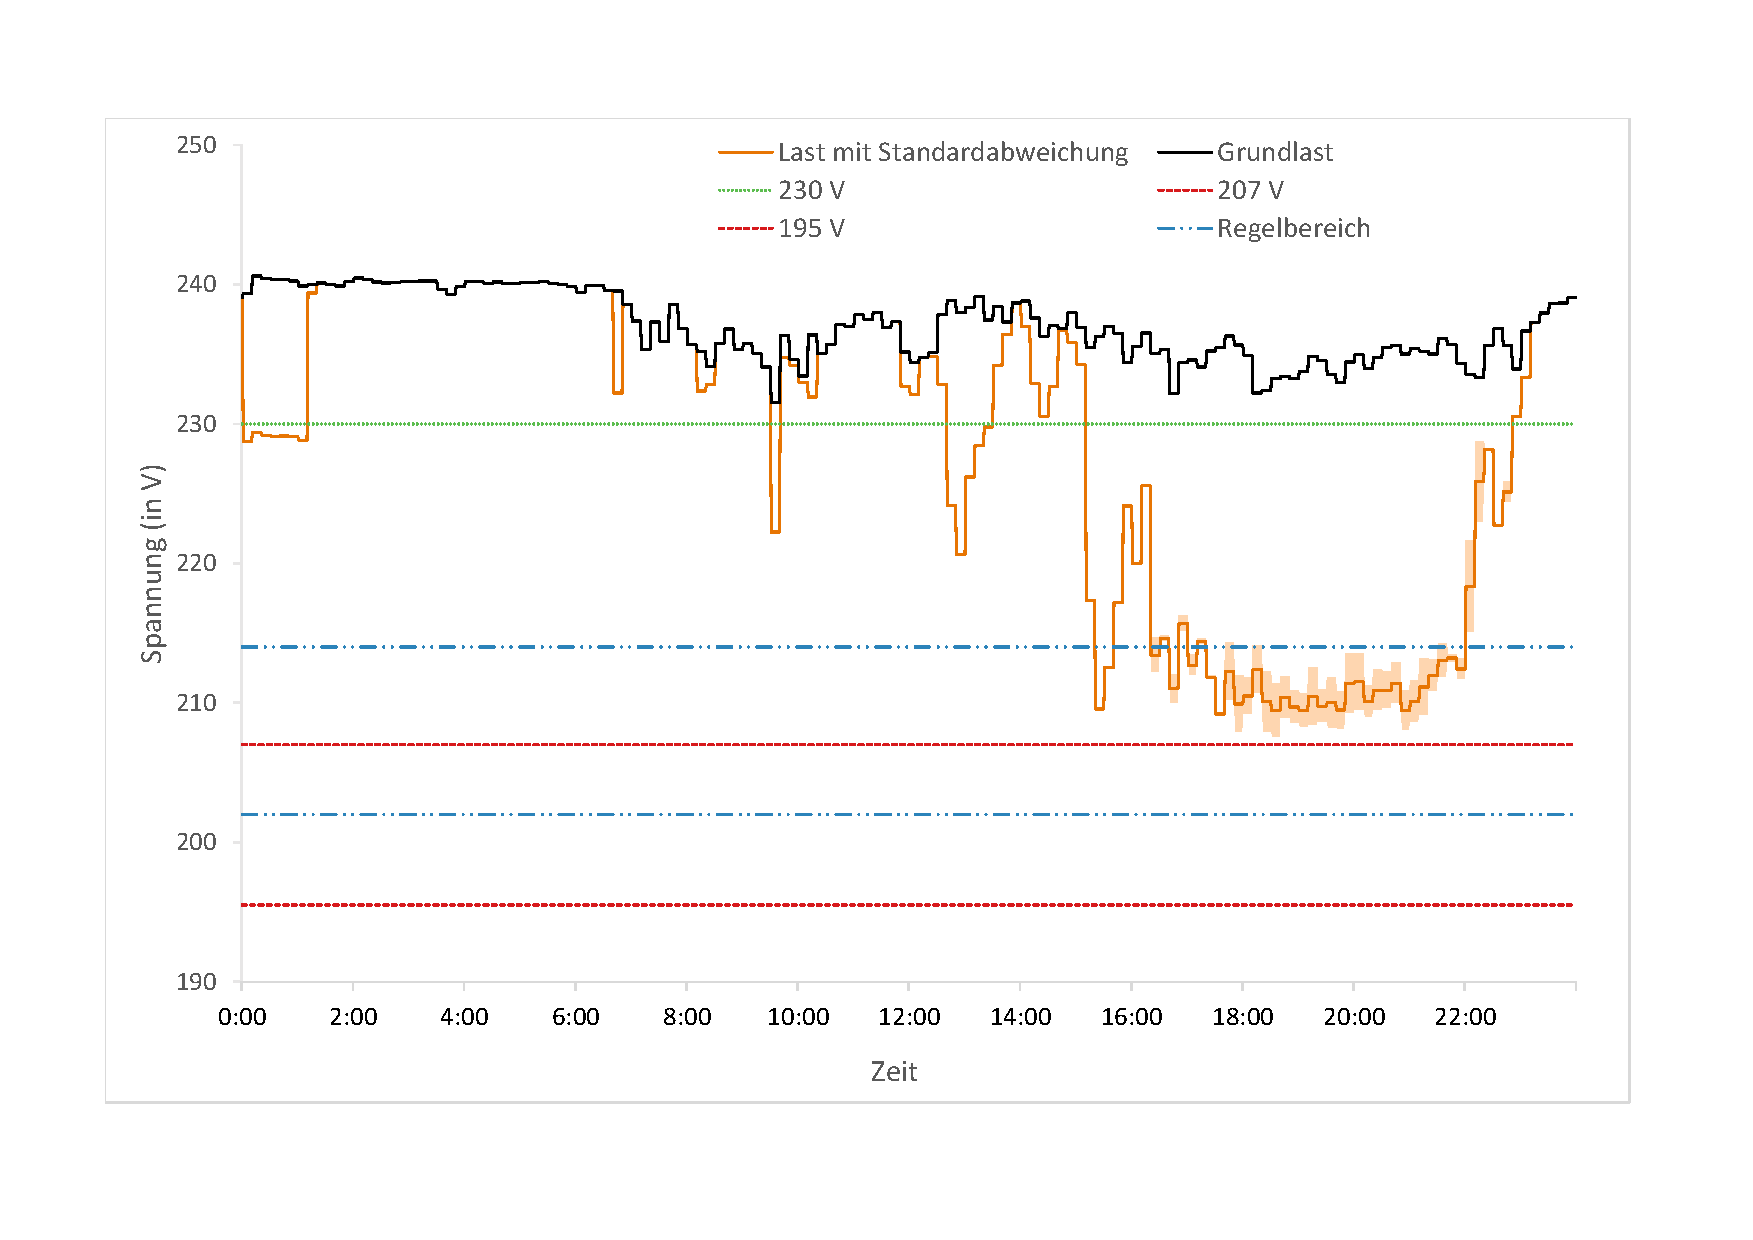
\includegraphics[scale=0.45]{img/SA_par/Voltage4.pdf}
		\caption{Spannungsverlauf mit 10 Minuten Mittelwerten über den Verlauf eines Tages}
		\label{Abb_SAparSpannung}
	\end{subfigure}
	\caption{Transformatorlast und Spannungsverlauf bei Verwendung von SA+T}
\end{figure}

In der Abbildung \ref{Abb_SAparTrafoLast} ist der Mittelwert der vom Transformator ans Niederspannungsnetz abgegebenen Scheinleistung in kVA über den Verlauf eines Tages abgebildet. Der Regelbereich des Kontrollers ist im Falle der Transformatorlast nicht relevant, da mit dieser Methodik der Transformatorkontroller nicht verwendet wird. Die hohe Standardabweichung weist auf hohe Unterschiede zwischen den einzelnen Durchläufen hin. Die Werte schwanken weniger stark und erreichen auch nicht solche Werte, wie wenn nur der VDE-Kontroller verwendet wird. Daraus lässt sich ableiten, das schon die Erweiterung mit dem Slotted Aloha Protokoll dazu beiträgt die Transformatorlast zu kontrollieren, da durch Verwendung von Wartezeiten ladebereite Teilnehmer nicht laden und so auch keine Leistung beziehen. \\
Abbildung \ref{Abb_SAparSpannung} zeigt den Verlauf der minimalen Spannungswerte samt Standardabweichung aller Teilnehmer des Niederspannungsnetz hinweg, als Werte dienen auch hier die Mittelwerte von 10-minütigen Intervallen. In diesem Fall zeigt die Standardabweichung keine solche Unterschiede zwischen den Durchläufen, wie bei der Transformatorlast. Wenn die Werte bis in den Regelbereich hinein abfallen, bleiben sie innerhalb des Regelbereiches stabil und fallen auch nicht unter den Regelbereich ab. Wie bei der Transformatorlast zeigt sich auch hier der Einfluss der Wartezeiten, durch diesen verbleiben die Werte zwar eine längere Zeitspanne im Regelbereich, die Werte fallen aber nicht so weit ab wie ohne Wartezeiten.
\begin{figure}[htb]
\centering
	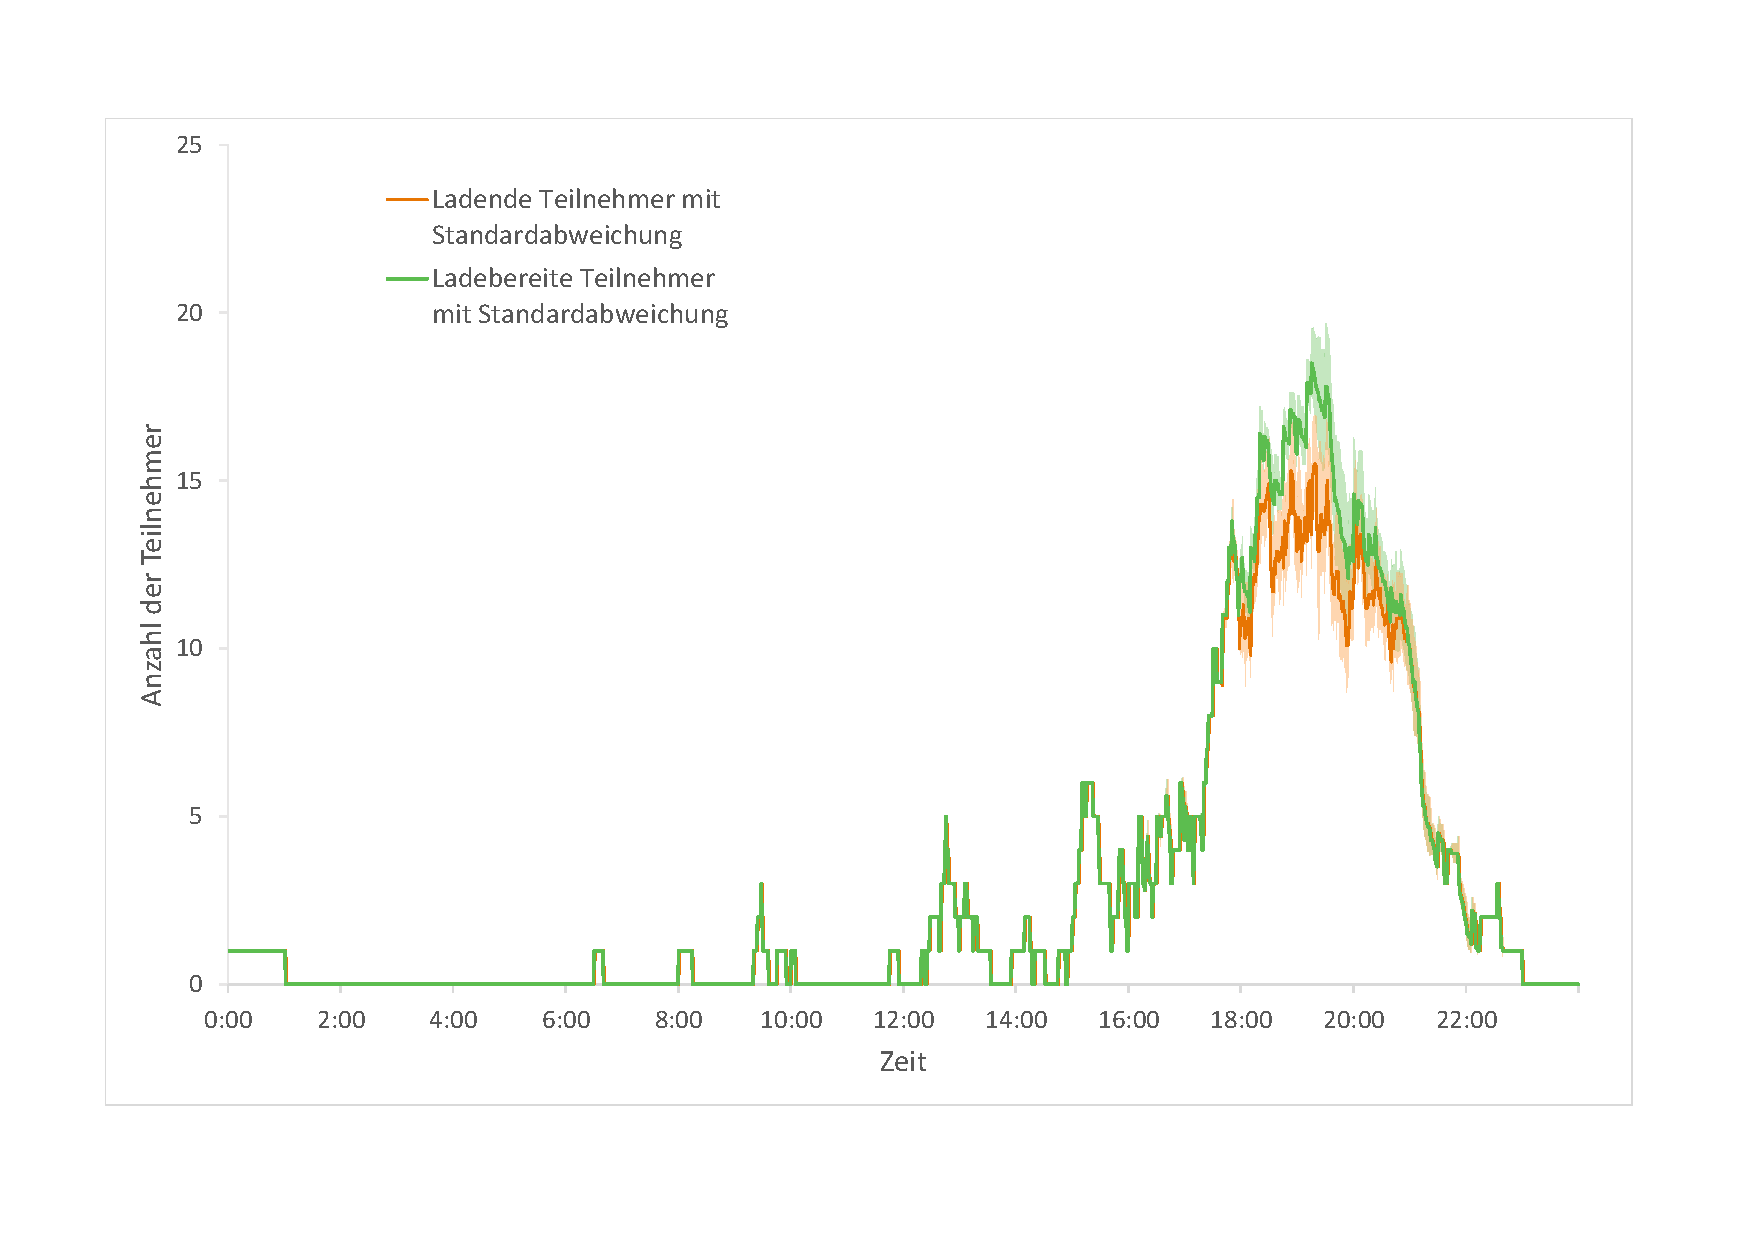
\includegraphics[scale=0.45]{img/SA_par/Teilnehmer2.pdf}
	\caption{Teilnehmerzahlen bei Verwendung von SA+T über den Verlauf eines Tages}
	\label{Abb_SAparTeilnehmer}
\end{figure}
In Abbildung \ref{Abb_SAparTeilnehmer} ist die Anzahl an ladebereiten und ladenden Teilnehmern mit der jeweiligen Standardabweichung dargestellt. Die auch hier teils hohe Standardabweichung weist wieder auf größerer Unterschiede zwischen den Durchläufen hin. Die hier vorgestellte Methodik arbeitet mit Wartezeiten und ist durch diese in der Lage die Anzahl an ladenden Teilnehmern zu verringern. Die Anstiege der ladenden Teilnehmer ohne einen dazugehörigen Anstieg der ladebereiten Teilnehmer weist darauf hin, das bei mehreren Teilnehmern gleichzeitig die Wartezeit abgelaufen ist und diese Teilnehmer gehäuft wieder zu laden beginnen. Diese Stellen zeigen, die Teilnehmer werden zwar zeitlich verteilt, allerdings begünstigt die geringe Menge an Auswahlmöglichkeiten, in diesem Fall die Anzahl ladebereiter Teilnehmer, das Auftreten solcher Häufungen. \\
Bis etwa 16:00 Uhr steigt sowohl die Grundlast und somit auch die Transformatorlast als ganzes zwar mehrmals an, jedoch fällt die Spannung dadurch nie bis zum Regelbereich hin ab. Um etwa 16:00 Uhr fällt die Spannung erstmals in den Regelbereich ab, steigt dann allerdings wieder an. Dieser Spannungsfall lässt sich auf einen erhöhten Leistungsbedarf von der steigenden Anzahl an Teilnehmern zurückführen. Da die Anzahl an Teilnehmer nur kurz ansteigt, steigt auch die Spannung wieder an. Nach 16:00 Uhr fällt der Minimalwert der Spannung für etwa 6 Stunden bis in den Regelbereich ab. Im selben Zeitraum kommt es auch zu einem erhöhten Leistungsabgabe am Transformator, und auch die Anzahl der Teilnehmer steigt an auf bis zu 18 Teilnehmer. Innerhalb der Zeitspanne in der sich die Spannungswerte im Regelbereich des Spannungskontrollers befinden schwanken die minimalen Werte nur gering. Diese geringe Schwankung lässt den Schluss zu das diese Variante des Kontrollers in der Lage ist die Spannung im Niederspannungsnetz effektiv zu regeln und auf einem ausreichenden Niveau zu halten. \\
Im gesamten betrachteten Zeitraum von einer Woche kommt es zu keiner Unterschreitung von mehr als 15~\% der Normspannung sowie zu lediglich im Durchschnitt etwa 0,4 Unterschreitungen um mehr als 10~\% der Normspannung. Die Norm DIN EN 50160 wird folglich erfüllt, da die betrachteten Grenzwerte innerhalb der erlaubten Bereiche liegen.\\
Über den Simulationszeitraum hinweg wurden im Schnitt 668,7 Situationen ($\pm$ 6,7~\%) festgestellt, in denen Spannungswerte gemessen wurden, welche eine Spannungskollision verursachen könnten. In 553,9 dieser 668,7 Situationen ($\pm$ 5,9~\%) trat tatsächlich eine Spannungskollision auf und eine Wartezeit wurde berechnet. Der Simulationszeitraum umfasst 10080 Zeitschritte für 110 Teilnehmer, folglich wurden 1108800 Situationen betrachtet. Die 553,9 Situationen stellen also 0,04~\% der insgesamt betrachteten Situationen dar. Die hier verwendete Methodik reagiert nur auf Spannungskollisionen, die Menge von Situationen in denen eine Transformatorkollision auftreten könnte wurde dennoch erfasst. In durchschnittlich 7514,5 ($\pm$ 2,0 \%) der betrachteten Situationen wurde ein Verstoß gegen den Grenzwert der Transformatorlast festgestellt, was etwa 0,67~\% aller Situation entspricht.\\
\begin{figure}
	\begin{subfigure}{0.49\linewidth}
		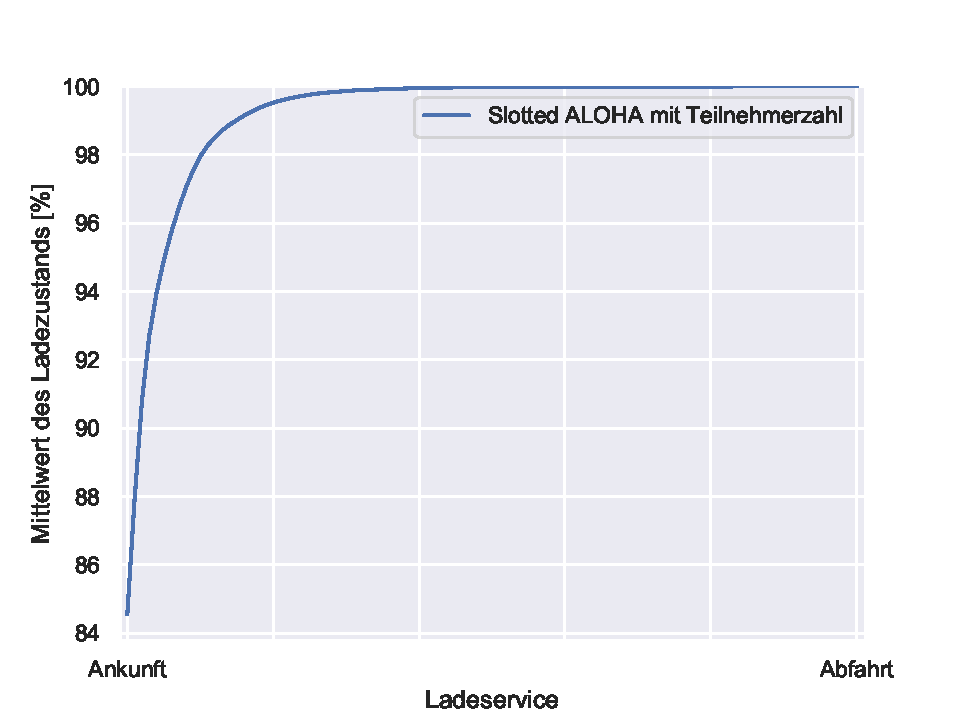
\includegraphics[width=\linewidth]{img/SA_par/SlottedAloha_participants_VDE_tau_10_soc_mean.pdf}
        \subcaption{Durchschnittlicher Ladezustand eines Elektrofahrzeuges über den Verlauf eines Ladeservices}
        \label{ABB_SAparSocMEAN}
	\end{subfigure}
	\begin{subfigure}{0.49\linewidth}
		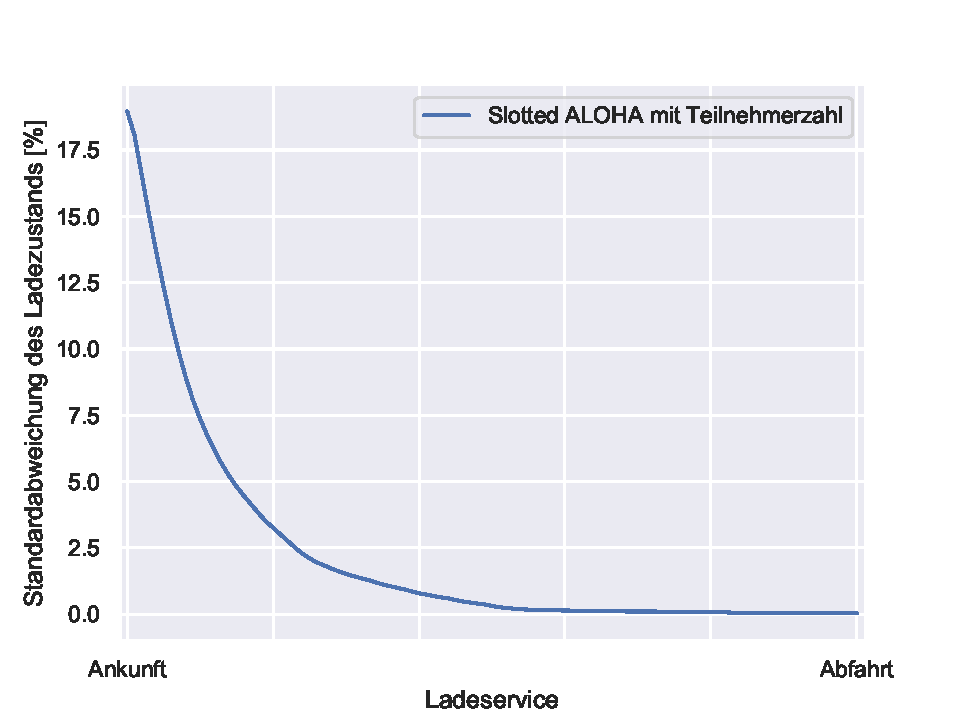
\includegraphics[width=\linewidth]{img/SA_par/SlottedAloha_participants_VDE_tau_10_soc_std.pdf}
        \subcaption{Durschschnittliche Standardabweichung des Ladezustandes über den Verlauf eines Ladeservices}
        \label{ABB_SAparSocSTD}
	\end{subfigure}
	\caption{Durchschnittlicher Ladezustand mit Standardabweichung bei Verwendung der Methodik SA+T}
\end{figure}
Alle 557 gestarteten Ladeservices wurden erfolgreich abgeschlossen, somit ist die Qualitätserfahrung aller Ladevorgänge maximal. Abbildung \ref{ABB_SAparSocMEAN} zeigt den durchschnittlichen Ladezustand über den Verlauf eines Ladeservices hinweg, Abbildung \ref{ABB_SAparSocSTD} zeigt die zugehörige Standardabweichung. Der schnelle Anstieg des mittleren Ladestandes zu Beginn zeigt auch hier das viele der Teilnehmer bereits zu Beginn ihres Ladeservices einen hohen Ladestand nahe des Ziels von 100~\% erreichen. Der Verlauf der Standardabweichung zeigt allerdings auch hier, das trotz einer schnellen Abnahme zu Beginn, dennoch etwa 80~\% eines Ladeservicesaufgewendet werden müssen, bis die Standardabweichung auf 
0~\% zurückgegangen ist. Dies weist auf die Unterschiede zwischen den Ladestanden zu Beginn der Ladeservice hin, wobei manche Teilnehmer mit niedrigeren ladezuständen auch mehr Zeit benötigen um einen ladestand von 100~\% zu erreichen.
\begin{figure}[htb]
\centering
	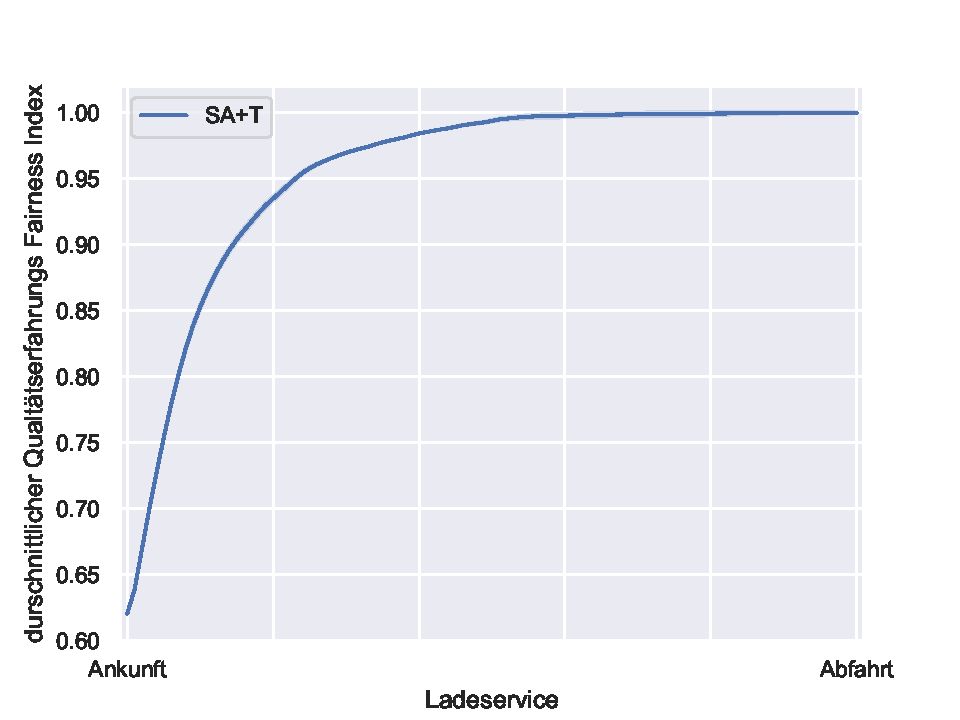
\includegraphics[scale=0.45]{img/SA_par/SlottedAloha_participants_VDE_tau_10_qoe.pdf}
	\caption{Durchschnittlicher Qualitätserfahrung Fairness Index der Teilnehmer über den Verlauf des Ladeservices bei Verwendung der Methodik SA+T}
	\label{Abb_SAparFairness}
\end{figure}
Abbildung \ref{Abb_SAparFairness} zeigt den Fairness Index der jeweiligen Qualitätserfahrung mit der dazugehörigen Standardabweichung über den Zeitverlauf der Ladeservices. Die Qualität des Ladeservices hängt von der Standardabweichung des Ladezustandes ab. Die Standardabweichung des Graphen ist sehr gering, dies deutet auf sehr ähnliche Ergebnisse über alle absolvierten Durchläufe hin. Der Verlauf zeigt auch hier nach einem starken Anstieg zu Beginn ein Abflachen der Steigung, auch dies weist auf Teilnehmer hin welche mehr ihres Ladeservices benötigen um einen hohen Ladestand zu erreichen.

\subsection{Slotted Aloha mit Teilnehmerzahl und Fahrzeugparametern}
\label{chap_SAwt}
Hier wird auf die Ergebnisse bei der Verwendung des Spannungskontrolles, welcher mit Slotted Aloha erweitert wurde und die Teilnehmeranzahl und die Fahrzeugparameter miteinbezieht, eingegangen. 
\begin{figure}
	\begin{subfigure}{\linewidth}
		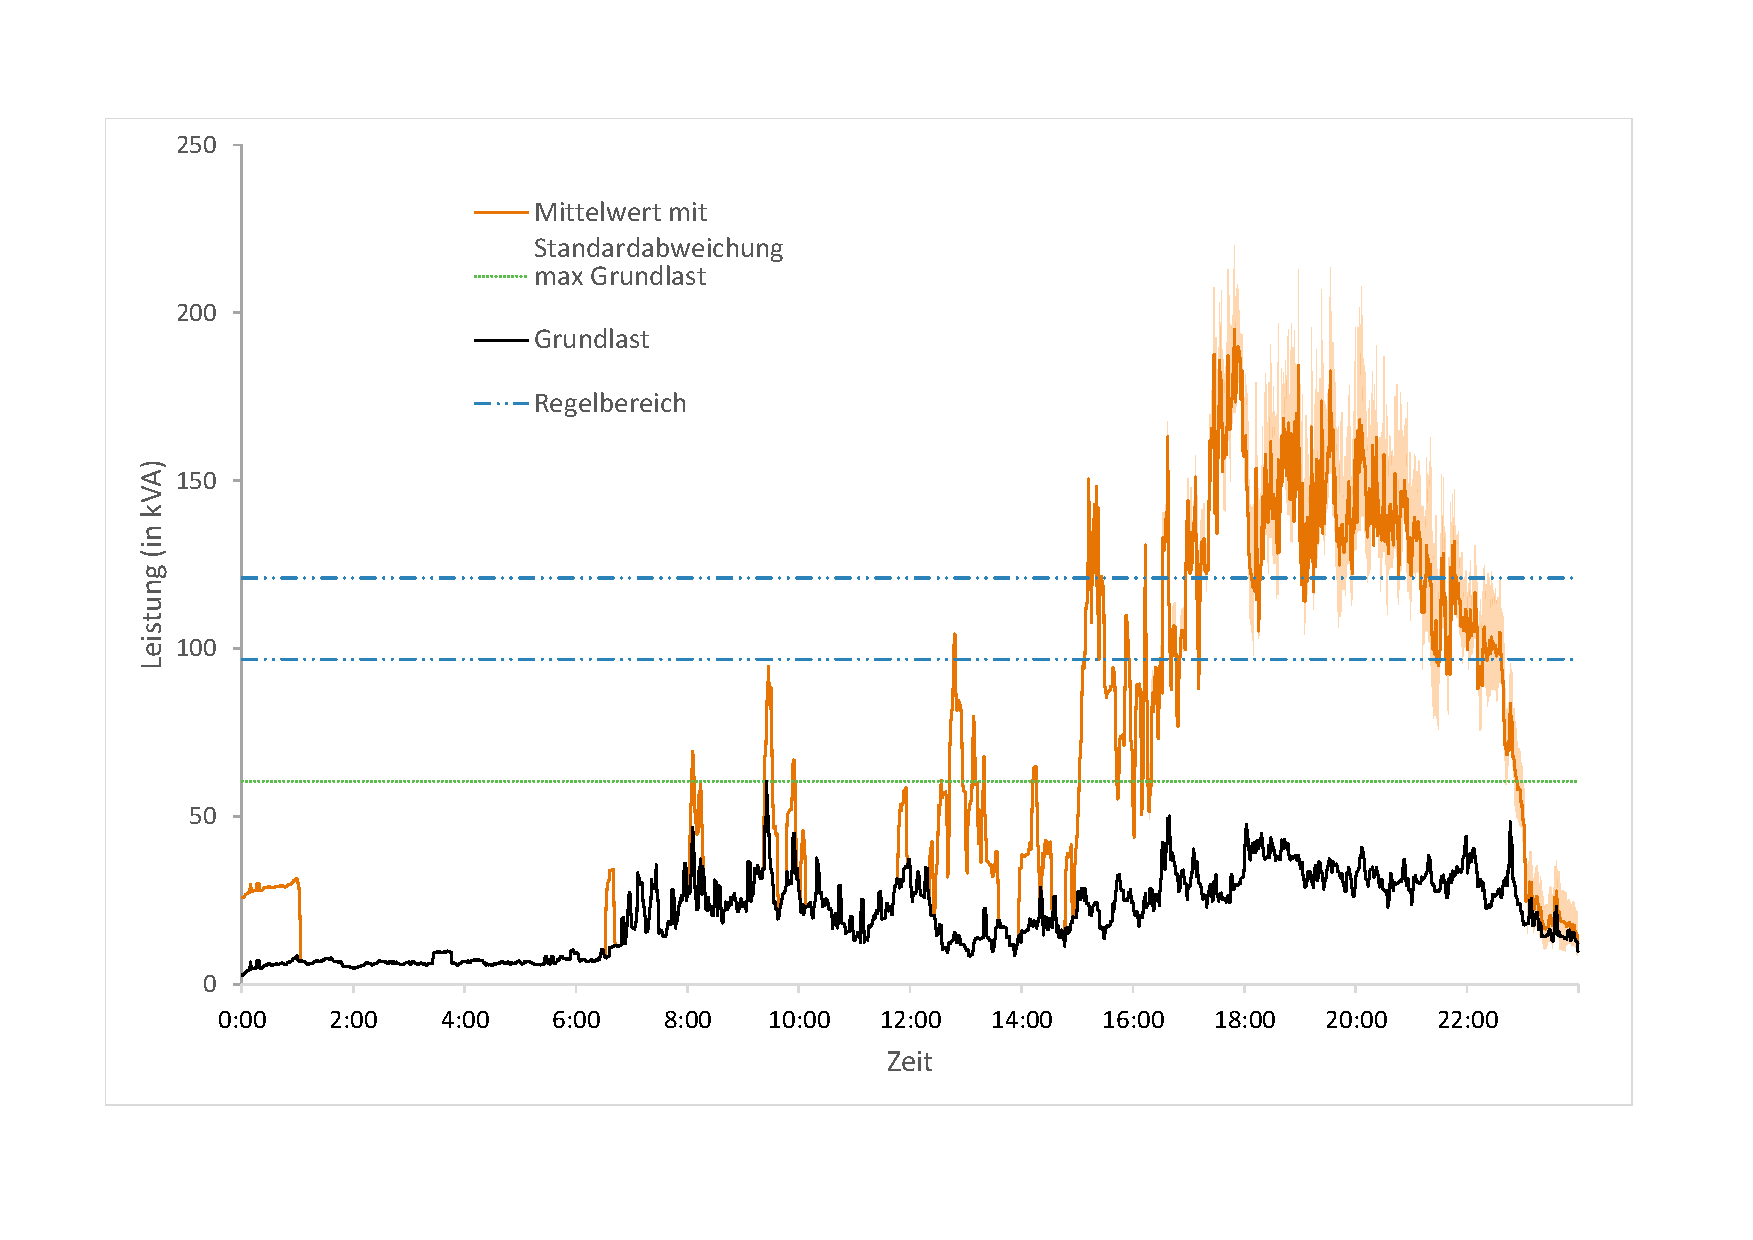
\includegraphics[scale=0.45]{img/SA_wT/TrafoLast5.pdf}
		\caption{Transformatorlast über den Verlauf eines Tages}
		\label{Abb_SAwtTrafoLast}
	\end{subfigure}
	\begin{subfigure}{\linewidth}
		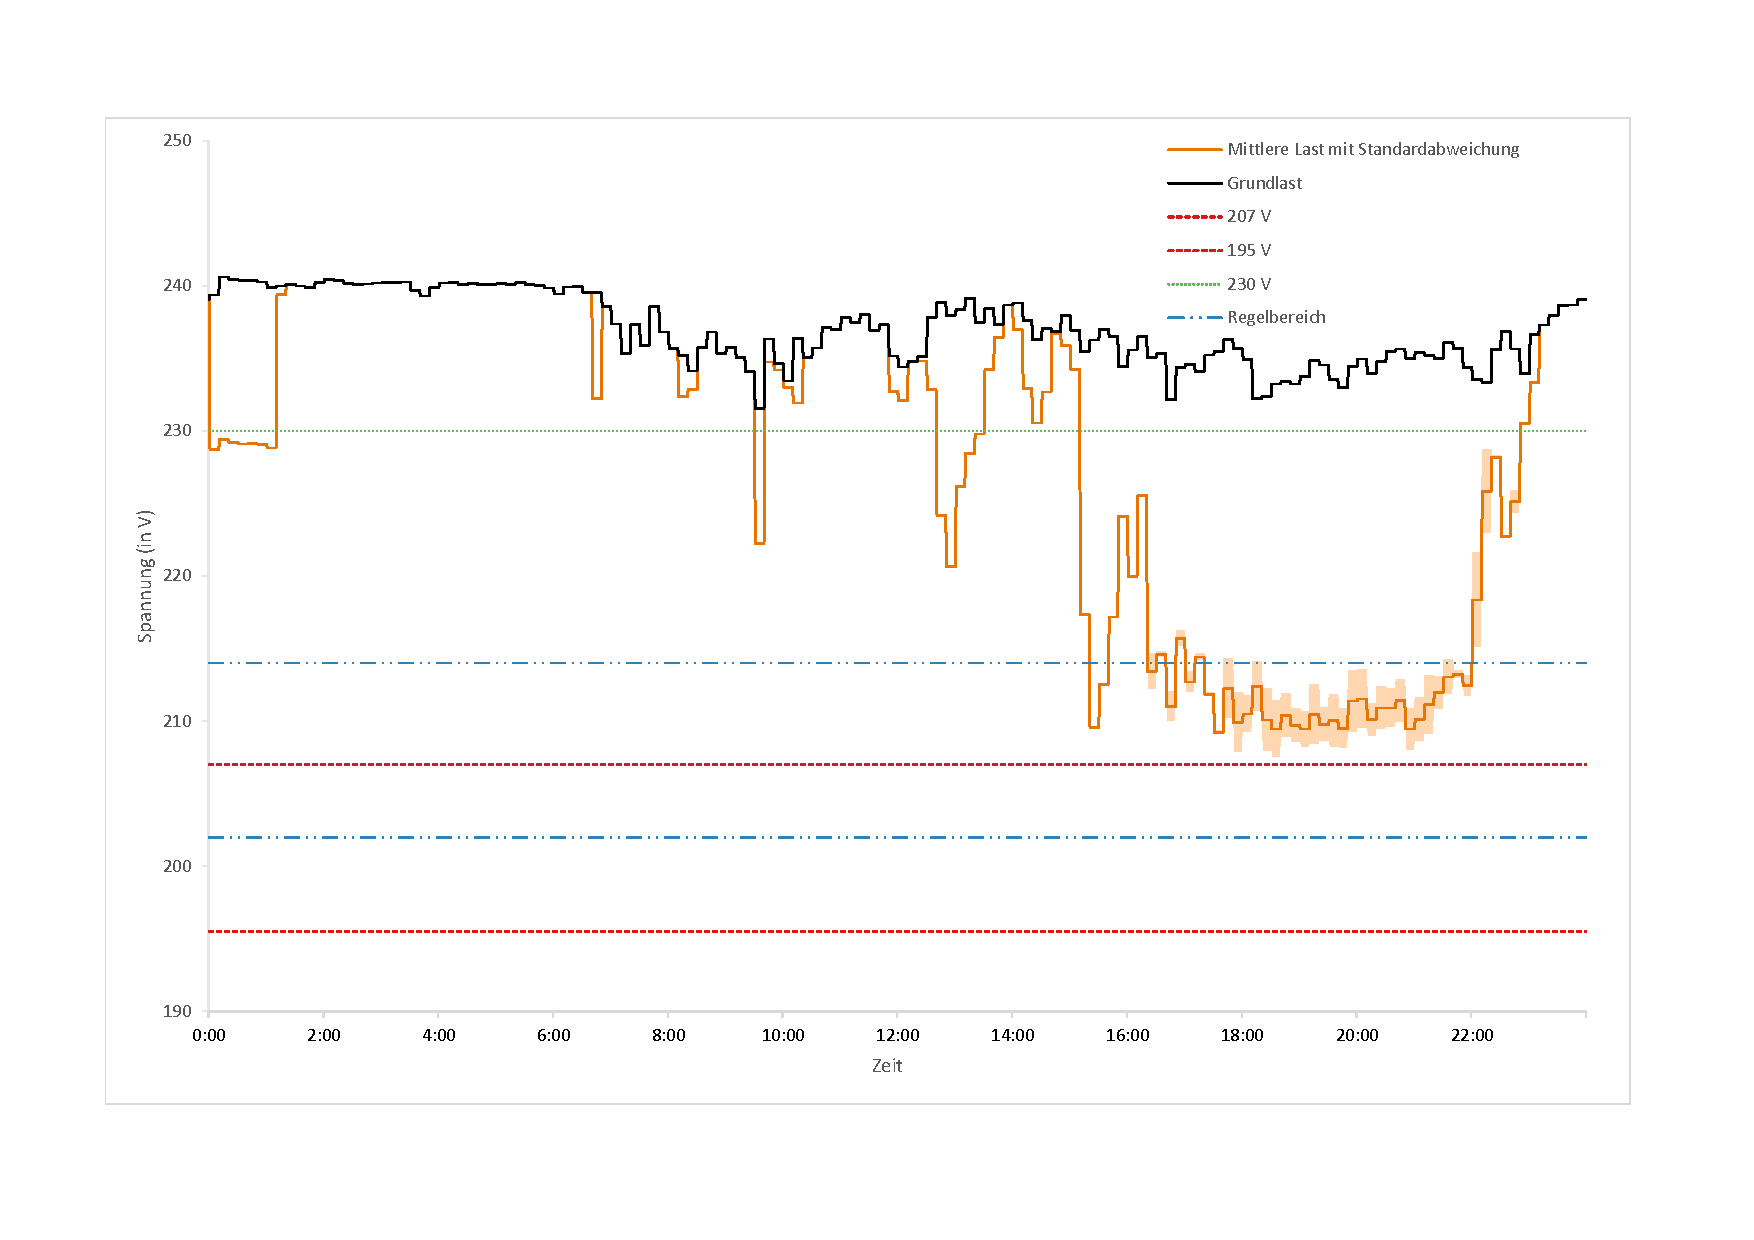
\includegraphics[scale=0.45]{img/SA_wT/Voltage2.pdf}
		\caption{Spannungsverlauf in 10 Minuten Intervallen über den Verlauf eines Tages}
		\label{Abb_SAwtSpannung}
	\end{subfigure}
	\caption{Transformatorlast und Spannungsverlauf bei Verwendung von SA+T+F}
\end{figure}

In der Abbildung \ref{Abb_SAwtTrafoLast} ist die vom Transformator ans Niederspannungsnetz abgegeben Scheinleistung in kVA über den Verlauf eines Tages abgebildet. Der Regelbereich des Kontrollers ist im Falle der Transformatorlast nicht relevant, der VDE Kontroller lediglich die Spannung berücksichtigt. Die niedrige Standardabweichung weist auf geringe Unterschiede zwischen den Durchläufen hin.Hier zeigen sich, ähnlich wie bei den Ergebnissen von SA+T, weniger Schwankungen und niedrigere Werte als bei der Verwendung des reinen VDE-Kontrollers. So zeigt sich auch hier der Einfluss der Wartezeiten, welche durch die Verteilung der Ladevorgänge auch den zugehörigen Lastbezug verteilen.\\
Abbildung \ref{Abb_SAwtSpannung} zeigt den Verlauf der minimalen Spannung über das gesamte Niederspannungsnetz hinweg mit der zugehörigen Standardabweichung. Die teils höhere Standardabweichung weist auf einige Unterschiede zwischen den einzelnen Durchläufen hin. Wie bereits bei SA+T zeigt sich auch hier das die Verteilung der Ladevorgänge durch den Einsatz von Wartezeiten zu höheren Spannungen führt, welche dann aber auch erst später wieder der Normspannung annähert.
\begin{figure}[htb]
\centering
	\includegraphics[scale=0.45]{img/SA_wT/Teilnehmer3.pdf}
	\caption{Teilnehmerzahlen bei Verwendung von SA+T+F über den Verlauf eines Tages}
	\label{Abb_SAwtTeilnehmer}
\end{figure}

In der Abbildung \ref{Abb_SAwtTeilnehmer} ist die Anzahl an ladebereiten und tatsächlich ladenden Teilnehmern samt der jeweiligen Standardabweichung abgebildet. Anders als bei der Methodik SA+T ist die Form der beiden Kurven hier ähnlicher, dies deutet daraufhin wenn sich die Anzahl an ladenden Teilnehmern erhöht, dies aufgrund einer Erhöhung der Teilnehmerzahl an sich geschieht. Ebenso zeigt es, dass die Verteilung der Teilnehmer durch das Einbeziehen der Fahrzeugparameter besser gelingt, als wenn nur die Teilnehmerzahl verwendet wird. \\
Die Aktivitäten bis etwa 16:00 Uhr führen zwar immer wieder zu einem Absinken der Spannung, jedoch erreichen die Werte dabei den Regelbereich des Kontrollers nicht. Um etwa 16:00 Uhr fällt der Spannungswert das erste Mal bis in den Regelbereich hinein ab, erholt sich dann aber wieder. Dieser kurze Abfall lässt sich auf eine kurzfristig ansteigende Anzahl an Teilnehmer und so auch steigende Transformatorlast zurückführen. Von etwa 17:00 Uhr bis 21:00 Uhr befinden sich die Mittelwerte der Minimalspannung durchgängig im Regelungsbereich des Kontrollers. Die Werte bewegen sich im Bereich von 217 V bis 210 V. Die geringe Schwankung der Werte sowie fehlende Unterschreitungen des Regelbereiches lässt den Schluss zu das diese Variante des Kontrollers dazu in der Lage ist die Spannung effektiv zu regeln und sie auf einem ausreichenden Niveau zu halten.
Im gesamten betrachteten Zeitraum von einer Woche kommt es zu keiner Unterschreitung der 195 Voltmarke sowie zu lediglich im Durchschnitt etwa 0,4 Unterschreitungen der 207 Volt Marke. Die Norm DIN EN 50160 wird folglich erfüllt, da die betrachteten Grenzwerte innerhalb der erlaubten Bereiche liegen.\\
Über den Simulationszeitraum hinweg wurden im Schnitt 392,6 Situationen ($\pm$ 12,2~\%) festgestellt, in denen Spannungswerte gemessen wurden, welche eine Spannungskollision verursachen könnten. In 246,9 dieser 392,6 Situationen ($\pm$ 9,2~\%) trat tatsächlich eine Spannungskollision auf und eine Wartezeit wurde berechnet. Der Simulationszeitraum umfasst 10080 Zeitschritte für 110 Teilnehmer, folglich wurden 1108800 Situationen betrachtet. Die 246,9 Situationen stellen also 0,02~\% der insgesamt betrachteten Situationen dar. Die hier verwendete Methodik reagiert nur auf Spannungskollisionen, die Menge von Situationen in denen eine Transformatorkollision auftreten könnte wurde dennoch erfasst. In durchschnittlich 9271,5 ($\pm$ 3,3~\%) der betrachteten Situationen wurde ein Verstoß gegen den Grenzwert der Transformatorlast festgestellt, was etwa 0,83~\% aller Situationen entspricht.\\
\begin{figure}
	\begin{subfigure}{0.49\linewidth}
		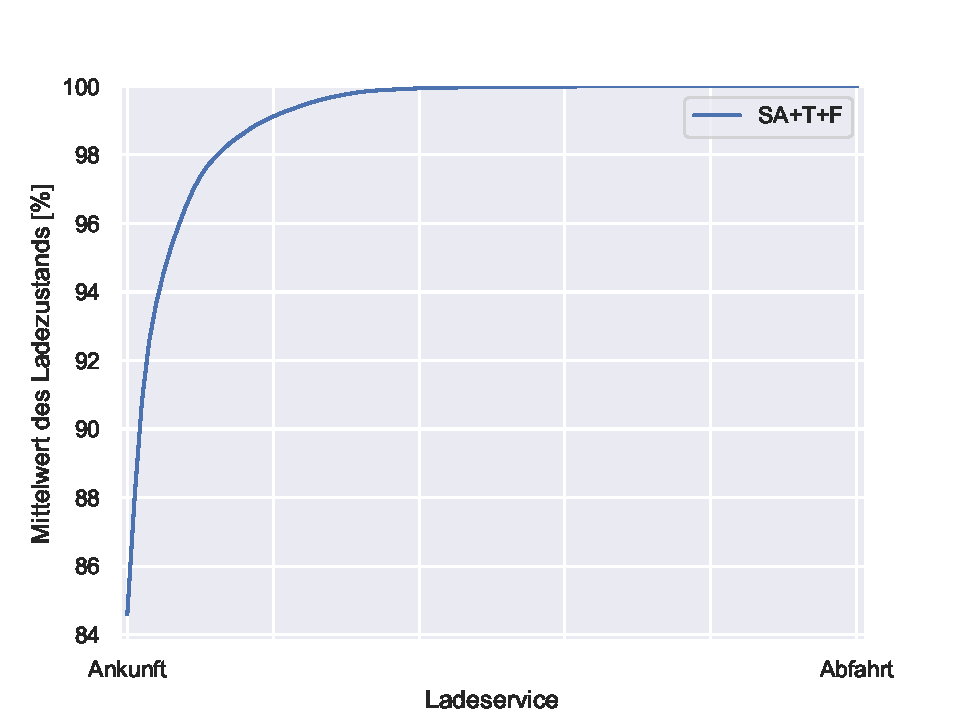
\includegraphics[width=\linewidth]{img/SA_wT/SlottedAloha_waitingTime_VDE_tau_6_soc_mean.pdf}
        \subcaption{Durchschnittlicher Ladezustand eines Elektrofahrzeuges über den Verlauf eines Ladeservices}
        \label{ABB_SAwtSocMEAN}
	\end{subfigure}
	\begin{subfigure}{0.49\linewidth}
		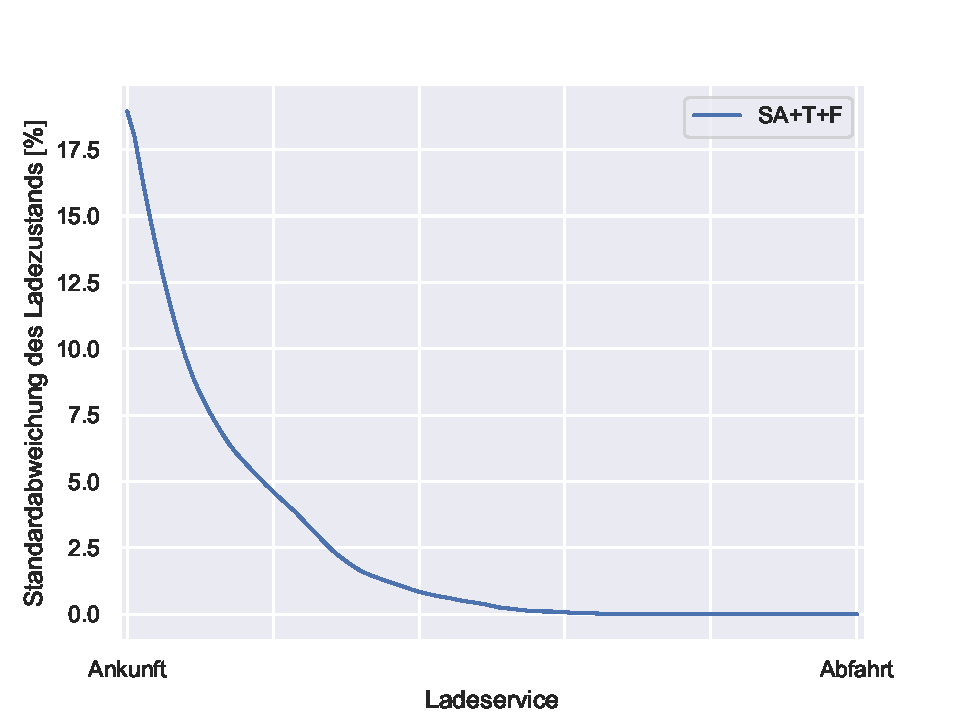
\includegraphics[width=\linewidth]{img/SA_wT/SlottedAloha_waitingTime_VDE_tau_6_soc_std.pdf}
        \subcaption{Durschschnittliche Standardabweichung des Ladezustandes über den Verlauf eines Ladeservices}
        \label{ABB_SAwtSocSTD}
	\end{subfigure}
	\caption{Durchschnittlicher Ladezustand mit Standardabweichung bei Verwendung der Methodik SA+T+F}
\end{figure}

Alle 557 gestarteten Ladeservices wurden erfolgreich abgeschlossen, somit ist die Qualitätserfahrung aller Ladevorgänge maximal. Abbildung \ref{ABB_SAwtSocMEAN} zeigt den durchschnittlichen Ladezustand über den Verlauf eines Ladeservices hinweg, Abbildung \ref{ABB_SAwtSocSTD} zeigt die zugehörige Standardabweichung. Ein schneller Anstieg des mittleren Ladezustands zeigt viele Teilnehmer bereits zu Beginn des jeweiligen Ladeservices eien hohen Ladestand erreichen. Die Standardabweichung weist aber auch hier daraufhin das es Teilnehmer gibt, welche mehr ihres Ladeservices benötigen um ihren Ladestand auf 100~\% zu erhöhen. Dieser größere Anteil liegt entweder an einem generell kürzeren Zeitraum für den Ladeservice oder einem niedrigen Ladestand beim beginn des Ladeservice.\\
\begin{figure}[htb]
\centering
	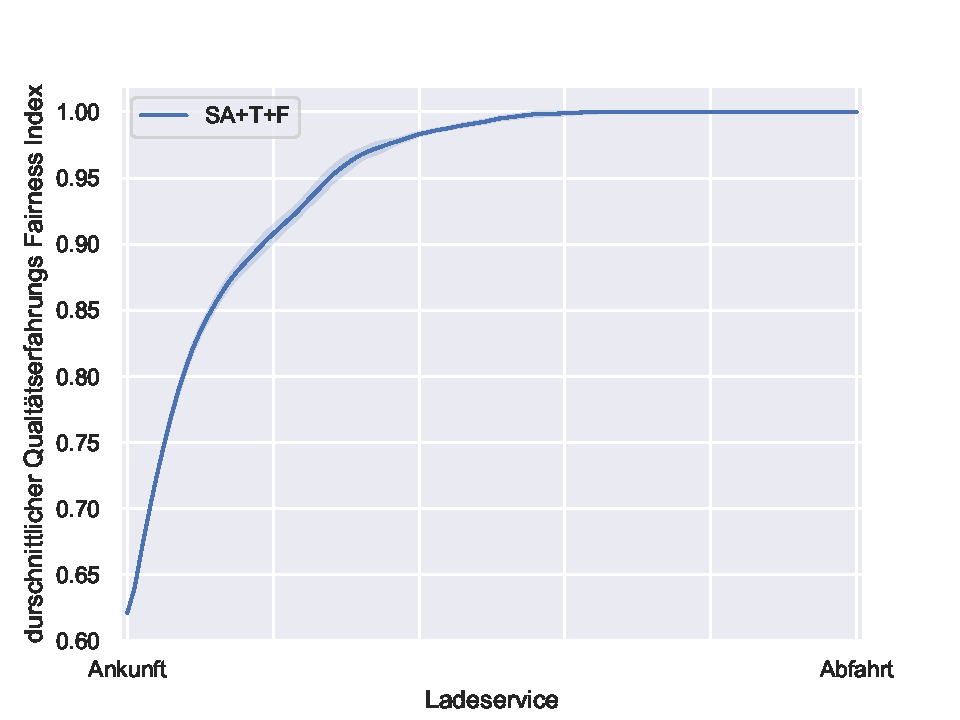
\includegraphics[scale=0.45]{img/SA_wT/SlottedAloha_waitingTime_VDE_tau_6_qoe.pdf}
	\caption{Durchschnittlicher Qualitätserfahrungs Fairness Index eines Elektrofahrzeuges über den Verlauf eines Ladeservices bei Verwendung der Methodik SA+T+F}
	\label{Abb_SAwTFairness}
\end{figure}

Abbildung \ref{Abb_SAwTFairness} zeigt den Fairness Index der jeweiligen Qualitätserfahrung mit Standardabweichung über den Zeitverlauf der Ladeservices. Die geringe Standardabweichung deutet auf ähnliche Ergebnisse über die Durchläufe hinweg hin. Die nur teilweise auftretende Standardabweichung zeigt, das sich das Ende der meisten Ladevorgänge tatsächlich in diesem Bereich sammelt, da die Wartezeiten schnell Einfluss darauf nehmen wie zugig ein Teilnehmer laden kann. Die geringe Abweichung zum Ende zeigt das dieser Bereich nur von wenigen Teilnehmer benötigt wird, welche sich allerdings über alle Durchläufe hinweg sehr gleich verhalten.

\subsection{VDE-Controller mit Transformatorkontroller}
\label{chap_VDE_t}
Eine weitere betrachtete Methodik ist der VDE-Kontroller, welcher an sich nur ein Spannungskontroller ist, hier aber um den in dieser Arbeit entwickelten Transformatorkontroller erweitert wurde. Für diese Kombination musste der mit dem Transformatorkontroller bereits rekonfigurierte Lag-Filter nochmals geändert werden. Diese erneute Änderung war nötig, da bei Verwendung des angedachten Lag-Filters  die Werte der Spannung an einem Punkt im simulierten Zeitraum so stark gefallen sind, dass PyPower nicht mehr in der Lage war diese Werte zu berechnen. Bei der Verwendung des Lag-Filters, wie er ursprünglich in Kapitel \ref{capBody:VDE} eingeführt wurde, trat dieses Problem nicht auf und die Simulation konnte erfolgreich beendet werden. 
\begin{figure}
	\begin{subfigure}{\linewidth}
		\includegraphics[scale=0.45]{img/VDE_tau_trafo/TrafoLast3.pdf}
		\caption{Transformatorlast über den Verlauf eines Tages}
		\label{Abb_VDETrafo_TrafoLast}
	\end{subfigure}
	\begin{subfigure}{\linewidth}
		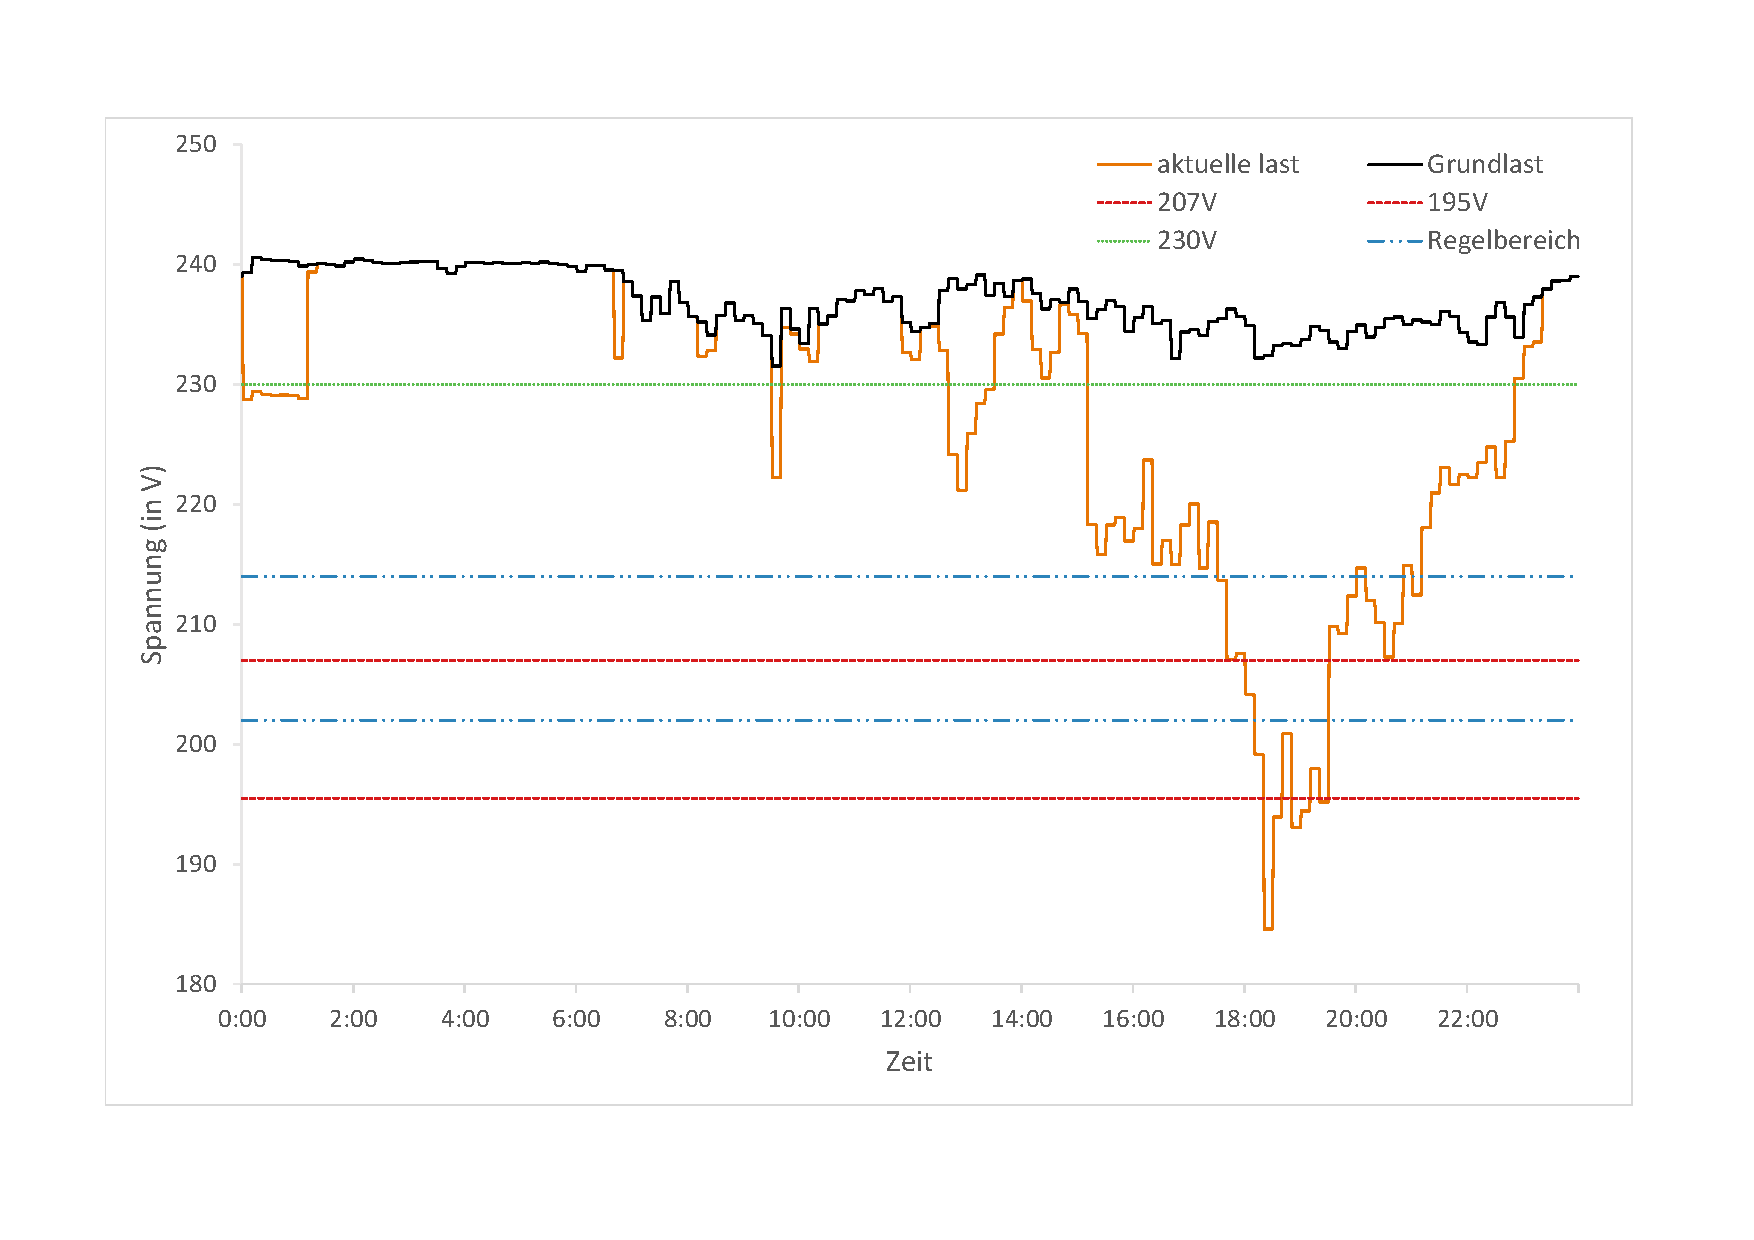
\includegraphics[scale=0.45]{img/VDE_tau_trafo/Spannung3.pdf}
		\caption{10 Minuten Mittelwerte der Spannung über den Verlauf eines Tages}
		\label{Abb_VDETrafo_Spannung}
	\end{subfigure}
	\caption{Transformatorlast und Spannungsverlauf bei Verwendung von VDE+Tr}
\end{figure}

In Abbildung \ref{Abb_VDETrafo_TrafoLast} ist die Menge der Scheinleistung dargestellt, welche vom Transformator ans Niederspannungsnetz abgegeben wird. Bei dieser Methodik werden keine Wartezeiten bestimmt, daher waren bei dieser Methodik keine mehrfachen Durchläufe nötig, somit gibt es auch keine Standardabweichung. Der Verlauf des Graphen zeigt, dass der verwendet Transformatorkontroller nur bedingt bzw. nicht den angedachten Zweck erfüllt. Auch nach der Veränderung des Lag-Filters ist bei dieser Methodik nicht gelungen, die Transformatorlast zu kontrollieren und so zu limitieren. Der Graphen hat große Ähnlichkeit mit dem Ergebnis des VDE-Kontrollers ohne die Erweiterung des Transformatorkontrollers, auch das weist daraufhin, dass der Transformatorkontroller seinen Zweck nicht erfüllen kann. \\
In Abbildung \ref{Abb_VDETrafo_Spannung} sind die Spannungswerte in 10 Minuten Intervallen enthalten, abbgebildet wird der minimal Wert über das gesamte Netz des jeweiligen Zeitpunktes.
Auch in dieser Abbildung ist der Regelbereich des Spannungskontrollers abgebildet. Ebenso wie bereits beim Transformatorkontroller muss hier allerdings festgestellt werden, dass der Spannungskontroller nicht ordentlich arbeitet, da die Werte nicht im oder über dem Regelbereich gehalten werden können. Das schnelle Absinken der Spannungswerte zeigt auch , dass der verwendete Kontroller aufgrund der Menge an bezogener Last nicht ausreicht.
\begin{figure}[htb]
\centering
	\includegraphics[scale=0.45]{img/VDE_tau_trafo/Teilnehmer3.pdf}
	\caption{Teilnehmerzahlen bei Verwendung von VDE+Tr über den Verlauf eines Tages}
	\label{Abb_VDETrafo_Teilnehmer}
\end{figure}

Abbildung \ref{Abb_VDETrafo_Teilnehmer} zeigt die Anzahl der ladebereiten und tatsächlich ladenden Teilnehmer an. Der geringe Abstand der beiden Kurven liegt an dem Fehlen von Wartezeiten bei dieser Methodik, welche Teilnehmer vom Laden abhalten würden. Die Abweichungen der beiden Graphen sind der Funktionsweise der Kontroller geschuldet, welche bei Unter- bzw. Überschreitung des jeweiligen Regelbereichs den Leistungsbezug unterbinden, dies allerdings nur für das jeweils aktuelle Zeitintervall. 
In dem Zeitraum von 0:00 Uhr bis etwa 15:00 Uhr befinden sich die Werte der Transformatorauslastung nur kurz im Regelbereich,während die Spannungswerte in dieser Zeitspanne gar nicht in den Regelbereich abfallen. Ab 15:00 Uhr nähern sich die Werte der Transformatorauslastung und der Spannung dem Regelbereich zunächst nur an, was sich auf die steigende Zahl der Teilnehmer zurückführen lässt. Ab ca. 16:00 Uhr nimmt die Zahl der Teilnehmer zuerst schnell zu, was in einem starken Abfall der Spannung und einer aufgrund starker Schwankungen nur teils hohen Transformatorlast endet. Mit einem Fallen der Teilnehmerzahl ab etwa 19:00 Uhr, erholen sich auch die Spannungswerte und die Transformatorauslastung wieder. Bis zu diesem Zeitpunkt war allerdings weder der Transformatorkontroller noch der Spannungskontroller in der Lage seinen angedachten Zweck zu erfüllen.
Aufgrund des fehlendem Effekts des Spannungskontroller konnte schon an dem einem betrachtetem Tag, die Einhaltung der Norm DIN EN 50160 nicht erreicht werden. Der Schwellenwert von -10 \% p.u. wird bei mindesten einem Teilnehmer bis zu 17 Mal unterschritten, was noch innerhalb des erlaubten Bereiches von etwa 50 Unterschreitungen liegt liegt, allerdings wird auch der Grenzwert von -15 \% p.u. unterschritten. Aufgrund von Unterschreitungen des Schwellenwerts bei -15 \% p.u. ist die Norm nicht erfüllt.
Bei dieser Methodik wird zwar sowohl der Spannungskontroller, als auch der Transformatorkontroller verwendet, jedoch werden keinerlei Wartezeiten bestimmt, mit denen auf möglicherweise aufgetreten Kollisionen reagiert werden könnte. Es wurden über den simulierten Zeitraum von einer Woche 1882 Situationen festgestellt, in denen eine zu niedrige Spannung gemessen wurde, und 5946 Situationen in denen eine zu hohe Auslastung des Transformators festgestellt wurde. Insgesamt kam es zu 5964 Situationen, in denen eine Wartezeit hätte bestimmt werden können, da dies bei dieser Methodik allerdings nicht vorgesehen ist, wurden keine Wartezeiten berechnet.
Alle im betrachteten Simulationszeitraum gestarteten Ladeservice wurden erfolgreich abgeschlossen, nicht ein Fahrzeug musste die Ladestation mit einem Ladestand von weniger als 100 \% verlassen. Da alle Ladeservice erfolgreich abgeschlossen wurden, ist die Qualität der Ladeservice maximal.
\begin{figure}
	\begin{subfigure}{0.49\linewidth}
		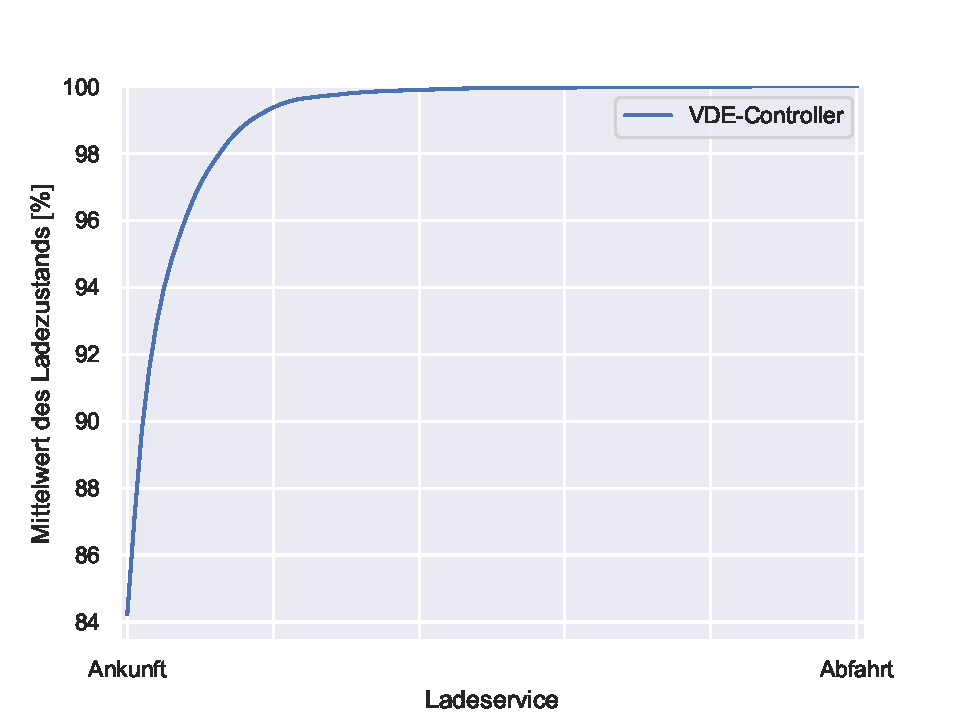
\includegraphics[width=\linewidth]{img/VDE_tau_trafo/tau_VDE_trafo_2_soc_mean.pdf}
        \subcaption{Durchschnittlicher Ladezustand aller Elektrofahrzeuges über den Verlauf eines Ladeservices}
        \label{ABB_VDETrafo_SocMEAN}
	\end{subfigure}
	\begin{subfigure}{0.49\linewidth}
		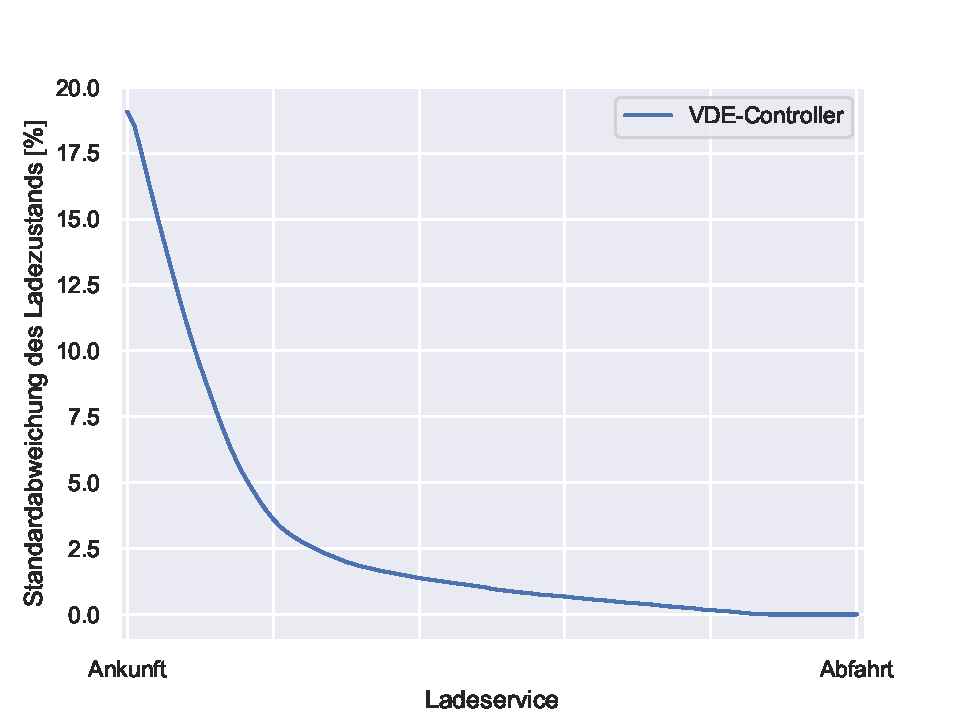
\includegraphics[width=\linewidth]{img/VDE_tau_trafo/tau_VDE_trafo_2_soc_std.pdf}
        \subcaption{Durschschnittliche Standardabweichung des Ladezustandes aller Elektrofahrzeuges über den Verlauf eines Ladeservices}
        \label{ABB_VDETrafo_SocSTD}
	\end{subfigure}
	\caption{Durchschnittlicher Ladezustand mit Standardabweichung bei Verwendung der Methodik SA+T+F}
\end{figure}
Abbildung \ref{ABB_VDETrafo_SocMEAN} zeigt dem mittleren Ladestand aller Teilnehmer über den zeitlichen Verlauf der jeweilige Ladeservice. Abbildung \ref{ABB_VDETrafo_SocSTD} zeigt die zugehörige Standardabweichung des Ladestandes ebenfalls über den zeitlichen Verlauf der Ladeservice hinweg. Der schnelle Anstieg des mittleren Ladestandes deutet daraufhin das die Fahrzeuge schnell mit größeren Mengen an Energie versorgt werden können. Die Standardabweichung fällt in ebensolchem Tempo, was den Schluss zulässt, dass viele Fahrzeuge mit ihrem ladestand nahe am Mittelwert liegen. Der schnelle Anstieg auf einen Wert, nahe dem Zielwert, zeigt das viele Fahrzeuge in der Lage sind bereits zu Beginn des Ladeservices das Ziel zu erreichen oder ihm nahe zu kommen. Das Abnehmen der Standardabweichung verlangsamt sich, als diejenigen Fahrzeuge, welche nicht viel Energie laden musste, fertig geladen haben. Die Fahrzeuge, welche diesen Zeitabschnitt ihres Ladeservice noch zum laden benötigen starteten mit einem niedrigen Ladestand in den Ladeservice und brauchen daher eine gewisse Zeit um einen Ladezustand von 100 \% zu erreichen. Diese Tatsache zeigt, dass es trotz der schnellen Abnahme der Standardabweichung dennoch verhältnismäßig lange dauert, bis die Ladeservice als erfolgreich eingestuft werden können.
\begin{figure}[htb]
\centering
	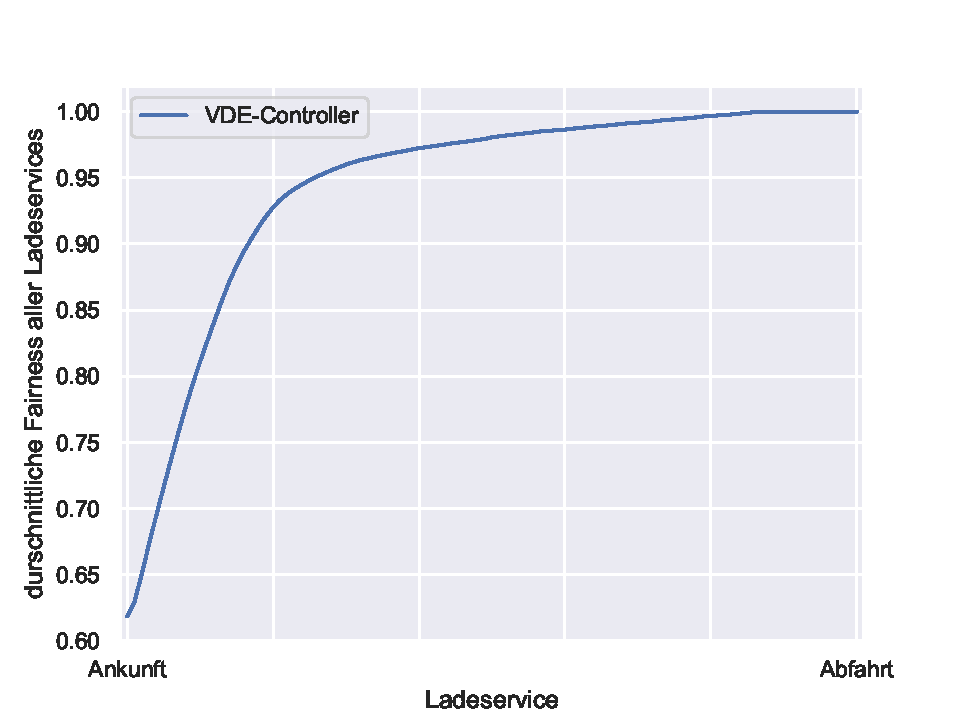
\includegraphics[scale=0.45]{img/VDE_tau_trafo/tau_VDE_trafo_2_qoe.pdf}
	\caption{Durchschnittlicher Qualitätserfahrungs Fairness Index aller Elektrofahrzeuges über den Verlauf eines Ladeservices bei Verwendung der Methodik VDE+Tr}
	\label{Abb_VDETrafo_Fairness}
\end{figure}

Abbildung \ref{Abb_VDETrafo_Fairness} zeigt den mittlere Fairness Index der Qualitätserfahrung aller Teilnehmer über den zeitlichen Verlauf ihrer Ladeservice hinweg. Wie bereits die Standardabweichung zeigt dieser Graph einen schnellen Anstieg zu Beginn, dann flacht die Kurve jedoch ab und erst nahe am Ende der Ladeservice wird die maximal mögliche Fairness erreicht. Dieser Verlauf der Kurve weist darauf hin, dass es vielen Teilnehmer gelingt bereits zu Beginn ihres Ladeservices einen hohen Ladestand zu erreichen, es jedoch auch Teilnehmer gibt, welche sehr viel ihrer Zeit nutzen müssen um einen hohen Ladestand zu erreichen, dies zeigt wieder Unterschiede zwischen den Fahrzeugen auf.

\subsection{Slotted Aloha mit Teilnehmerzahl mit Transformatorkontroller}
\label{chap_SAparT}
Die Methodik, welche den VDE-Kontroller mit der Teilnehmer basierten Slotted ALOHA Regelung erweitert, wurde bereits betrachten. Hier werden die Ergebnisse vorgestellt, wird zusätzlich noch der Transformatorkontroller verwendet.
\begin{figure}
	\begin{subfigure}{\linewidth}
		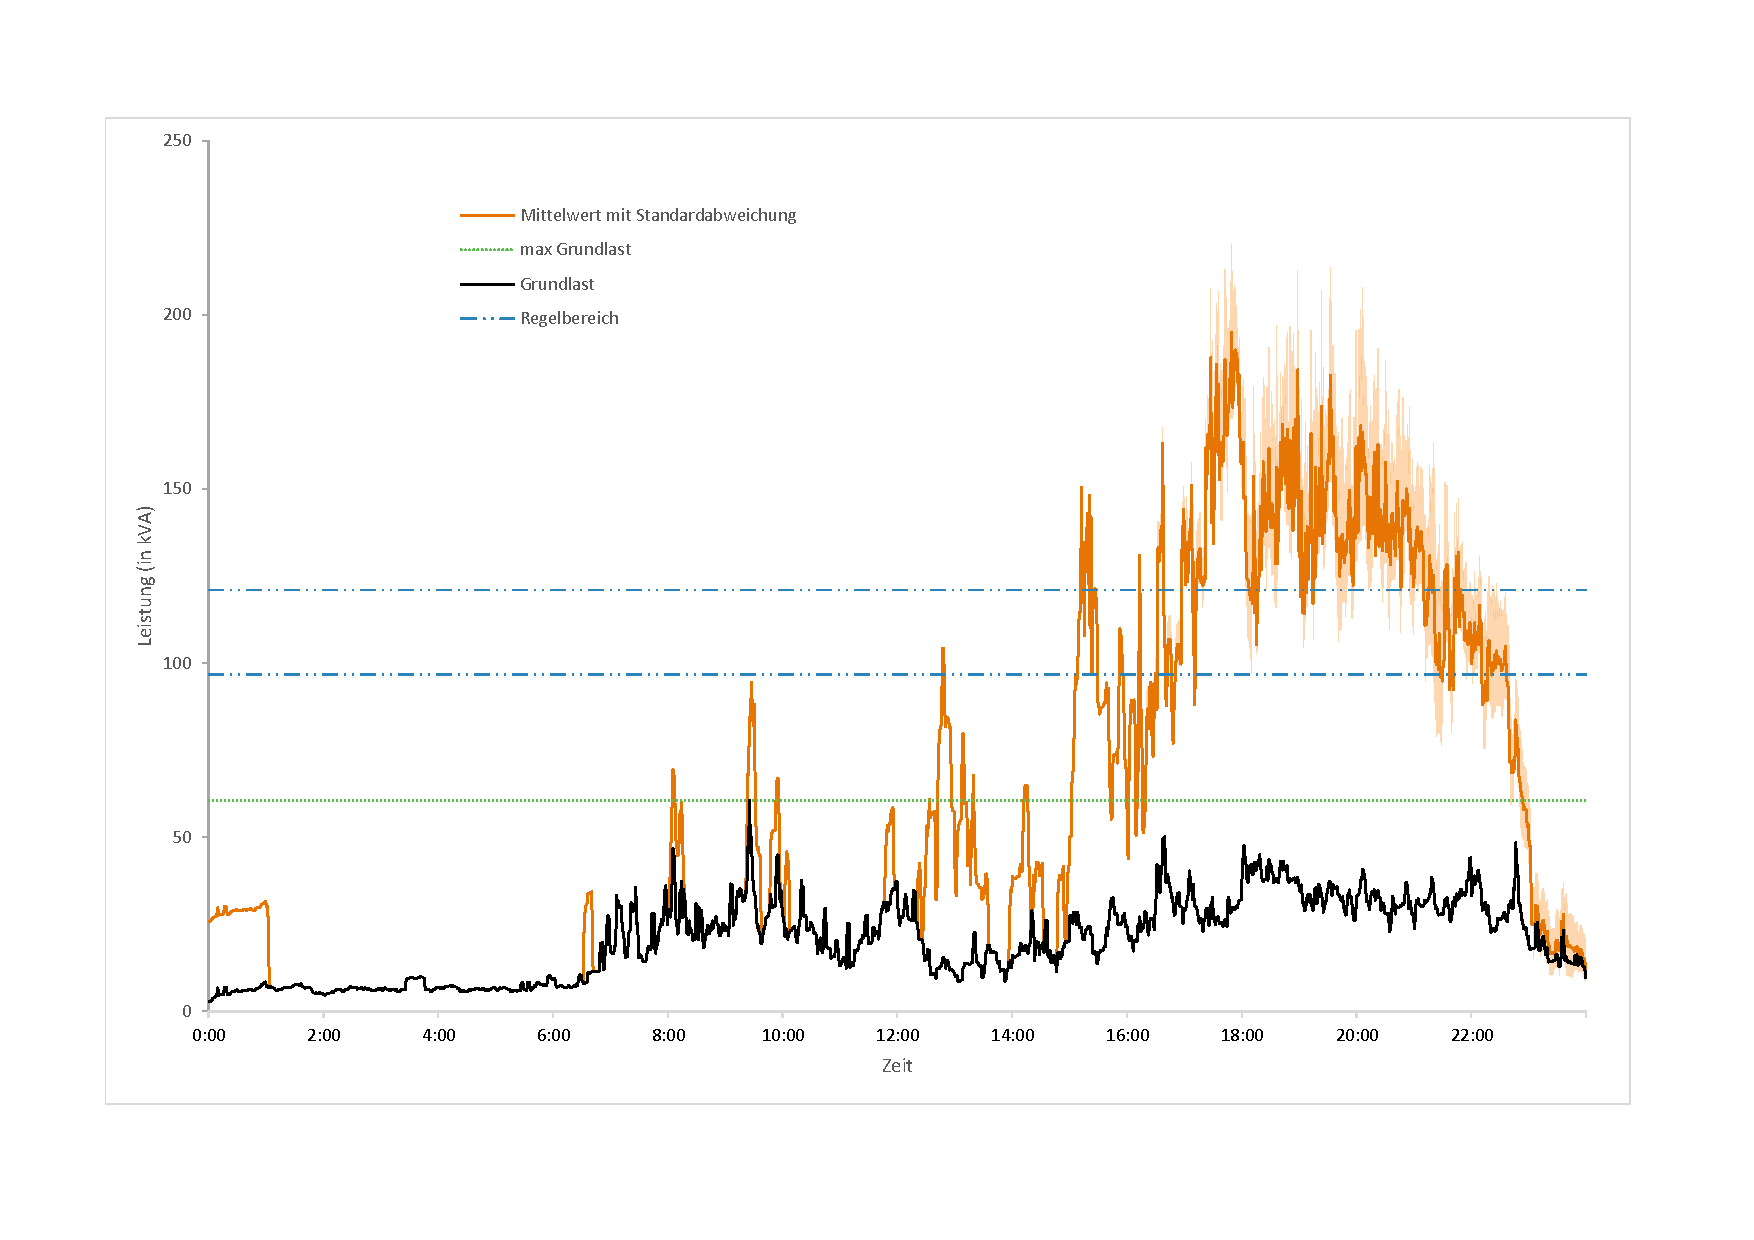
\includegraphics[scale=0.45]{img/SA_par_trafo/TrafoLast4.pdf}
		\caption{Transformatorlast über den Verlauf eines Tages}
		\label{Abb_SAparTrafo_TrafoLast}
	\end{subfigure}
	\begin{subfigure}{\linewidth}
		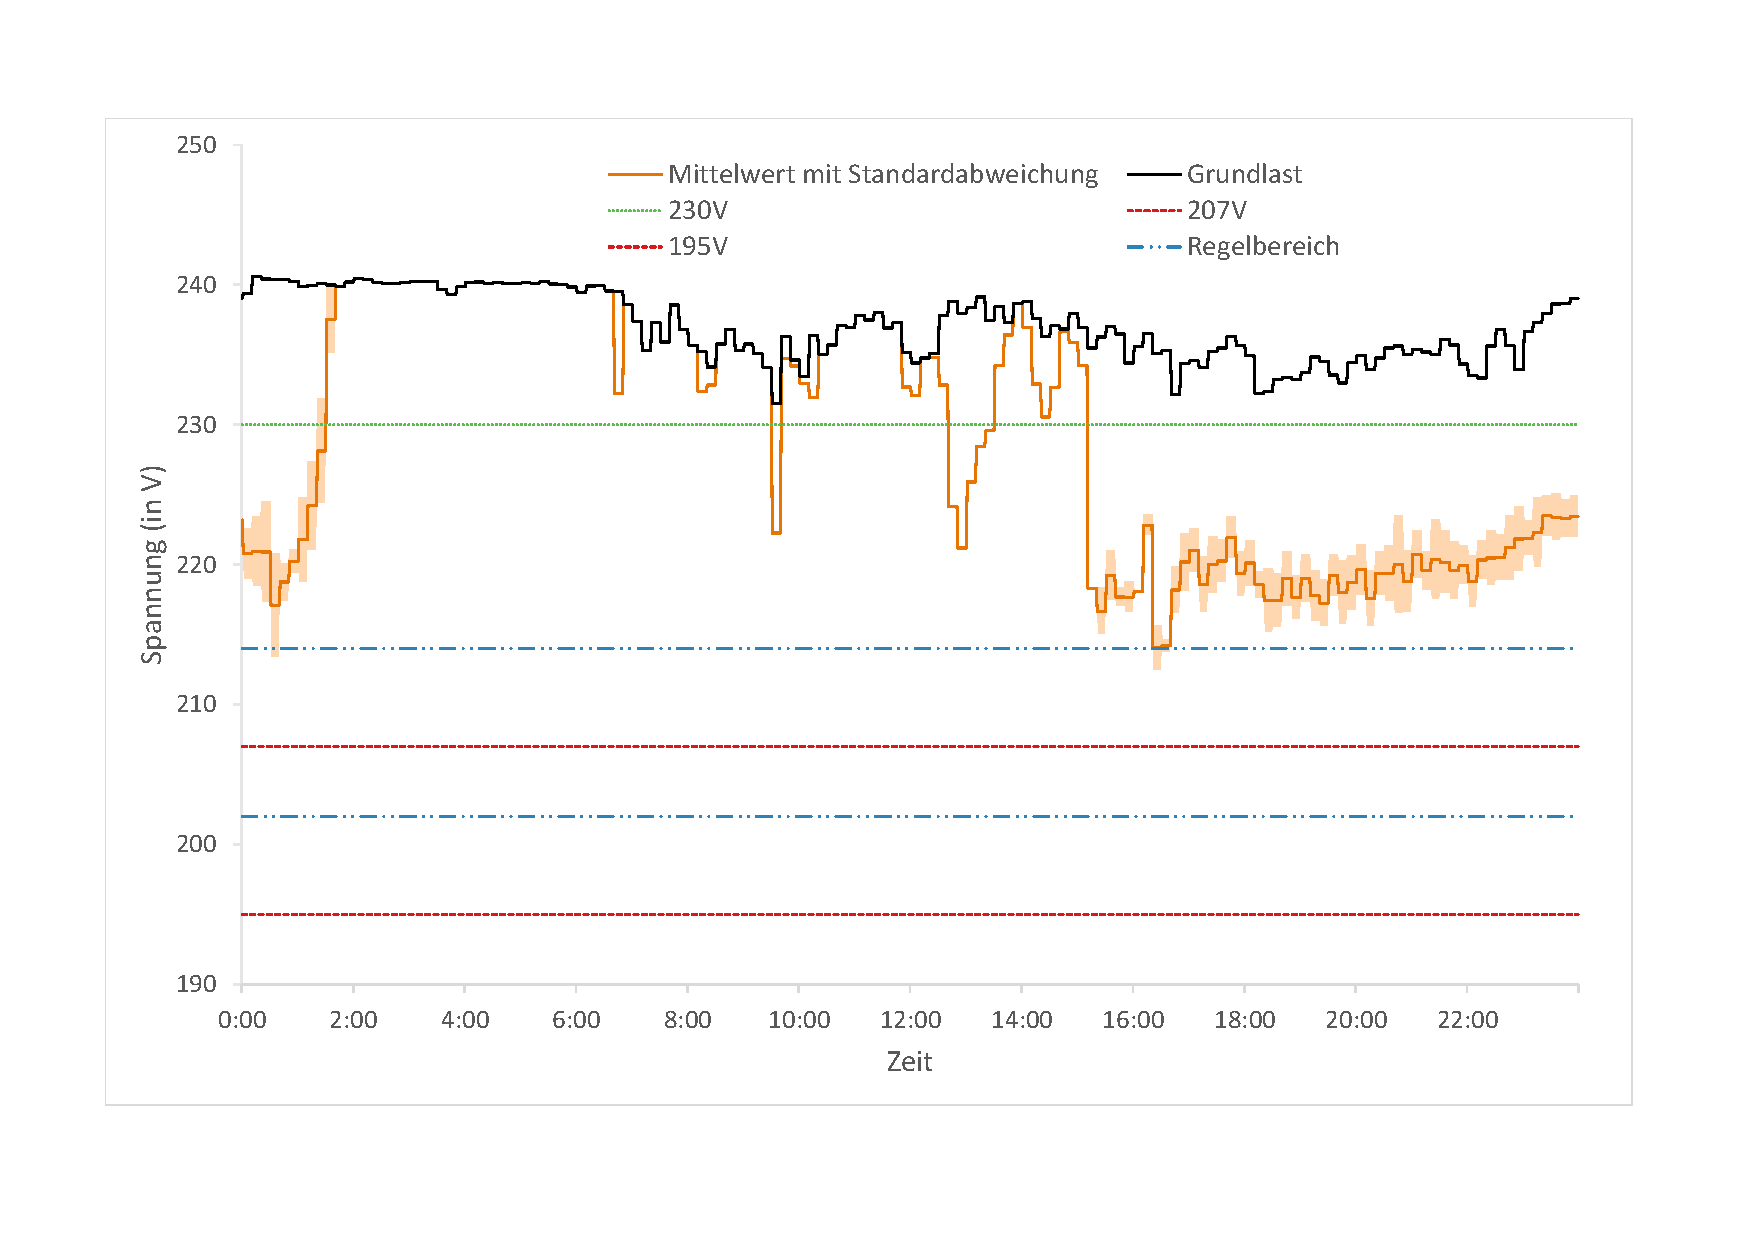
\includegraphics[scale=0.45]{img/SA_par_trafo/Voltage3.pdf}
		\caption{10 Minuten Mittelwerte der Spannung über den Verlauf eines Tages}
		\label{Abb_SaparTrafo_Spannung}
	\end{subfigure}
	\caption{Transformatorlast und Spannungsverlauf bei Verwendung von SA+T+Tr}
\end{figure}

Abbildung \ref{Abb_SAparTrafo_TrafoLast} zeigt den Mittelwert der Menge der bezogenen Scheinleistung am Transformator mit der zugehörigen Standardabweichung über den Verlauf eines Tages. Die hier betrachteten Methodik verwendet den Transformatorkontroller, welcher innerhalb der markierten Grenzen arbeitet und bei Messwerten oberhalb des Regelbereiches keinen weiteren Lastbezug zulässt. Am Graphen ist erkennbar wie der Kontroller einen dauerhaften Bezug von mehr als der erlaubten Leistung unterbindet und sich der Mittelwert meist innerhalb des Regelbereiches oder darunter aufhält. Einzelne Spitzen nach oben sind aufgrund der dezentralen Verwendung des Kontrollers nicht zu vermeiden, da die einzelnen Teilnehmer die anderen Teilnehmer nicht berücksichtigen. Die Last bleibt, wenn sie sich im Regelbereich befindet, stabil und schwankt verhältnismäßig. Die teils hohe Standardabweichung weist auf große Unterschiede zwischen den absolvierten Durchläufen hin.  \\
Abbildung \ref{Abb_SaparTrafo_Spannung} zeigt die Minimalwerte der Mittelwerte der 10 Minuten Intervalle der Spannung über alle Anschlusspunkte hinweg. Neben den eigentlichen Werten wird auch die Standardabweichung über die durchlaufenen Durchgänge mitabgebildet. Im Vergleich zur Transformatorlast, weist die Standardabweichung hier auf eine höhere Ähnlichkeit der einzelnen Durchläufe hin. Je weiter sich die Messwerte allerdings von der Grundlast entfernen , desto größer wird die Standardabweichung. Anhand des Verlaufs des Graphens ist erkennbar, dass die dargestellten Werte nur an wenigen Punkten bis in den Regelbereich des Kontrollers vordringen. Da nur wenige Werte innerhalb des Regelbereiches liegen, kann der Spannungskontroller auch nur wenig Einfluss nehmen.\\
\begin{figure}[htb]
\centering
	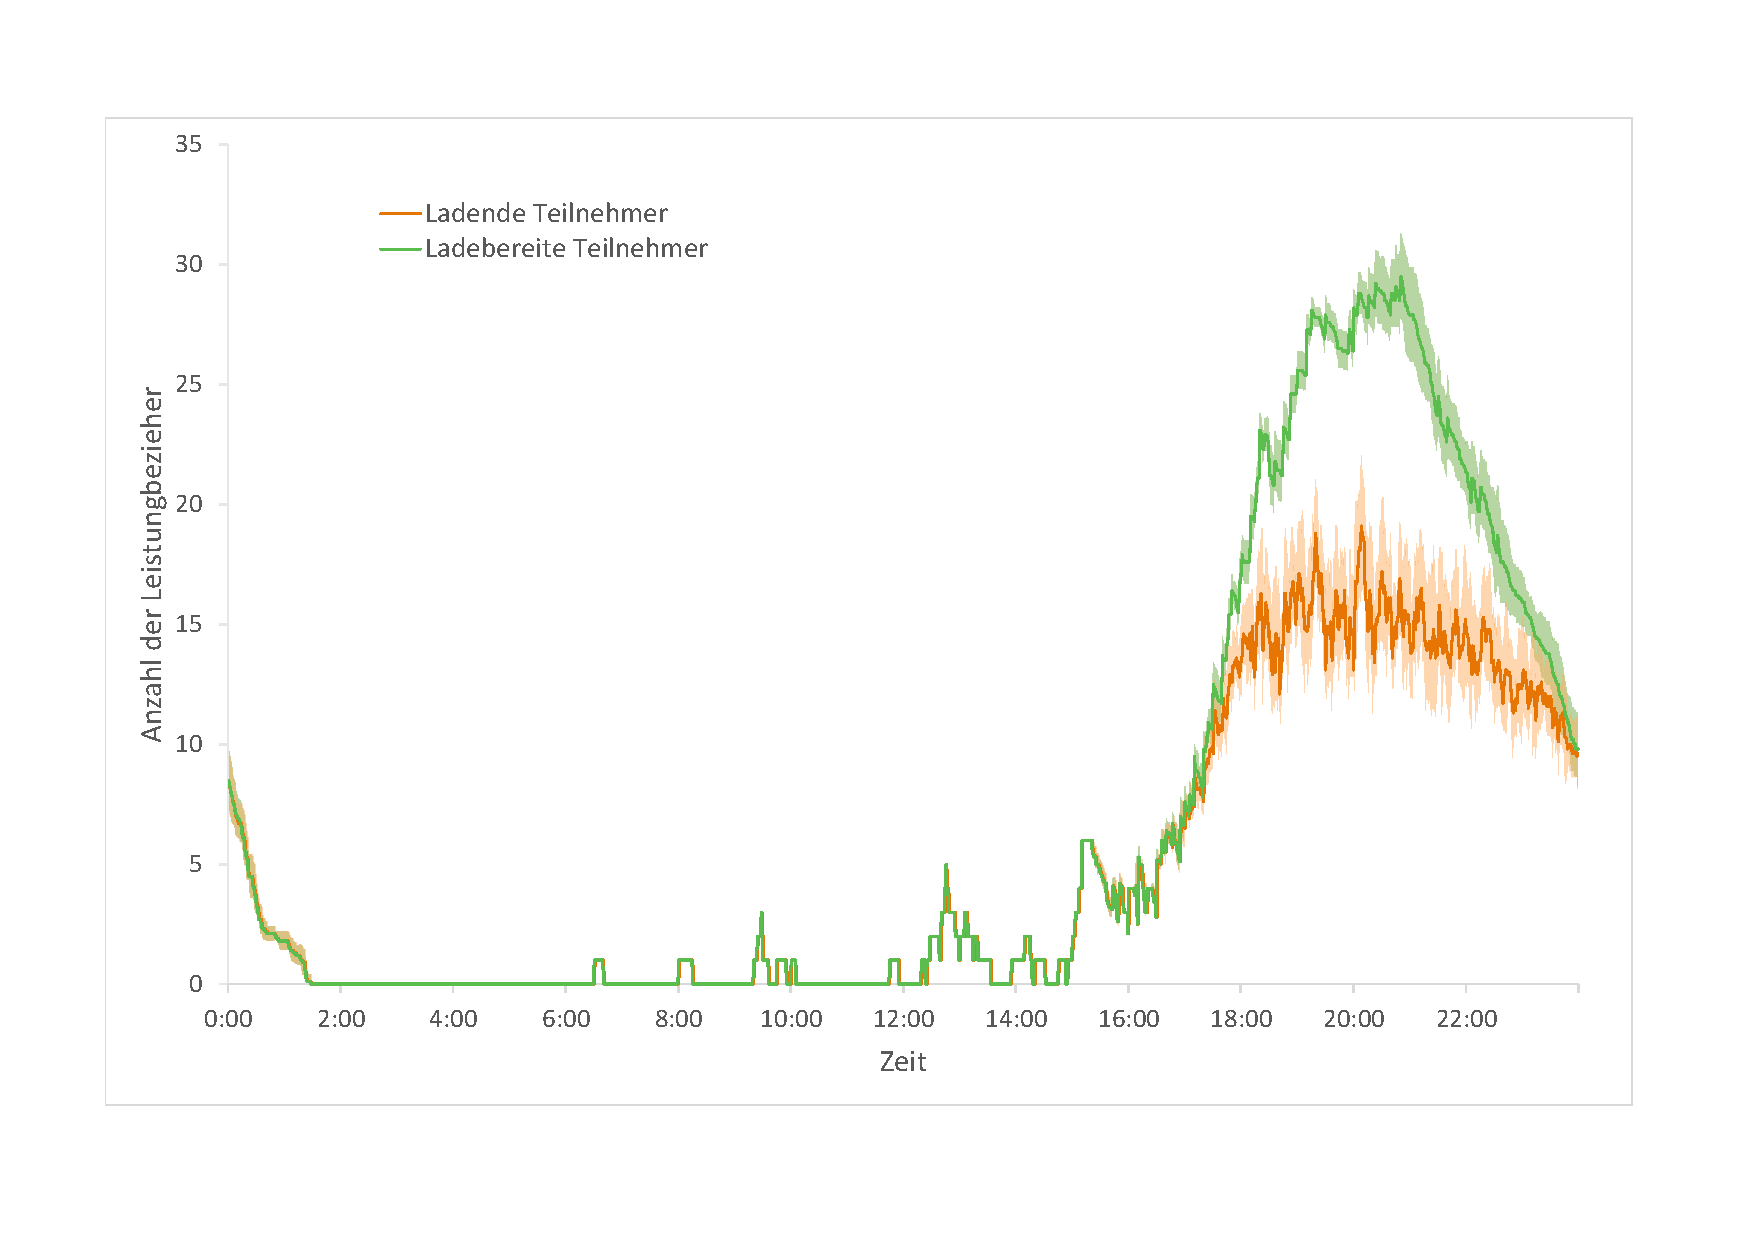
\includegraphics[scale=0.45]{img/SA_par_trafo/Teilnehmer4.pdf}
	\caption{Teilnehmerzahlen bei Verwendung von SA+T+Tr über den Verlauf eines Tages}
	\label{Abb_SAparTrafo_Teilnehmer}
\end{figure}
In Abbildung \ref{Abb_SAparTrafo_Teilnehmer} sind die Mittelwerte und Standardabweichung der Anzahl der ladebereiten und der tatsächlich ladenden Teilnehmer abgebildet. Die Differenz zwischen der Anzahl an ladebereiten und tatsächlich ladenden Teilnehmern kommt durch das Einhalten der nach einer Kollision berechneten Wartezeit zustande. Die teils schnellen Anstiege der Zahl der ladenden Teilnehmer ohne denselben Anstieg in der Zahl der ladebereiten Teilnehmer weist auf zu ähnliche Wartezeiten hin. Diese zu ähnlichen Wartezeiten helfen der Lastverteilung, die durch das Warten erreicht werden soll, nur bedingt und sollten eigentlich vermieden werden. Da bei dieser Methodik zur Bestimmung der Wartezeit allerdings nur die Zahl der ladebereiten Teilnehmer verwendet wird, gibt es nur sehr beschränkte Auswahlmöglichkeiten und damit auch Überscheidungen bei der Auswahl.\\
Zu Beginn des betrachteten Zeitraumes befinden sich bereits Teilnehmer in ihren Ladeservices, was auch die Transformatorauslastung und die Spannungswerte erklärt. Die Teilnehmer schließen die Ladeservice allerdings schnell ab, was die Transformatorlast und die Spannung, auf die Grundlast zurückkommen lasst. In dem Zeitraum von 02:00 Uhr bis etwa 15:00 Uhr steigen die Werte zwar gelegentlich an, allerdings ist weder das Eingreifen des Transformatorkontrollers noch das des Spannungskontrollers erforderlich. Ab etwa 15:00 Uhr steigt die Zahl der ladebereiten Teilnehmer schnell an, was sich auch an der Höher der Transformatorlast und dem Fallen der Spannung erkennen lässt. Ab etwa 18:00 Uhr beginnt sich ein deutlicher Unterschied zwischen der Anzahl an ladebereiten Teilnehmer und tatsächlich ladenden Teilnehmern zu zeigen. Die Anzahl der ladenden Teilnehmer hört bei etwa 20 Teilnehmer auf zu steigen, während die Anzahl der ladebereiten Teilnehmer auf mehr als 30 ansteigt. Die eher stabile Zahl an ladenden Teilnehmer zeigt sich auch an der stabilen Transformatorauslastung und den stabilen Messwerten der Spannung. Zum Ende des betrachteten Zeitraumes sinkt Anzahl der Teilnehmer und so sinkt auch die Transformatorlast und die Spannung nähert sich wieder der Grundlast an.\\
Auch für diese Methodik wird die Einhaltung der Norm DIN EN 50160 in Hinsicht auf die Spannungsqualität an Anschlusspunkten des Niederspannungsnetzes untersucht. Im Schnitt über alle Durchgänge mit dieser Methodik wurden keine Unterschreitungen von -10~\% p.u. und keine Unterschreitungen der -15~\% p.u. Marke festgestellt. Somit wurde die Norm erfüllt.
Da hier sowohl der Transformator- als auch der Spannungskontroller verwendet wurde, wird bei dieser Methodik auch auf beide Arten von Kollisionen reagiert. Im Schnitt kam es zu 461,8 ($\pm$ 10,4~\%) Spannungskollisionen und zu 6588,7 ($\pm$ 1,6~\%) Transformatorkollisionen. Da die Kollisionen auch gemeinsam auftreten können, kam es nur in 6589,3 ($\pm$ 1,6~\%) Fällen zu einer Situation in der eine oder beide Kollisionsarten vorlagen. Unterbrechungen von Ladevorgängen durch Kollisionen gab es lediglich in 3084,0 ($\pm$ 0,7 \%) Fällen. Das bedeutet in weniger als der Hälfte der Fälle; wo eine Kollision aufgetreten ist, musste auch darauf reagiert werden.\\
In dem betrachteten Simulationszeitraum von einer Woche wurden 557 Ladeservices gestartet, es konnten allerdings im Schnitt nur 554,1 Services erfolgreich abgeschlossen werden, also mussten durchschnittlich 2,9 Mal ($\pm$ 42~\%) Ladeservices beendet werden, bevor die Batterie des Fahrzeuges auf 100~\% geladen werden konnte. Die Standardabweichung des Ladestandes beim Verlassen der Ladestation lag nur bei etwa 0,43~\% ($\pm$~39,5~\%), der Mittelwert des Ladezustandes bleibt davon allerdings unverändert bei 100~\% wenn die Ladestation verlassen wird. Der Mittelwert und die Standardabweichung des Ladestandes sind in Abbildung \ref{ABB_SAparTrafo_SocMEAN} bzw. \ref{ABB_SAparTrafo_SocSTD} angetragen.\\
\begin{figure}
	\begin{subfigure}{0.49\linewidth}
		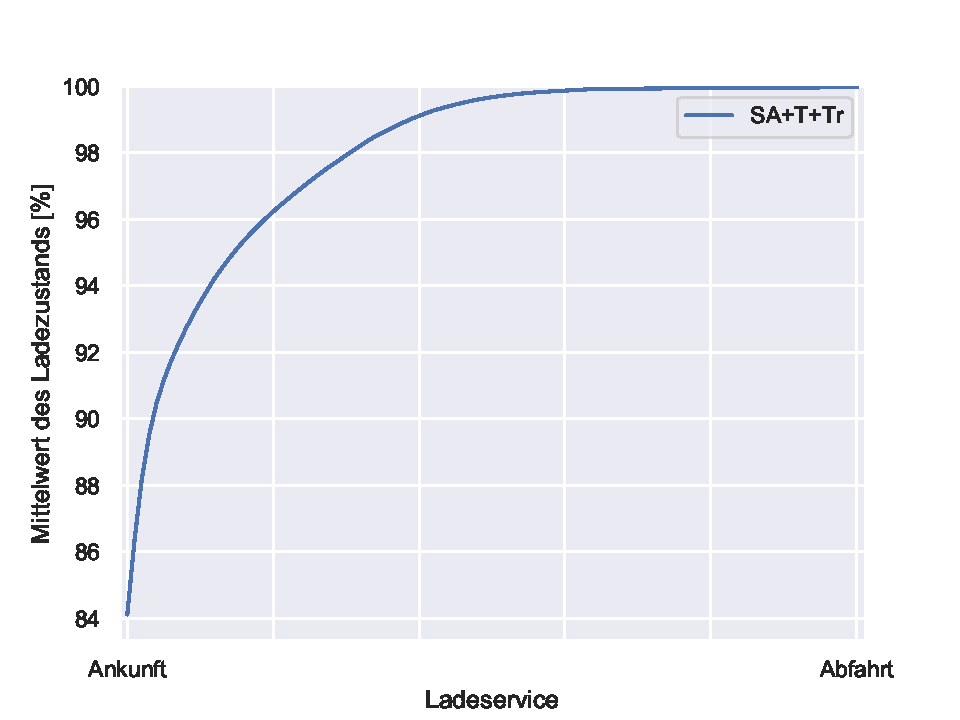
\includegraphics[width=\linewidth]{img/SA_par_trafo/SlottedAloha_participants_VDE_tau_trafo_15_soc_mean.pdf}
        \subcaption{Durchschnittlicher Ladezustand aller Elektrofahrzeuges über den Verlauf eines Ladeservices}
        \label{ABB_SAparTrafo_SocMEAN}
	\end{subfigure}
	\begin{subfigure}{0.49\linewidth}
		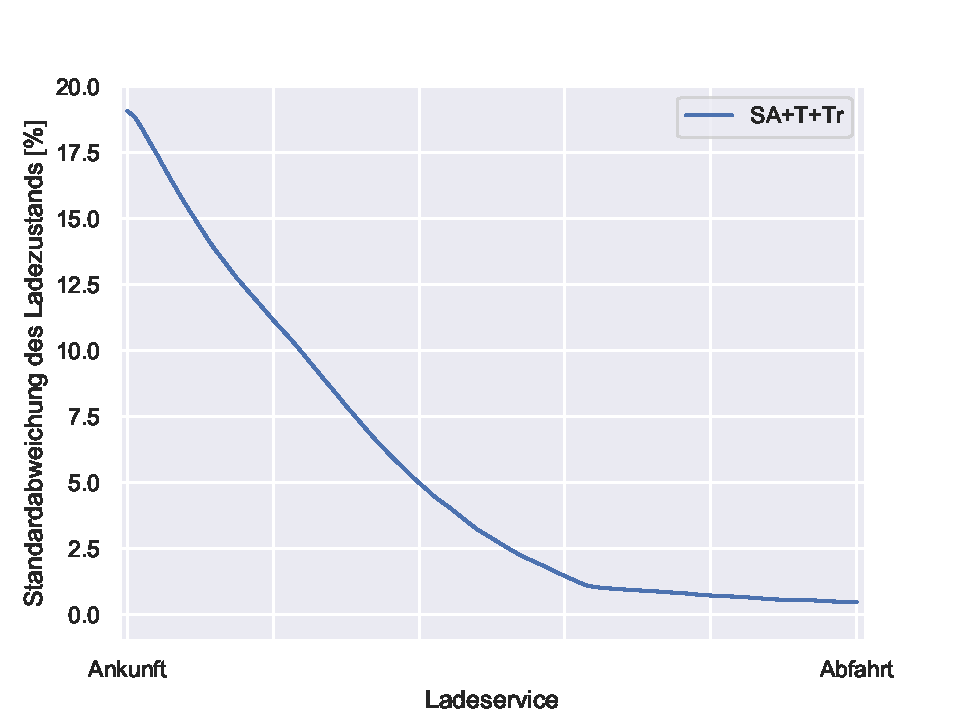
\includegraphics[width=\linewidth]{img/SA_par_trafo/SlottedAloha_participants_VDE_tau_trafo_15_soc_std.pdf}
        \subcaption{Durschschnittliche Standardabweichung des Ladezustandes aller Elektrofahrzeuges über den Verlauf eines Ladeservices}
        \label{ABB_SAparTrafo_SocSTD}
	\end{subfigure}
	\caption{Durchschnittlicher Ladezustand mit Standardabweichung bei Verwendung von SA+T+Tr}
\end{figure}
Abbildung \ref{ABB_SAparTrafo_SocMEAN} Zeigt den mittleren Ladestand aller Fahrzeuge über den zeitlichen Verlauf der Ladeservice hinweg. Abbildung \ref{ABB_SAparTrafo_SocSTD} zeigt die gemittelte Höhe der Standardabweichung des Ladezustandes über alle Ladeservices im zeitlichen Verlauf. Trotz der verbleibenden Standardabweichung zum Ende der Ladeservice hin, zeigt Abbildung \ref{ABB_SAparTrafo_SocMEAN} 100 \% mittleren Ladezustand an. Der Wechsel der  Abnahme der Standardabweichung bei etwa 60 \% der Zeit weisen daraufhin, das viele Ladevorgänge bis dahin abgeschlossen sind, die die es nicht sind allerdings nur noch sehr langsam ihren Ladestand erhöhen können. \\
\begin{figure}[htb]
\centering
	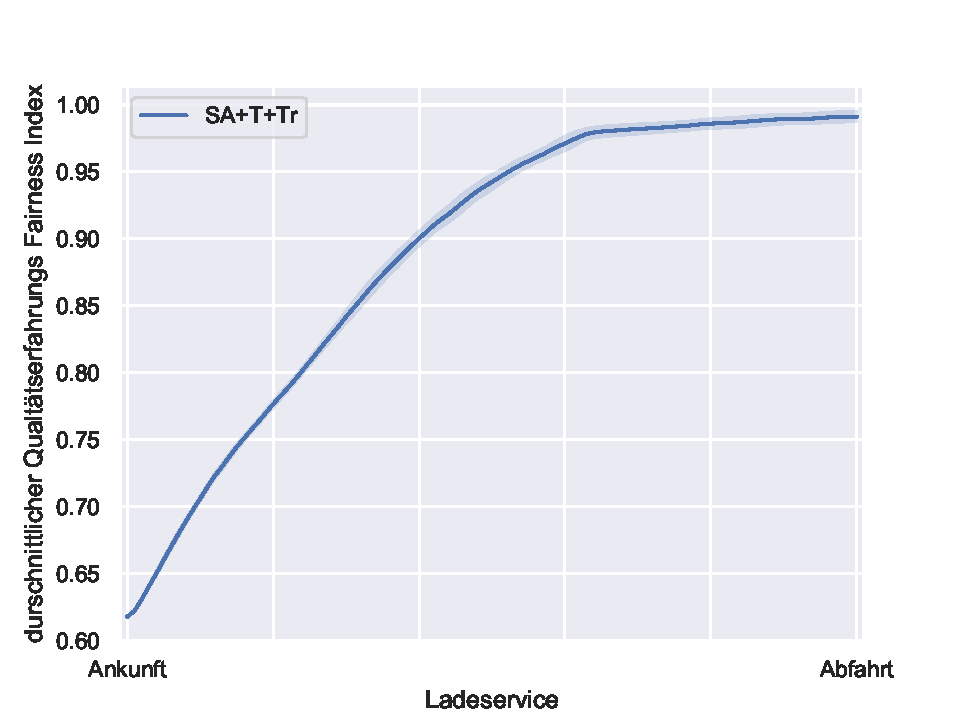
\includegraphics[scale=0.45]{img/Sa_par_trafo/SlottedAloha_participants_VDE_tau_trafo_15_qoe.pdf}
	\caption{Durchschnittlicher Qualitätserfahrung Fairness Index aller Elektrofahrzeuges über den Verlauf eines Ladeservices bei Verwendung der Methodik SA+T+Tr}
	\label{Abb_SAparTrafo_Fairness}
\end{figure}
Abbildung \ref{Abb_SAparTrafo_Fairness} zeigt den Mittelwert des Fairness Index über alle Teilnehmer hinweg. Die Fairness bestimmt sich über die Standardabweichung, da diese hier nicht 0 wird, wird auch die Fairness nicht maximal. Da nicht alle Teilnehmer in der Lage waren ihre Ladeservice erfolgreich abzuschließen, erreicht auch der Wert der Qualitätserfahrung nicht das Maximum, im Mittel über alle Durchläufe konnte eine Qualitätserfahrung von 0,99 von 1 erreicht werden. Die Fehlende Qualitätserfahrung spiegelt sich auch in der Fairness wider, welch zwar hoch wird, jedoch wird auch hier das Maximum nicht erreicht. Auch am Graphen der Fairness zeigt sich ein Bild wie bei der Standardabweichung des Ladestandes. Bis etwa 60 \% durch die Ladeservice steigt der Graph gleichmäßig an, ab dann steigt der Graph allerdings nur noch sehr gering weiter an. 

\subsection{Slotted Aloha mit Teilnehmerzahl und Fahrzeugparametern mit Transformatorkontroller}
\label{chap_SAwtT}
Die Methodik, welche bei der Erweiterung des VDE-Kontrollers um die Slotted Aloha Regelung neben der Teilnehmerzahl auch Fahrzeugparameter verwendet wurde ebenfalls noch um den Transformatorkontroller erweitert.
\begin{figure}
	\begin{subfigure}{\linewidth}
		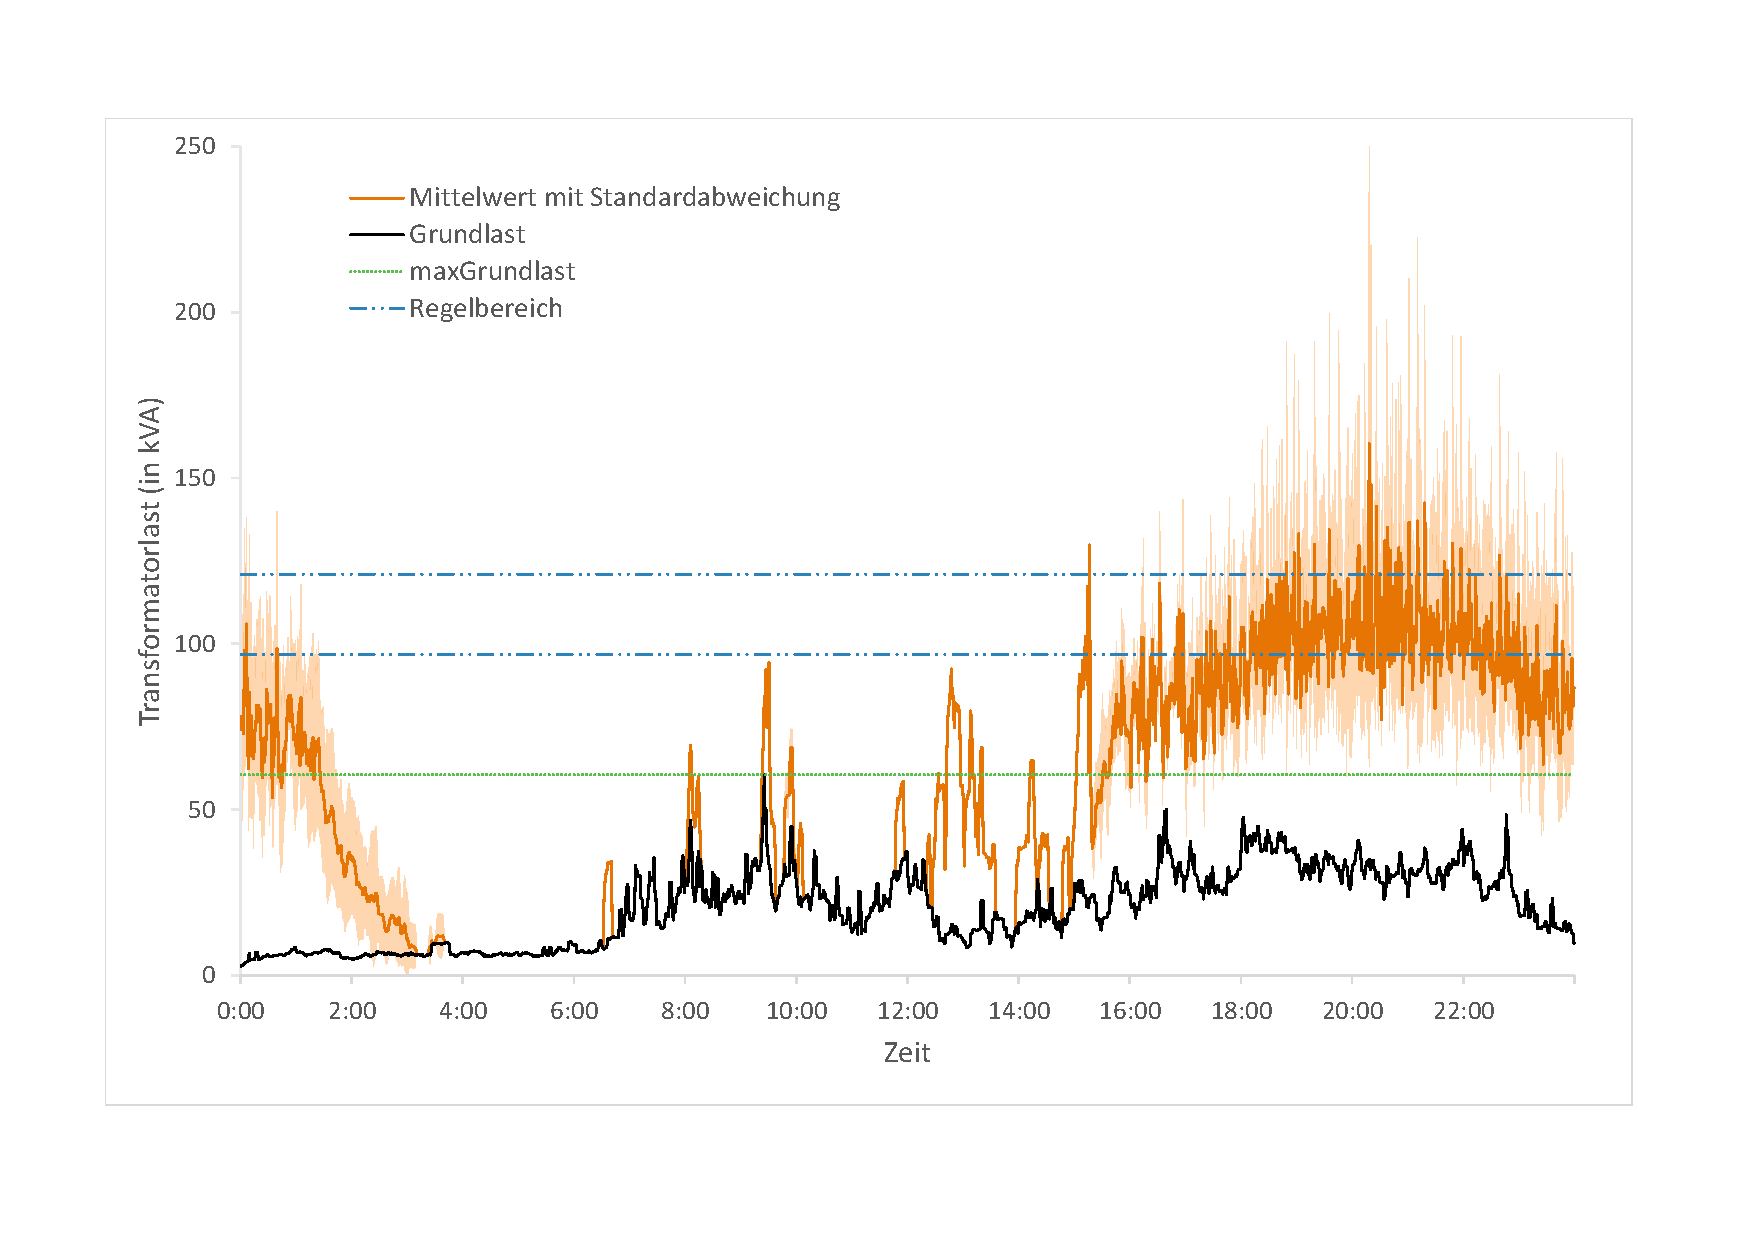
\includegraphics[scale=0.45]{img/SA_wT_trafo/TrafoLast2.pdf}
		\caption{Transformatorlast über den Verlauf eines Tages}
		\label{Abb_SAwtTrafo_TrafoLast}
	\end{subfigure}
	\begin{subfigure}{\linewidth}
		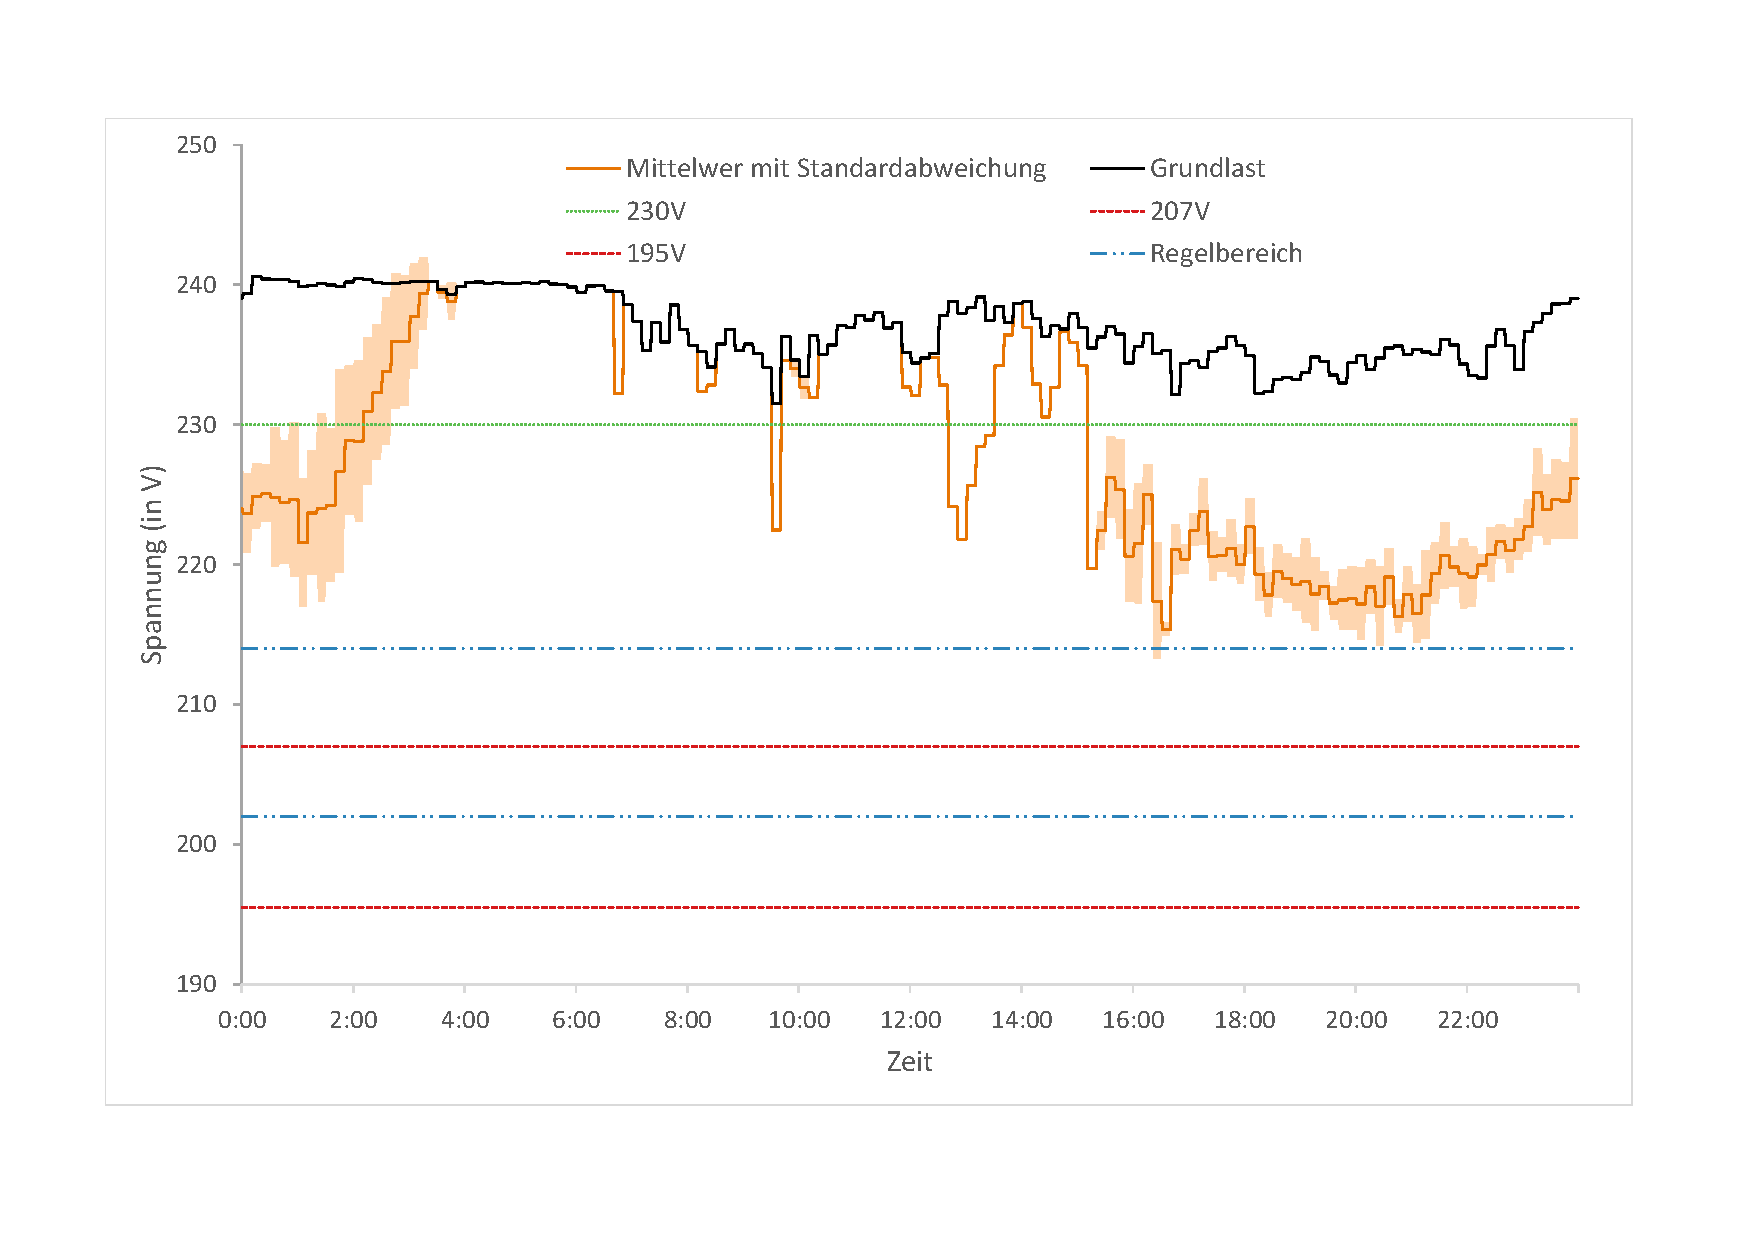
\includegraphics[scale=0.45]{img/SA_wT_trafo/Spannung2.pdf}
		\caption{10 Minuten Mittelwerte der Spannung über den Verlauf eines Tages}
		\label{Abb_SAwtTrafo_Spannung}
	\end{subfigure}
	\caption{Transformatorlast und Spannungsverlauf bei Verwendung von SA+T+F+Tr}
\end{figure}
Abbildung \ref{Abb_SAwtTrafo_TrafoLast} zeigt den Mittelwert der Scheinleistung, welche am Transformator ins Niederspannungsnetz abgegeben wurde, mit der dazugehörigen Standardabweichung über den Verlauf eines Tages. Auch hier wird der Transformatorkontroller verwendet, welcher innerhalb der markierten Grenzen arbeitet und bei Messwerten oberhalb des Regelbereiches keinen weiteren Lastbezug zulässt. Die teils hohe Standardabweichung deutet auf unterschiedliche Ergebnisse der einzelnen Durchläufe hin. Bis auf einige Ausbrüche nach oben, welche sich aufgrund des dezentralen Verhaltens des Kontrollers nicht vermeiden lassen, bleiben die Werte des Graphen im oder unter dem Regelbereich des Kontrollers. Wenn sich die Menge der bezogenen Leistung am oder im Lastbereich befindet, schwanken die Werte zwar, allerdings in einem vertretbaren den Umständen entsprechenden Rahmen.\\
In Abbildung \ref{Abb_SAwtTrafo_Spannung} sind die Mittelwerte der minimalen 10 Minuten Mittelwerte der Spannung angetragen, ebenso wie die zugehörige Standardabweichung. Die Werte weisen teils eine hohe Standardabweichung auf, was auf größere Unterschiede zwischen den einzelnen Durchläufen hindeutet. Wie bereits bei der vorhergehenden Methodik, welche ebenfalls den Trafokontroller verwendet, liegen kaum Werte innerhalb des Regelbereiches des Spannungskontrollers. Somit lässt auch hier feststellen, wenn wenig Werte im Regelbereich des Kontrollers liegen, kann der Kontroller auch nur bedingt eingreifen und hat somit bei dieser Methodik wenig Einfluss auf das Ergebnis.\\
\begin{figure}[htb]
\centering
	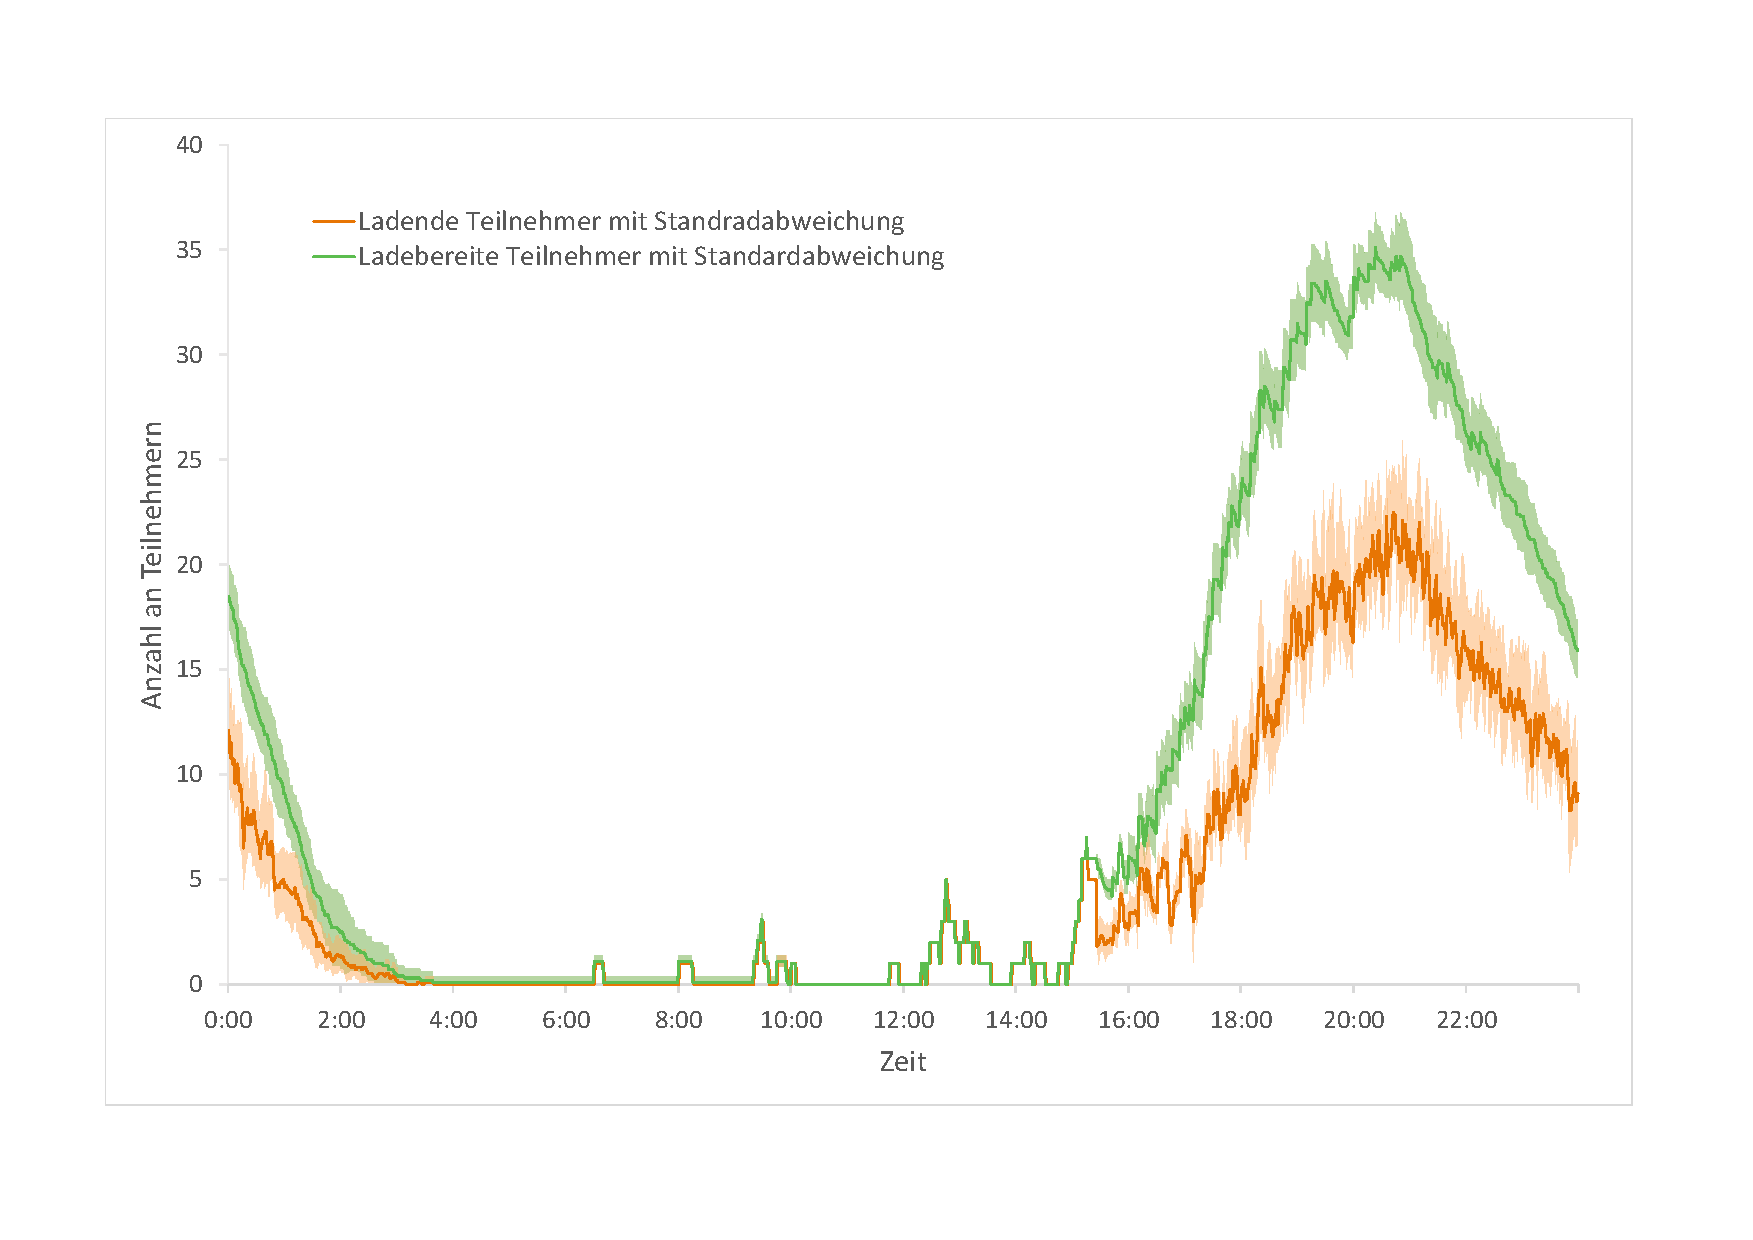
\includegraphics[scale=0.45]{img/SA_wT_trafo/Teilnehmer2.pdf}
	\caption{Teilnehmerzahlen bei Verwendung von SA+T+F+Tr über den Verlauf eines Tages}
	\label{Abb_SAwtTrafo_Teilnehmer}
\end{figure}

Abbildung \ref{Abb_SAparTrafo_Teilnehmer} zeigt die mittlere Anzahl der ladebereiten und tatsächlich ladenden Teilnehmer am Niederspannungsnetz mit den zugehörigen Standardabweichungen. Der Unterschied zwischen den beiden Kurven kommt durch die Vergabe von Wartezeiten zustande, in denen nicht geladen werden kann. Die beiden Kurven haben dieselbe grundlegende Form, während des Verlauf, der beiden Kurven, schwanken die Kurven nur in kleinen Intervallen um die Form der Kurve herum. Je kleiner die Standardabweichung der einzelnen Kurven wird, desto näherer kommen sich die beiden Kurven, allerdings werden dabei auch die Werte an sich geringer. Dadurch lässt sich nur schließen, dass die Ergebnisse der Wartezeitbestimmung starken Einfluss auf das Aussehen dieser Kurven haben.\\
Wie bereits bei der andern Methodik mit dem Transformatorkontroller befinden sich zu Beginn des Tages noch Teilnehmer in Ladeservices, diese werden allerdings zügig abgeschlossen und ab etwa 03:00 habe all diese Teilnehmer ihre Ladeservices abgeschlossen. In dem Zeitraum von etwa 03:00 bis etwa 15:00 treten weder Spannungswerte noch Transformatorwerte, welche in dem jeweiligen Regelbereich liegen, folglich wird in diesem Zeitraum keiner der beiden Kontroller aktiv. Nach 15:00 beginnt die Anzahl der ladebereiten Teilnehmer zu steigen, so steigt auch die Anzahl der ladenden Teilnehmer mit an, wodurch die Transformatorlast steigt und die Spannungswerte zu sinken beginnen. Die Transformatorlast steigt mit der wachsenden Anzahl an ladenden Teilnehmern zunächst immer weiter an, wird allerdings durch den Transformatorkontroller begrenzt und dadurch steigt auch die Anzahl an ladenden Fahrzeug nur bis zu einem gewissen Punkt. An allen drei Graphen ist der Punkt der stärksten Auslastung erkennbar, ab etwa 21:00 beginnen sich die Werte wieder zu bessern. An der Höhe der Kurven ist allerdings erkennbar, dass Ladeservices über das Ende des betrachteten Tages hinaus noch andauern. Zu diesem Zeitpunkt befinden sich allerdings weder Transformatorlast noch Spannung noch Im jeweiligen Regelbereich.\\
Auch die Ergebnisse dieser Methodik wurden gemäß der Einhaltung der Norm DIN EN 50160 betrachtet. Es wurden über alle absolvierten Durchläufe hinweg keinerlei Unterschreitungen der Grenzwerte festgestellt, der Grenzwert von -10~\% p.u. wurde zu keinem Zeitpunkt verletzt, somit wurde auch der Grenzwert bei -15~\% p.u. nicht verletzt. Da keinerlei Verletzungen der Grenzwerte Festgestellt wurden, wurde die Norm erfüllt.\\
Bei der hier betrachteten Methodik wird sowohl auf Spannungskollisionen und auch auf Transformatorkollisionen reagiert. Im Schnitt traten 573,8 ($\pm$ 15,5~\%) Situation ein, wo ein zu niedrige Spannung gemessen wurde und durchschnittlich 7076,1 ($\pm$ 4,3~\%) Situationen, wo eine zu hohe Transformatorlast gemessen wurde. Da beide Arten dieser Situation zeitgleich auftreten können, kam es im Schnitt zu 7077 ($\pm$ 4,3~\%)Situationen in denen eine Kollision auftreten könnte. Tatsächlich ist jedoch nur in durchschnittlich 2482,3 ($\pm$ 2,5~\%) eine Kollision aufgetreten und eine Wartezeit wurde berechnet. Bei 1108800 betrachteten Situation traten im Schnitt lediglich 2482,5 Kollisionen auf, was einem Anteil von 0,22~\% der betrachteten Situationen entspricht. Dir geringe Anzahl an berechneten Wartezeiten bedeutet, das die berechneten Wartezeiten effektiv bestimmt wurden und ihren angedachten Zweck, nämlich weitere Kollisionen zu verhindern, erfüllt haben.\\
Alle im Simulationszeitraum von einer Woche gestarteten Ladeservice wurden erfolgreich abgeschlossen, somit ist die Qualität der Ladeservice maximal. Abbildung \ref{ABB_SAwtTrafo_SocMEAN} zeigt den mittleren Ladestand aller Fahrzeuge über Verlauf der jeweiligen Ladeservice hinweg, Abbildung \ref{ABB_SAwtTrafo_SocSTD} zeigt die dazugehörige Standardabweichung.\\
\begin{figure}
	\begin{subfigure}{0.49\linewidth}
		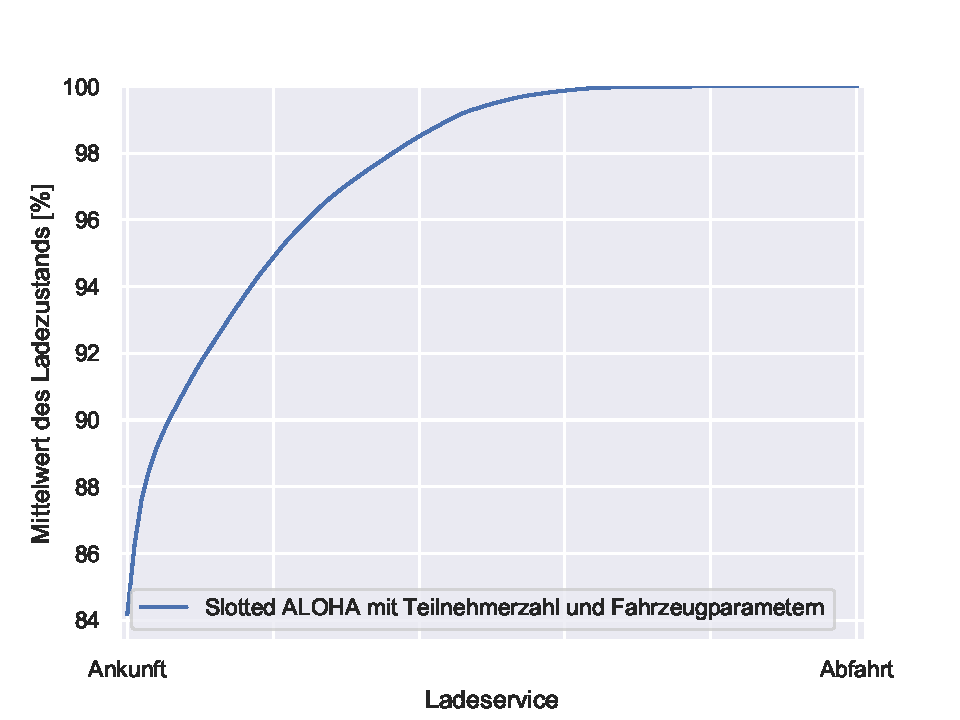
\includegraphics[width=\linewidth]{img/SA_wt_trafo/SlottedAloha_waitingTime_VDE_tau_trafo_13_soc_mean.pdf}
        \subcaption{Durchschnittlicher Ladezustand aller Elektrofahrzeuges über den Verlauf eines Ladeservices}
        \label{ABB_SAwtTrafo_SocMEAN}
	\end{subfigure}
	\begin{subfigure}{0.49\linewidth}
		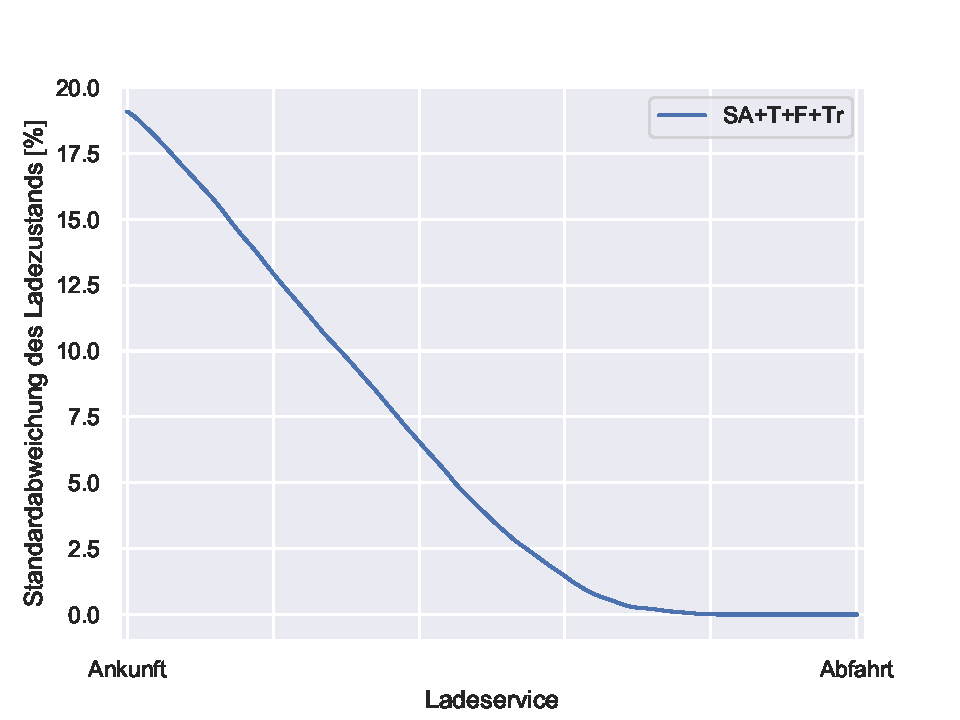
\includegraphics[width=\linewidth]{img/SA_wT_trafo/SlottedAloha_waitingTime_VDE_tau_trafo_13_soc_std.pdf}
        \subcaption{Durschschnittliche Standardabweichung des Ladezustandes aller Elektrofahrzeuges über den Verlauf eines Ladeservices}
        \label{ABB_SAwtTrafo_SocSTD}
	\end{subfigure}
	\caption{Durchschnittlicher Ladezustand mit Standardabweichung bei Verwendung von SA+T+F+Tr}
\end{figure}
Den beiden Abbildungen ist zu entnehmen, dass in Schnitt nach 70 \% der Zeit eines Ladeservices der Ladeservice als erfolgreich eingestuft werden kann, da der Ladestand auf 100 \% angestiegen ist und die Standardabweichung des Ladestandes auf 0 \% gefallen ist. Die Standardabweichung sinkt langsamer als der Ladestand steigt, was darauf hindeutet, dass durch die besser gewählten Wartezeiten, die Fahrzeuge besser zeitlich verteilt werden, wodurch die Unterschiede im Ladestand länger bestehen bleiben.\\
\begin{figure}[htb]
\centering
	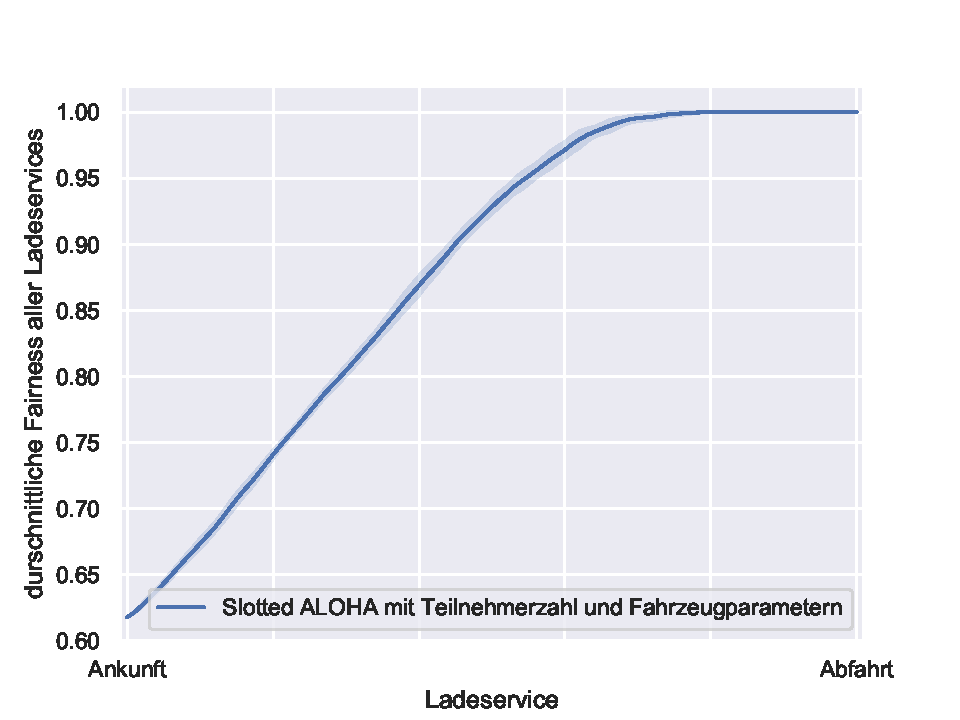
\includegraphics[scale=0.45]{img/Sa_wT_trafo/SlottedAloha_waitingTime_VDE_tau_trafo_13_qoe.pdf}
	\caption{Durchschnittlicher Qualitätserfahrung Fairness Index aller Elektrofahrzeuges über den Verlauf eines Ladeservices bei Verwendung der Methodik SA+T+F+Tr}
	\label{Abb_SAwtTrafo_Fairness}
\end{figure}
Abbildung \ref{Abb_SAwtTrafo_Fairness} zeigt den gemittelten Fairness Index aller Teilnehmer über den zeitlichen Verlauf der Ladeservice hinweg mit der zugehörigen Standardabweichung. Die geringe Standardabweichung weist auf ähnliche Werte, über alle Durchläufe hinweg, hin. Die Fairness steigt an wie die Standardabweichung des Ladestandes fällt. Der Fairness Index steigt beständig an, bis der Wert bei nach etwa 75 \% der Zeit der Ladeservices maximal wird und auf diesem Niveau bleibt. Die Fairness steigt hier langsamer als bei anderen Methoden, erreicht jedoch trotzdem den maximal möglichen Wert.

\section{Analyse und Auswertung}
Nachdem alle Varianten nun jeweils einzeln analysiert wurden, folgt nun ein Vergleich über jeweils drei der Varianten, gruppiert nach der Verwendung des Transformatorkontrollers. Betrachtet werden die selben Messwerte wie bereits bei den Einzelanalysen und auch bei diesen Analysen wird bei der Transformatorlast, den Spannungswerten und den Teilnehmerzahlen jeweils nur ein Werktag dargestellt.
\subsection{Vergleich der Varianten ohne Transformatorkontroller}
Es werden nun die drei Methodiken miteinander verglichen, welche keinen Transformatorkontroller verwenden. Diese drei Techniken wurden in den Kapiteln \ref{chap_VDE}, \ref{chap_SApar}, \ref{chap_SAwt} jeweils einzeln für sich analysiert, nun folgt ein Vergleich und eine Analyse über alle drei Varianten hinweg.
\begin{figure}
	\begin{subfigure}{\linewidth}
		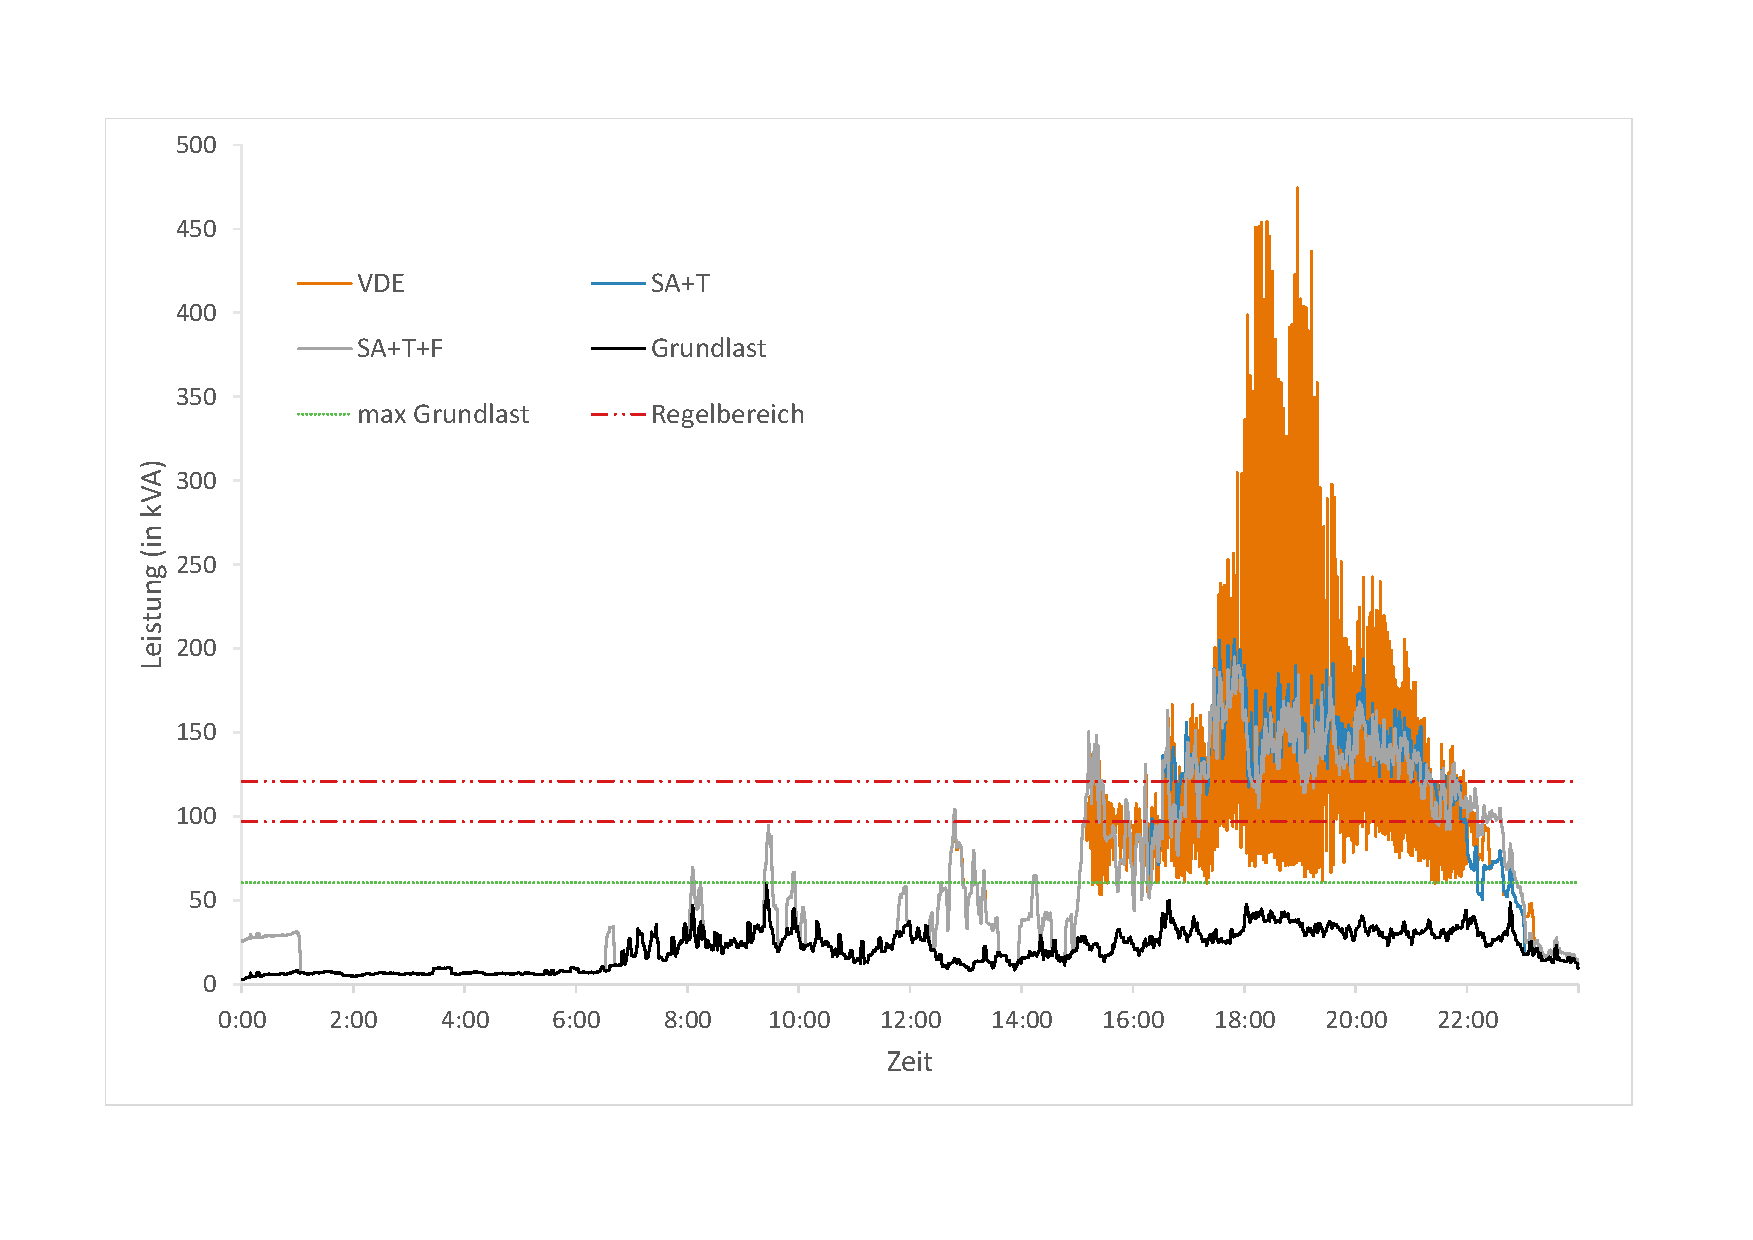
\includegraphics[scale=0.45]{img/ohneTrafo/TrafoLast6.pdf}
		\caption{Transformatorlast über den Verlauf eines Tages}
		\label{Abb_oT_TrafoLast}
	\end{subfigure}
	\begin{subfigure}{\linewidth}
		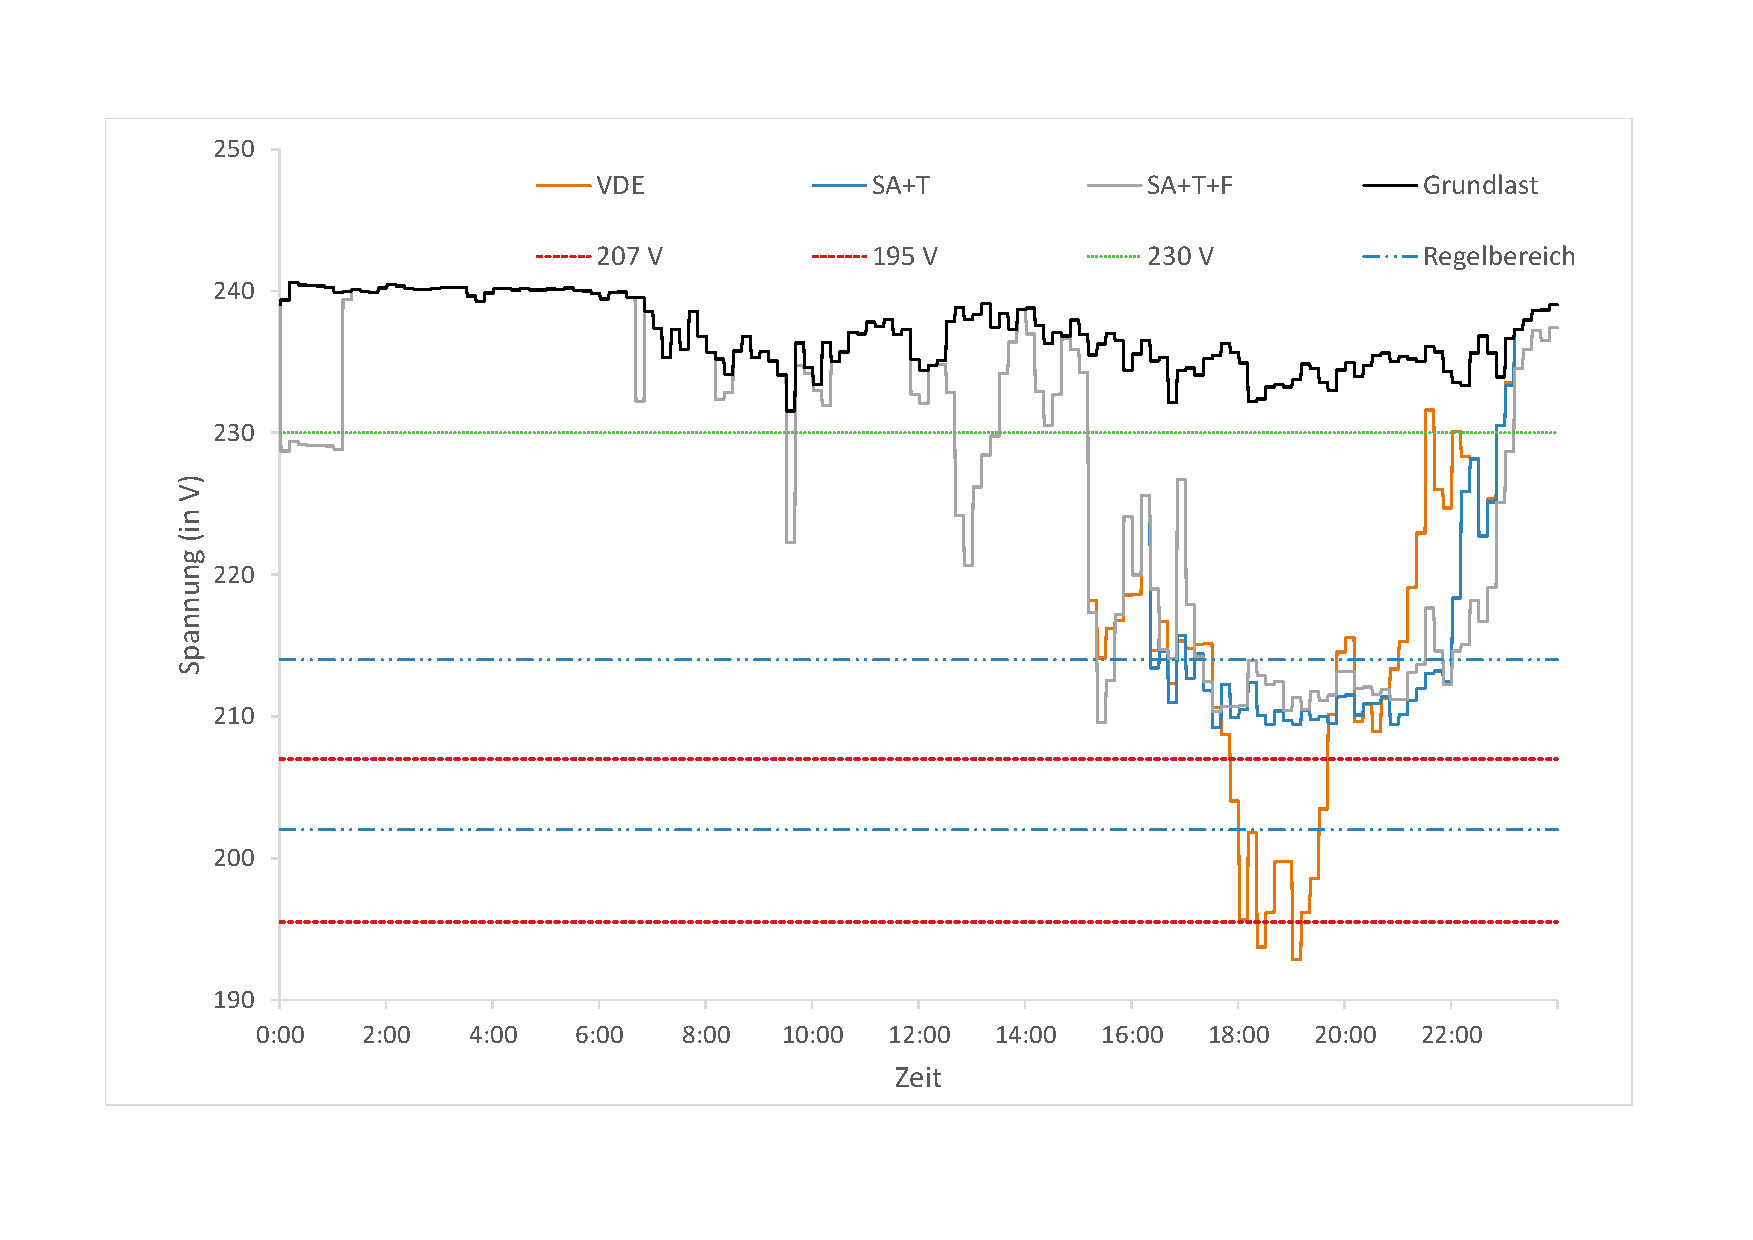
\includegraphics[scale=0.45]{img/ohneTrafo/Spannung5.pdf}
		\caption{10 Minuten Mittelwerte der Spannung über den Verlauf eines Tages}
		\label{Abb_oT_Spannung}
	\end{subfigure}
	\caption{Transformatorlast und Spannungsverlauf bei Verwendung von VDE, SA+T+F und SA+T+F}
\end{figure}
In Abbildung \ref{Abb_oT_TrafoLast} wird der Leistungsbezug am Transformator, welcher von jeder der drei Methodiken verursacht wurde, abgebildet. Der Regelbereich ist hier zwar angetragen, jedoch verfügt keine der hier dargestellten Techniken über den entsprechenden Kontroller. Anders als bei den Einzelanalysen wird hier auf das abbilden der Standardabweichung verzichtet, um eine bessere Übersichtlichkeit zu erhalten. An den Graphen wird der Effekt der Verwendung des Slotted Aloha Protokolls deutlich. Die Transformatorlast, wenn nur der VDE-Kontroller verwendet wird, schwankt stärker und erreicht höhere Werte als die beiden Varianten, welche das Slotted Aloha Protokoll verwenden. Die beiden Varianten, welche das Protokoll verwenden, weisen ähnliche Werte auf, beider Arten der Bestimmung der Wartezeiten zeigen hier, dass das Konzept funktioniert und zu einer Besserung der Werte beitragen kann. Diese Besserung stellt ein unabhängig von der Art der Bestimmung der Wartezeit. Das spätere Sinken der Last, bei SA+T+F, zeigt diese die Ladevorgänge bei dieser Variante auf längere Zeit verteilt wurden, dies ist auch an dem gelegentlich niedrigeren Werten bereits ablesbar.\\
Abbildung \ref{Abb_oT_Spannung} zeigt die minimalen 10 Minuten Mittelwerte aller Anschlusspunkte des Niederspannungsnetzes. Der angetragene Regelbereich kennzeichnet den Bereich, in dem der Spannungskontroller aktiv wird und den möglichen Lastbezug regelt. Auch in dieser Abbildung werden die jeweiligen Standardabweichungen zur besseren Übersichtlichkeit nicht dargestellt. Im Vergleich über die drei hier dargestellten Methodiken zeigt sich, wie bereits bei der Transformatorlast, dass der VDE-Kontroller ohne Slotted Aloha nicht in der Lage ist die Werte ausreichend zu kontrollieren. Die beiden Methodiken, welche das Slotted Aloha Protokoll mitverwenden, zeigen anhand ihrer Graphen, wie der Spannungskontroller seinen angedachten Zweck erfüllt. Die Werte fallen zwar auch in den Regelbereich ab, bleiben allerdings oberhalb der unteren Grenze des Regelbereiches. Der Verlauf der beiden Graphen, währenddessen sie im Regelbereich liegen, zeigt einen ähnlichen Verlauf ohne zu große Schwankungen. Auch bei der Spannung erholen sich die Werte, bei der Variante, welche nur die Teilnehmeranzahl verwendet, schneller als bei der anderen Variante, welche das Slotted Aloha Protokoll mitverwendet. Allerdings ist am Verlauf des Graphen auch erkennbar, dass die Werte bei SA+T+F im Regelbereich des Kontrollers noch am höchsten sind und nur die Rückkehr zur Grundlast etwas länger dauert.
\begin{figure}
	\begin{subfigure}{\linewidth}
		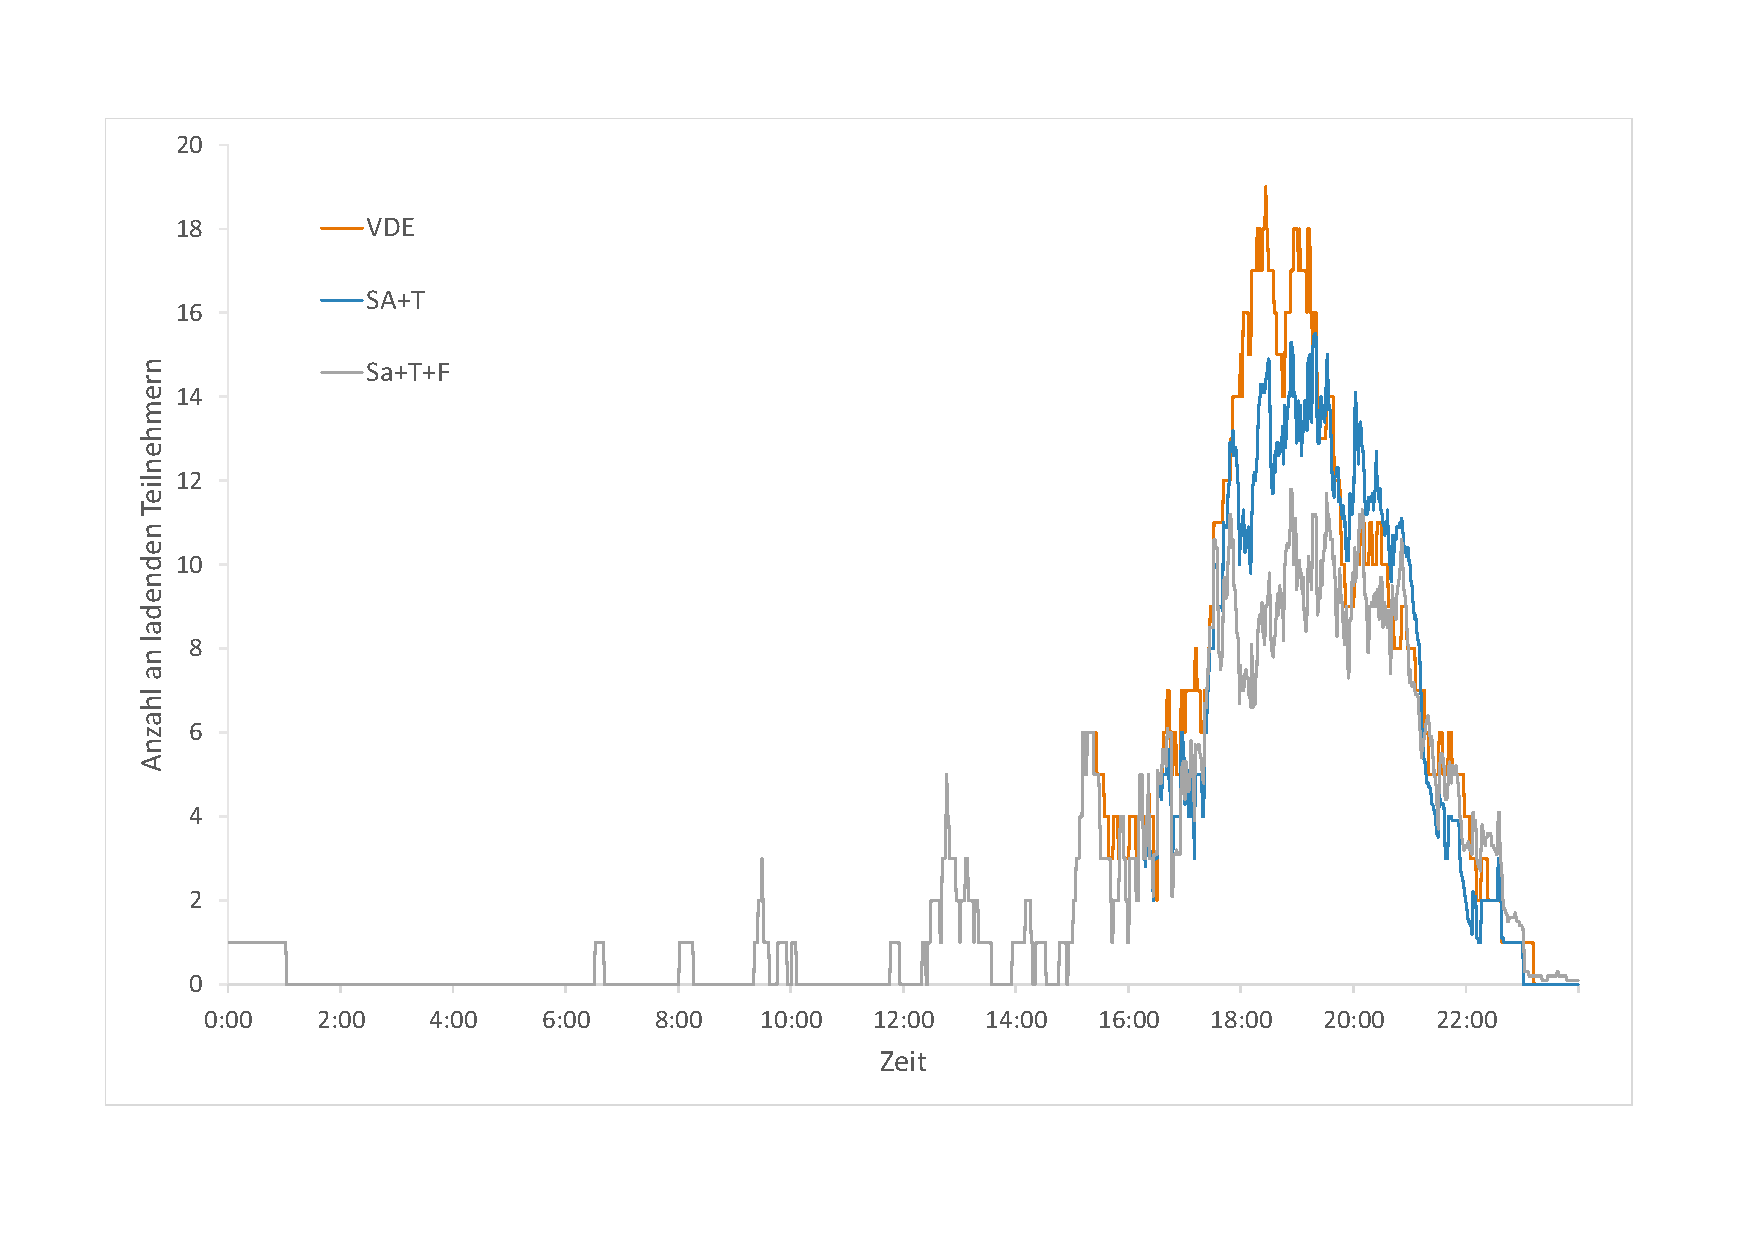
\includegraphics[scale=0.45]{img/ohneTrafo/Teilnehmer_laden.pdf}
        \subcaption{Anzahl der ladenden Teilnehmer über den Verlauf eines Tages}
        \label{ABB_oT_Teil1}
	\end{subfigure}
	\begin{subfigure}{\linewidth}
		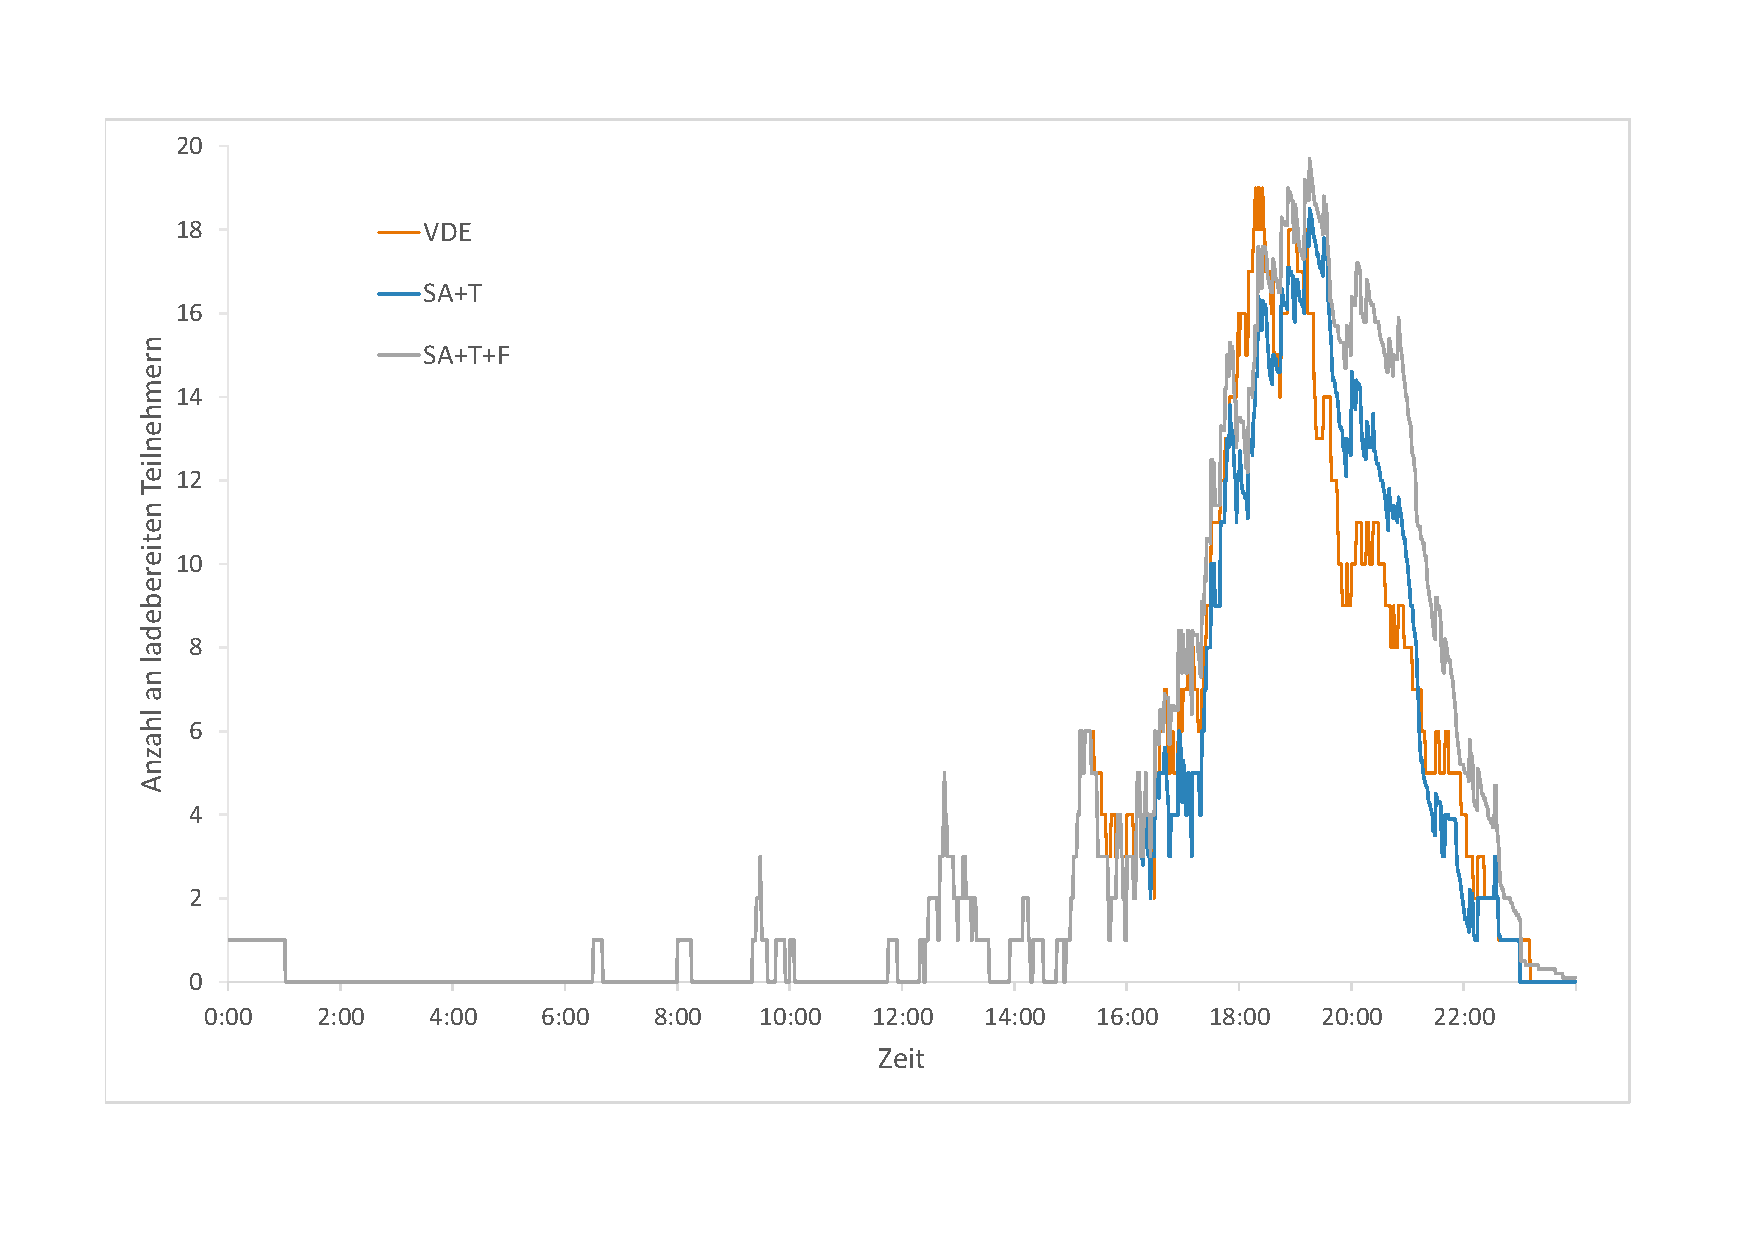
\includegraphics[scale=0.45]{img/ohneTrafo/Teilnehmer_bereit2.pdf}
        \subcaption{Anzahl der ladendbereiten Teilnehmer über den Verlauf eines Tages}
        \label{ABB_oT_teil2}
	\end{subfigure}
	\caption{Teilnehmerzahlen bei Verwendung von VDE, SA+T+F und SA+T+F}
\end{figure}
In Abbildung \ref{ABB_oT_Teil1} sind die jeweiligen Anzahlen der ladenden Teilnehmer und in Abbildung \ref{ABB_oT_teil2} die jeweiligen Anzahlen der ladebereiten Teilnehmer dargestellt. An der Zahl der Teilnehmer ist erkennbar, dass die über alle drei Methoden hinweg die zahl der ladebereiten Teilnehmer immer relativ ähnlich ist, während sich bei der Anzahl der ladenden Teilnehmer teils sichtbare Unterschiede einstellen. Bei der Methode, wo sowohl Teilnehmerzahl als auch Fahrzeugparameter verwendet werden, laden meist weniger Teilnehmer gleichzeitig, dafür gibt es über einen längeren Zeitraum mehr ladebereite Teilnehmer. Bei der Anzahl der ladenden Teilnehmer zeigt sich der Unterschied in der Bestimmung der Ladezeiten, durch die Möglichkeit längere Wartezeit zu bestimmen, da durch die Verwendung der Fahrzeugparameter die Ergebnismenge nicht mehr durch die Anzahl an Ladebereiten Teilnehmern beschränkt ist. Die hier sichtbare unterschiedliche Verteilung der ladenden Teilnehmer zeigte sich bereits bei der Transformatorlast und den Spannungswerten.
Beim Vergleich über die Transformatorlast, den Spannungsverlauf und die Teilnehmerzahlen zeigt sich, dass die beiden Varianten, die das Aloha Protokoll mitverwenden im Vergleich zum VDE-Kontroller bessere Ergebnisse liefern. Die Transformatorlasten sind deutlich kontrollierter und die Spannungswerte liegen höher. Diese Muster setzt sich bei der Betrachtung der Einhaltung der Norm DIN EN 50160 fort, von den drei betrachteten Methoden ist lediglich der VDE-Kontroller nicht in der Lage diese Norm zu erfüllen.
Für alle drei Methoden wurde die Anzahl an Situation bestimmt, in denen eine Spannungskollision auftreten könnte.
\begin{table}[]
\centering
\begin{tabular}{l|l|l|l|}
\cline{2-4}
                                                                                       & Variante &            &            \\ \hline
\multicolumn{1}{|l|}{}                                                                 & VDE      & SA+T       & SA+T+F     \\ \hline
\multicolumn{1}{|l|}{\begin{tabular}[c]{@{}l@{}}mögliche \\ Situationen\end{tabular}}  & 1535.0   & 668.7 ($\pm$ 6.7~\%) & 392.6 ($\pm$ 12.2~\%) \\ \hline
\multicolumn{1}{|l|}{\begin{tabular}[c]{@{}l@{}}Anzahl an \\ Wartezeiten\end{tabular}} & 0.0      & 553.9 ($\pm$ 5.9~\%) & 246.9 ($\pm$ 9.2~\%) \\ \hline
\end{tabular}
\caption{Anzahl der möglichen und tatsächlich aufgetreten Kollisionen bei den Methoden VDE, SA+T und SA+T+F}
\label{tab:my-table3}
\end{table}

Anhand Tabelle \ref{tab:my-table3} zeigt sich erneut die Verbesserung die erzielt wird, wird eine Variante verwendet, welche mit Teilen des Netzwerkprotokolls erweitert wurde. Je nach verwendeter Variante treten nur noch halb bzw. ein Viertel so viele Situationen ein, wo eine Spannungskollision auftreten könnte. Jedoch zeigt sich auch beim Vergleich der beiden Varianten, welche das Protokoll mitverwenden, wie sich die Arten der Wartezeitbestimmung unterscheiden, da auch hier, wenn Teilnehmerzahl und Fahrzeugparameter verwendet werden, die Anzahl an Situationen um mehr als ein Drittel reduziert werden kann. Mit der Anzahl der möglichen Kollisionen sinkt auch die Zahl der aufgetretenen Kollisionen. Beim Verhältnis zwischen möglichen und tatsächlich aufgetretenen Kollisionen, zeigt sich, dass wenn die Fahrzeugparameter mitberücksichtigt werden, in weniger Situationen wo eine Kollision auftreten kann auch eine Kollision auftritt. Wird nur die Teilnehmerzahl verwendet wird in etwa 80~\% der möglichen Situationen auch eine Wartezeit bestimmt, werden nun zusätzlich die Fahrzeugparameter berücksichtigt sinkt dieser Wert auf etwa 60~\% ab. 
\begin{figure}
	\begin{subfigure}{0.49\linewidth}
		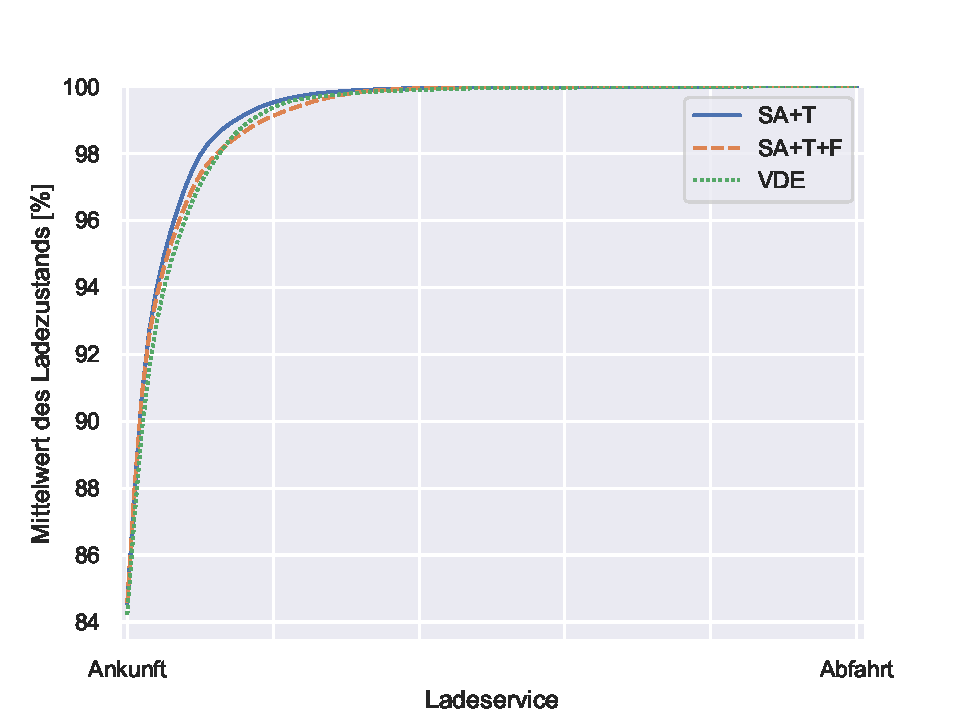
\includegraphics[width=\linewidth]{img/ohneTrafo/SlottedAloha_participants_VDE_tau_13_soc_mean.pdf}
        \subcaption{Durchschnittlicher Ladezustand aller Elektrofahrzeuges über den Verlauf eines Ladeservices}
        \label{ABB_ot_SocMEAN}
	\end{subfigure}
	\begin{subfigure}{0.49\linewidth}
		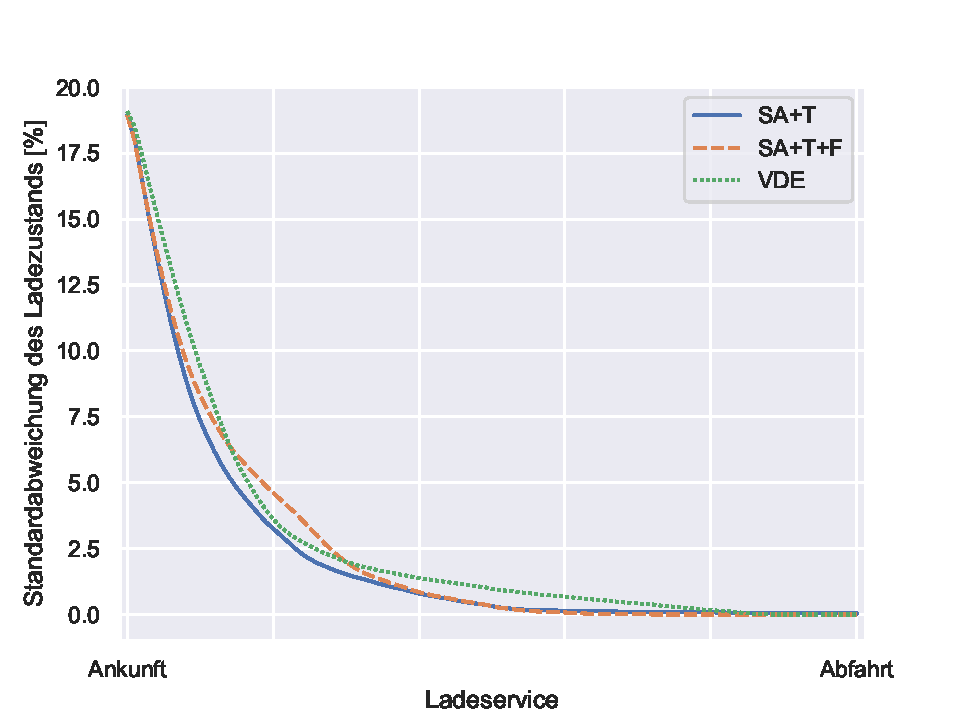
\includegraphics[width=\linewidth]{img/ohneTrafo/SlottedAloha_participants_VDE_tau_13_soc_std.pdf}
        \subcaption{Durschschnittliche Standardabweichung des Ladezustandes aller Elektrofahrzeuges über den Verlauf eines Ladeservices}
        \label{ABB_oT_SocSTD}
	\end{subfigure}
	\caption{Durchschnittlicher Ladezustand mit Standardabweichung bei Verwendung von VDE, SA+T+F und SA+T+F}
\end{figure}

In Abbildung \ref{ABB_ot_SocMEAN} sind die jeweiligen mittleren Ladestände aller Fahrzeugen über den Verlauf der Ladeservice hinweg dargestellt, Abbildung \ref{ABB_oT_SocSTD} zeigt die zugehörige Standardabweichung. Abbildung \ref{ABB_ot_SocMEAN} zeigt einen ähnlichen Verlauf der Kurven für alle drei Varianten, wird allerdings zusätzlich die dazugehörige Standardabweichung betrachtet zeigen sich Unterschiede. Diese Unterschiede weisen erneut auf das bekannte Verhältnis zwischen den Varianten hin. Sichtbar wird auch die Ähnlichkeit der beiden Varianten, welche Wartezeiten verwenden.
\begin{figure}[htb]
\centering
	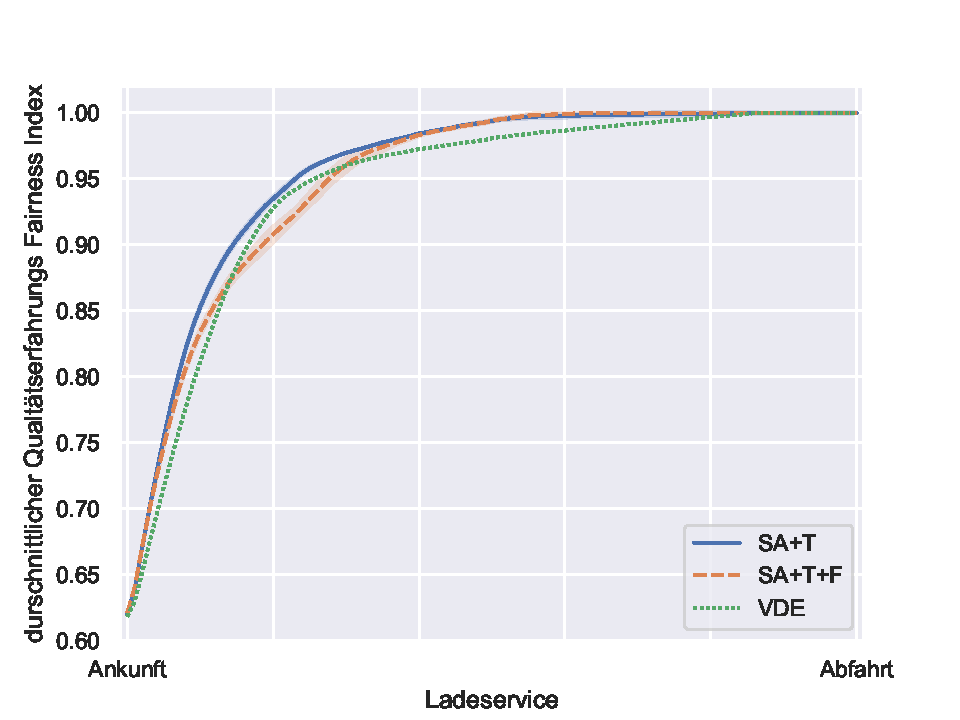
\includegraphics[scale=0.45]{img/ohneTrafo/SlottedAloha_participants_VDE_tau_13_qoe.pdf}
	\caption{Durchschnittlicher Qualitätserfahrungs Fairness Index aller Elektrofahrzeuges über den Verlauf eines Ladeservices bei Verwendung von VDE, SA+T+F und SA+T+F}
	\label{Abb_oT_Fairness}
\end{figure}
Abbildung \ref{Abb_oT_Fairness} zeigt die mittlere Fairness aller Fahrzeuge über den Verlauf der Ladeservice hinweg mit der zugehörigen Standardabweichung für alle drei betrachteten Varianten. Der Verlauf der drei Kurven weist auch hier wieder große Ähnlichkeiten auf. Allerdings erreichen die beiden Varianten, welche Teile des Aloha Netzwerkprotokolls verwenden, den maximalen Wert deutlich früher als der VDE-Kontroller. Die beiden Varianten mit dem Netzwerkprotokoll erreichen den maximal Wert nahezu gleichzeitig, im Verlauf der Graphen zeigen sich dennoch Unterschiede. Der teils langsamere Anstieg kann auf die bessere Verteilung der Ladevorgänge über die Zeit zurückgeführt werden. Diese bessere Verteilung hat sich bei der Betrachtung bisher als positive Eigenschaft herausgestellt und mindert auch hier das eigentlich erreichte Ergebnis nicht.
Nach Betrachtung der Eigenschaften über alle drei Varianten hat sich herausgestellt, dass die Varianten, welche teile des Aloha Protokolls verwenden, bessere Ergebnisse geliefert haben als der VDE-Kontroller ohne Erweiterung. Aus dem Vergleich ging des Weiteren hervor, dass die Variante, welche die Teilnehmerzahl und die Fahrzeugparameter verwendet, das beste der drei Ergebnisse liefert. Diese Variante sorgt für höhere Spannungen, niedrige Transformatorlasten, es kommen am wenigsten Situationen vor, in denen eine Spannungskollision auftreten könnte und all das wird erreicht während zudem der Zeitpunkt, an dem maximal mögliche Fairness zwischen den Teilnehmern erreicht wird, nach vorne verlegt wird.

\subsection{Vergleich der Varianten mit Transformatorkontroller}
Die Ergebnisse der drei Varianten, welche den Transformatorkontroller verwenden, wurden bereits jeweils für sich analysiert, nun folgt der Vergleich über die drei Varianten hinweg. Wie bereits bei der Analyse des VDE-Kontrollers mit dem Transformatorkontroller erwähnt wurde, musste bei dieser Variante der verwendete Lag-Filter geändert werden, um einen erfolgreichen und vollständigen Durchlauf zu erhaltenen. Diese Änderung beeinflusst auch das Ergebnis dieses Vergleichs, da sie nur bei einer Methodik notwendig war und die anderen beiden Varianten, einen anderen Lag-Filter verwenden.\\
\begin{figure}
	\begin{subfigure}{\linewidth}
		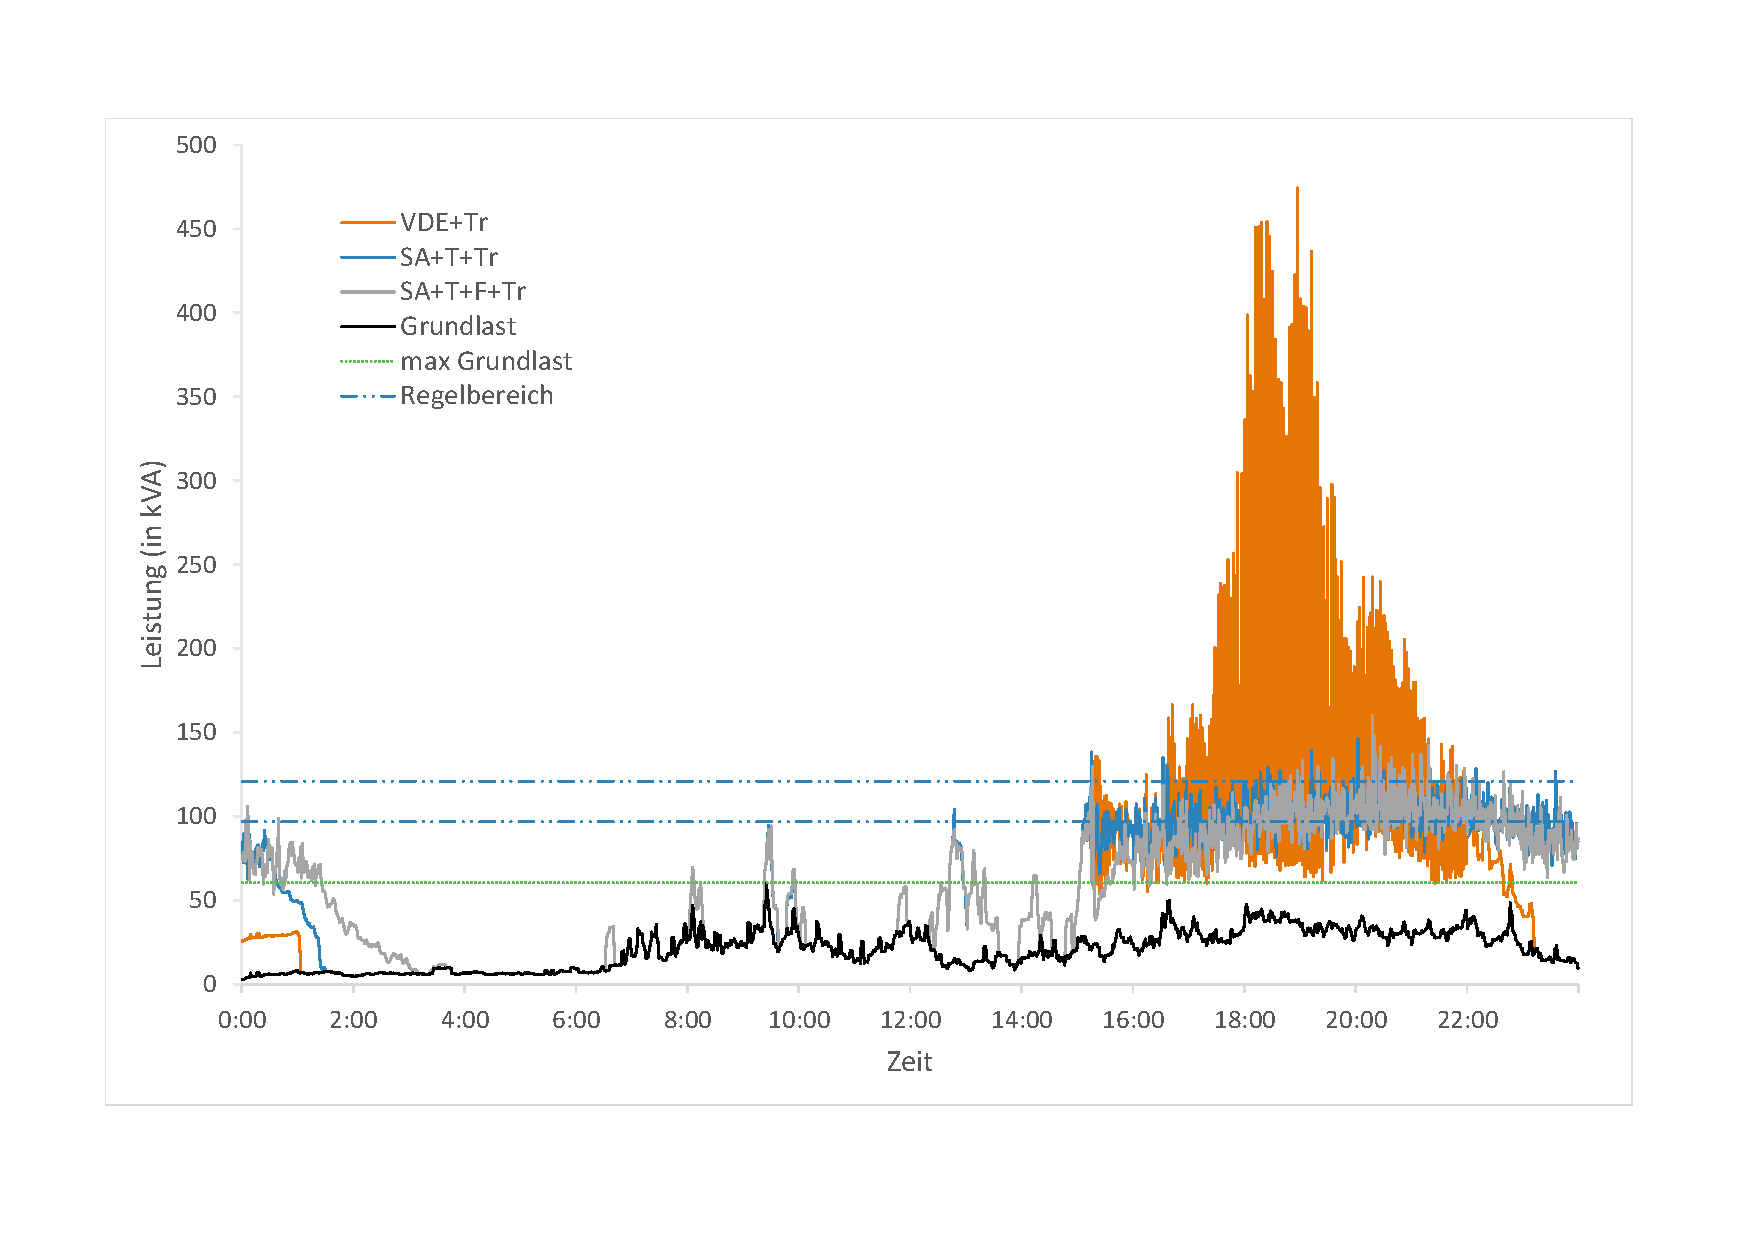
\includegraphics[scale=0.45]{img/mitTrafo/Trafolast2.pdf}
        \subcaption{Transformatorlast über den Verlauf eines Tages}
        \label{ABB_mT_Trafo}
	\end{subfigure}
	\begin{subfigure}{\linewidth}
		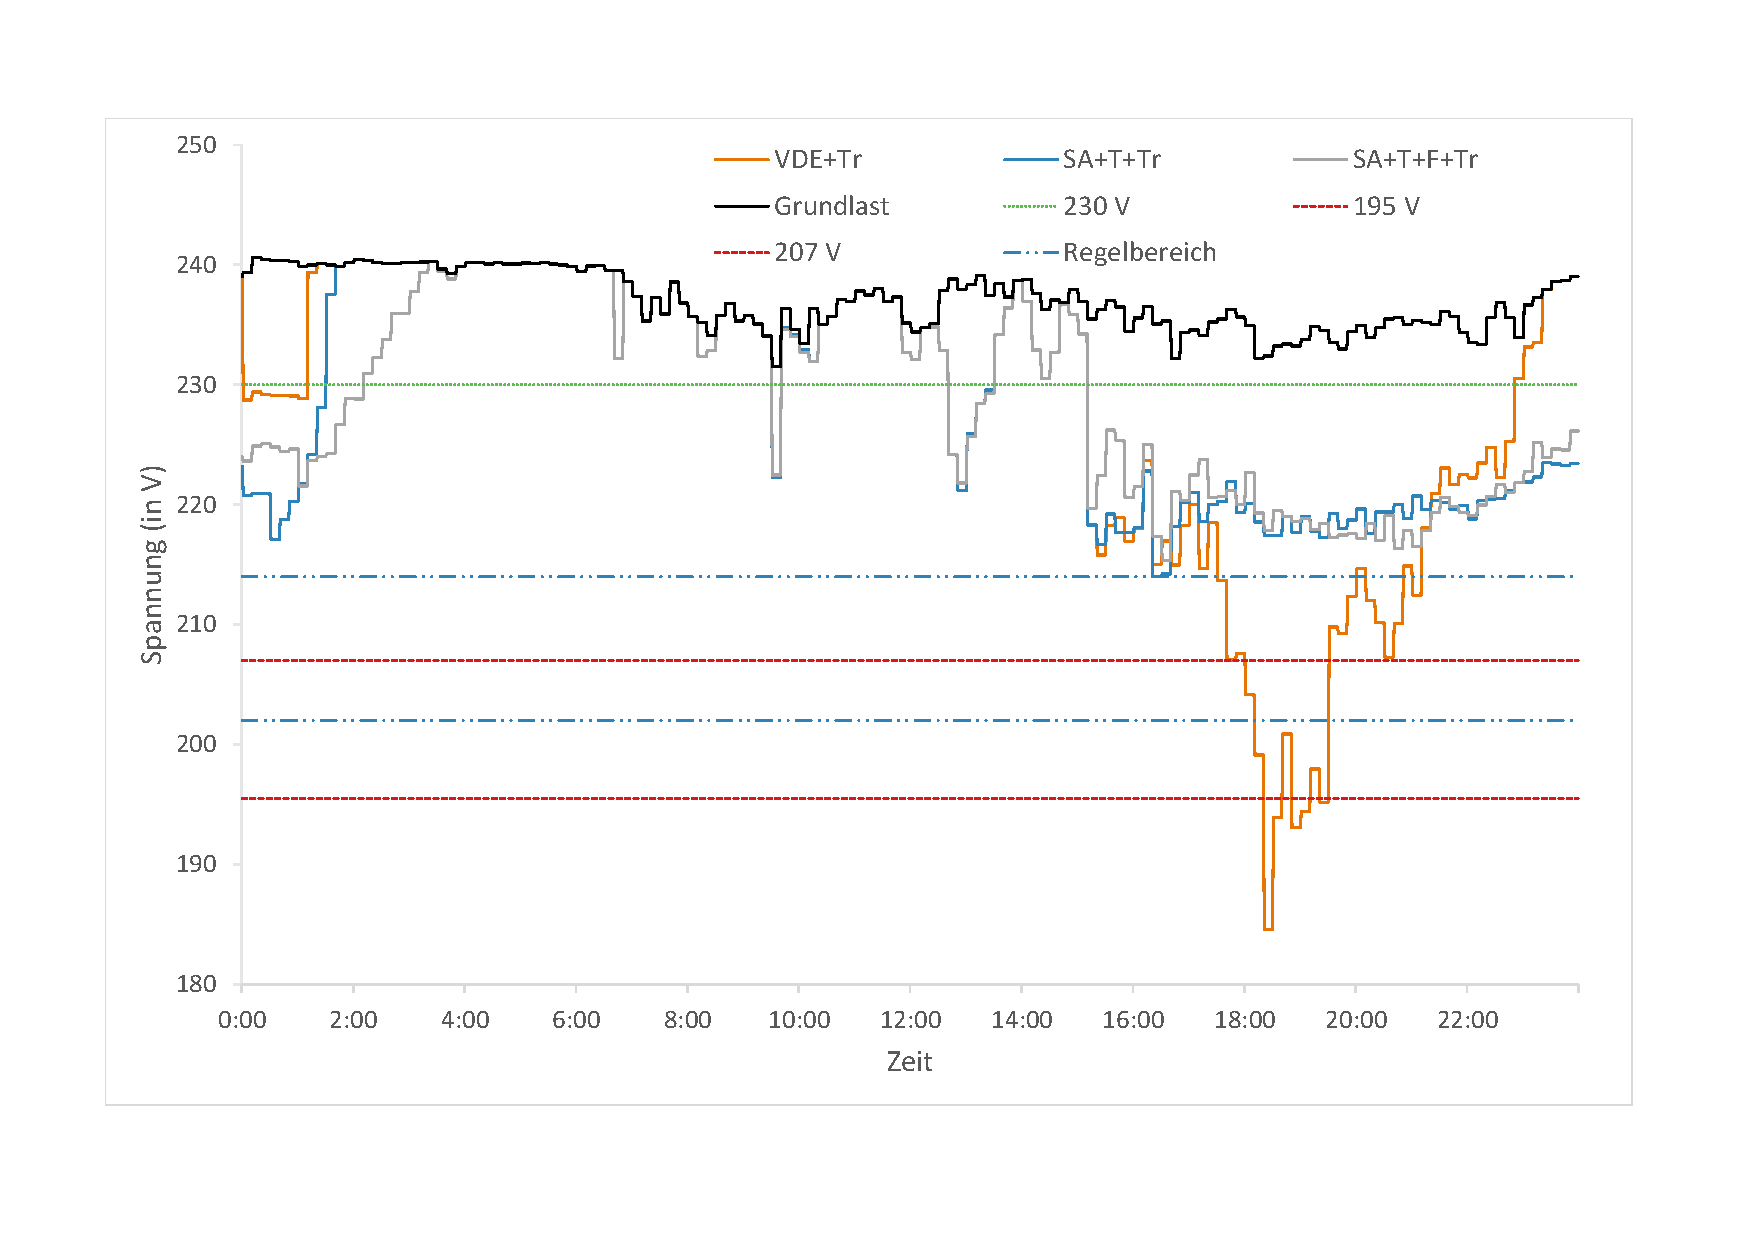
\includegraphics[scale=0.45]{img/mitTrafo/Spannung2.pdf}
        \subcaption{10 Minuten Mittelwerte der Spannung über den Verlauf eines Tages}
        \label{ABB_mT_Spannung}
	\end{subfigure}
	\caption{Transformatorlast und Spannungsverlauf bei Verwendung von VDE+Tr, SA+T+Tr und SA+T+F+Tr}
\end{figure}
In Abbildung \ref{ABB_mT_Trafo} sind die mittleren Transformatorlasten der drei verwendeten Methoden angetragen. Der nach unten und oben abgegrenzte Regelbereich markiert den Arbeitsbereich des Transformatorkontrollers. Einzelne Spitzen über den Regelbereich hinaus, lassen sich aufgrund der dezentralen Verwendung kaum verhindern, da sich die einzelnen Teilnehmer nicht mit anderen abstimmen. Am Verlauf der Kurven erkennt man dasselbe Muster, welche sich bereits bei der Analyse aller drei Varianten ohne Transformatorkontroller gezeigt hat. Die Variante mit nur dem VDE-Kontroller oszilliert sehr stark und liefert die höchsten Werte aller drei Varianten. Die beiden Varianten, welche mit Teilen des Aloha Netzwerkprotokolls erweitert wurden, liefern sehr ähnliche Werte. Jedoch zeigt sich erneut, dass wenn die Fahrzeugparameter mit berücksichtigt werden, die Last zwar länger braucht um wieder auf das Niveau der Grundlast abzusinken, allerdings sind die Werte auch etwas niedriger als, wenn nur die Teilnehmerzahl verwendet wird.\\
Abbildung \ref{ABB_mT_Spannung} zeigt die Mittelwerte von 10 Minuten Mittelwerten der Spannung, auf die Abbildung der dazugehörigen Standardabweichung wurde für eine bessere Übersichtlichkeit verzichtet. Hier wiederholt sich erneut das bereits festgestellte Muster. Der VDE-Kontroller ohne Erweiterungen liefert das schlechteste Ergebnis, während sich die Ergebnisse der beiden erweiterten Varianten sehr ähnlich sind. Ein merklicher Unterschied zwischen den beiden erweiterten Varianten lässt sich hier nur zum Beginn des betrachteten Zeitraumes feststellen, wo die Variante, welche die Teilnehmerzahl und die Fahrzeugparameter verwendet, zunächst höhere Werte aufweist, die Rückkehr auf das Niveau der Grundlast allerdings länger dauert.\\
\begin{figure}
	\begin{subfigure}{\linewidth}
		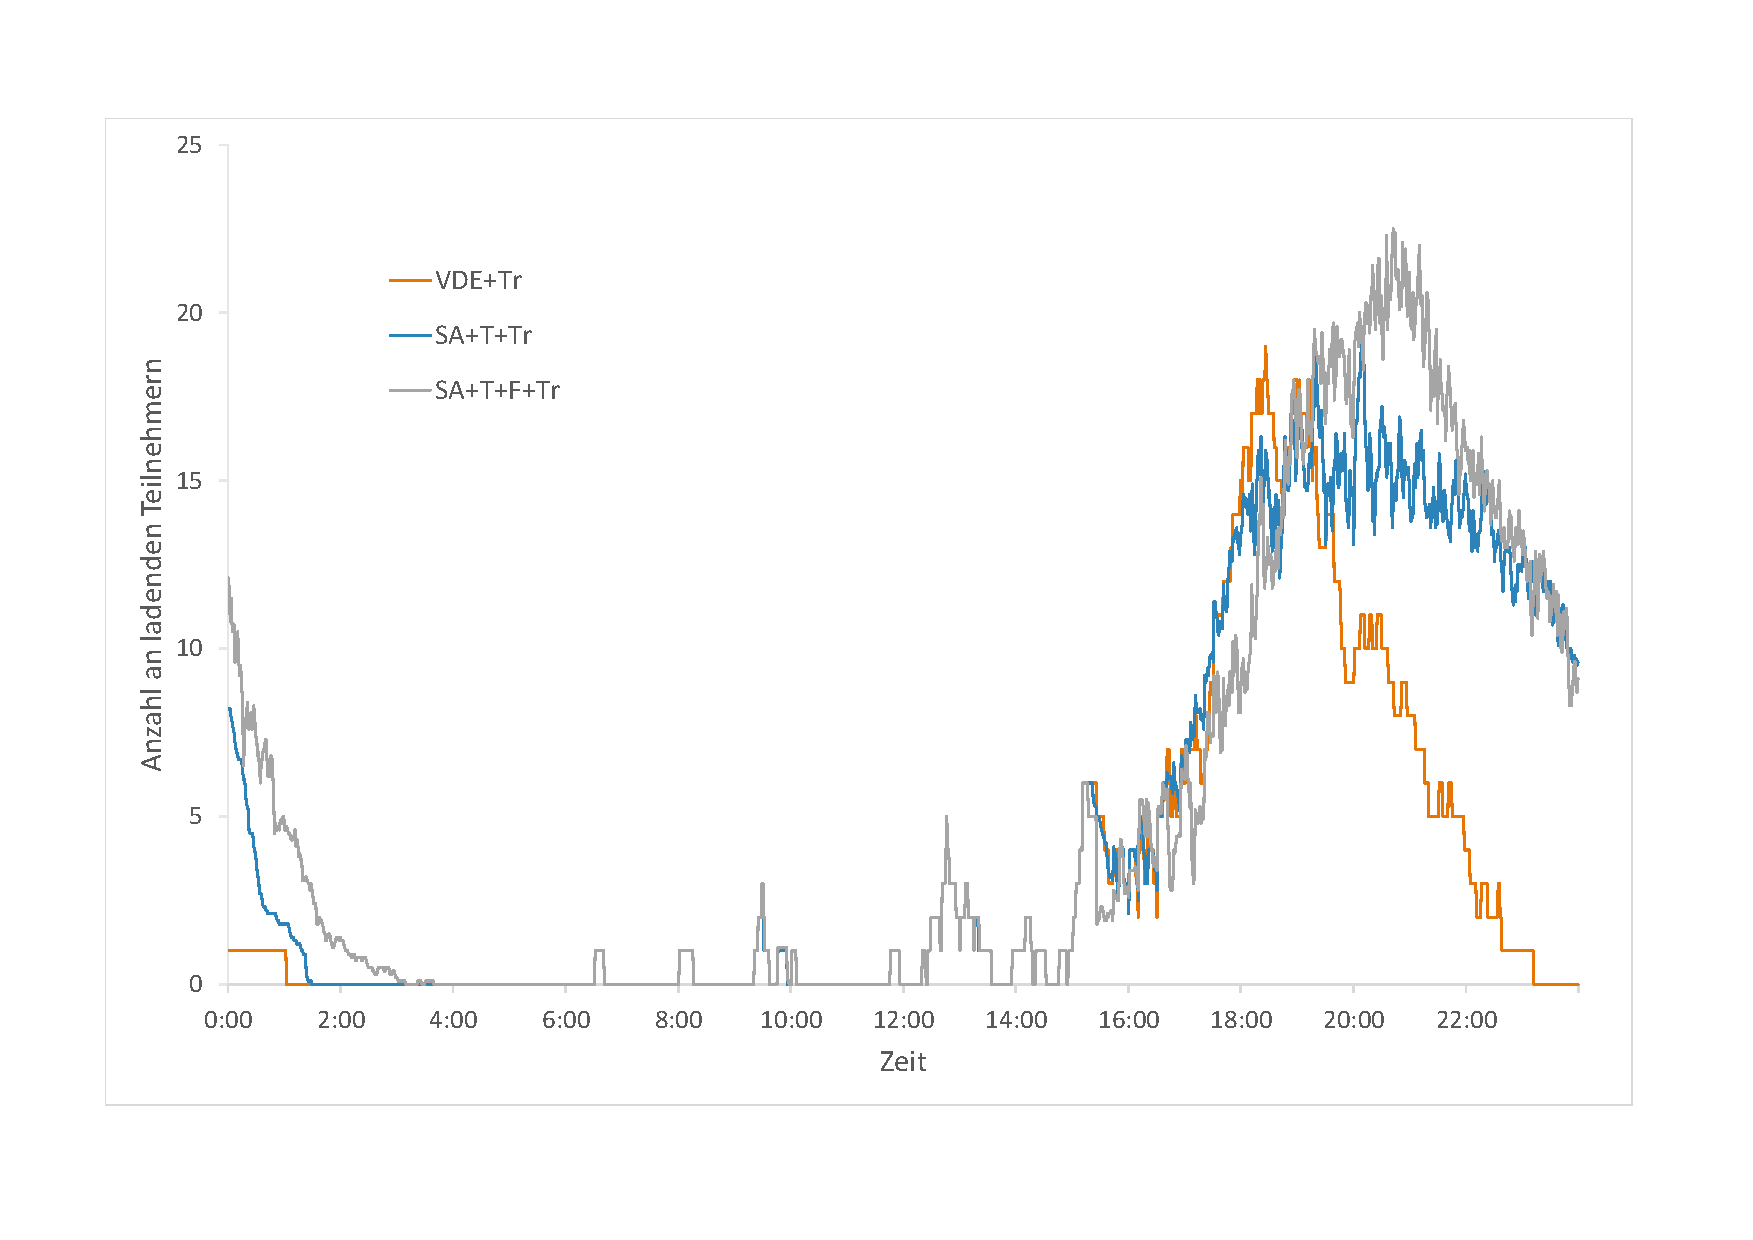
\includegraphics[scale=0.45]{img/mitTrafo/Teilnehmer_laden.pdf}
        \subcaption{Anzahl der ladenden Teilnehmer über den Verlauf eines Tages}
        \label{ABB_mT_Teil1}
	\end{subfigure}
	\begin{subfigure}{\linewidth}
		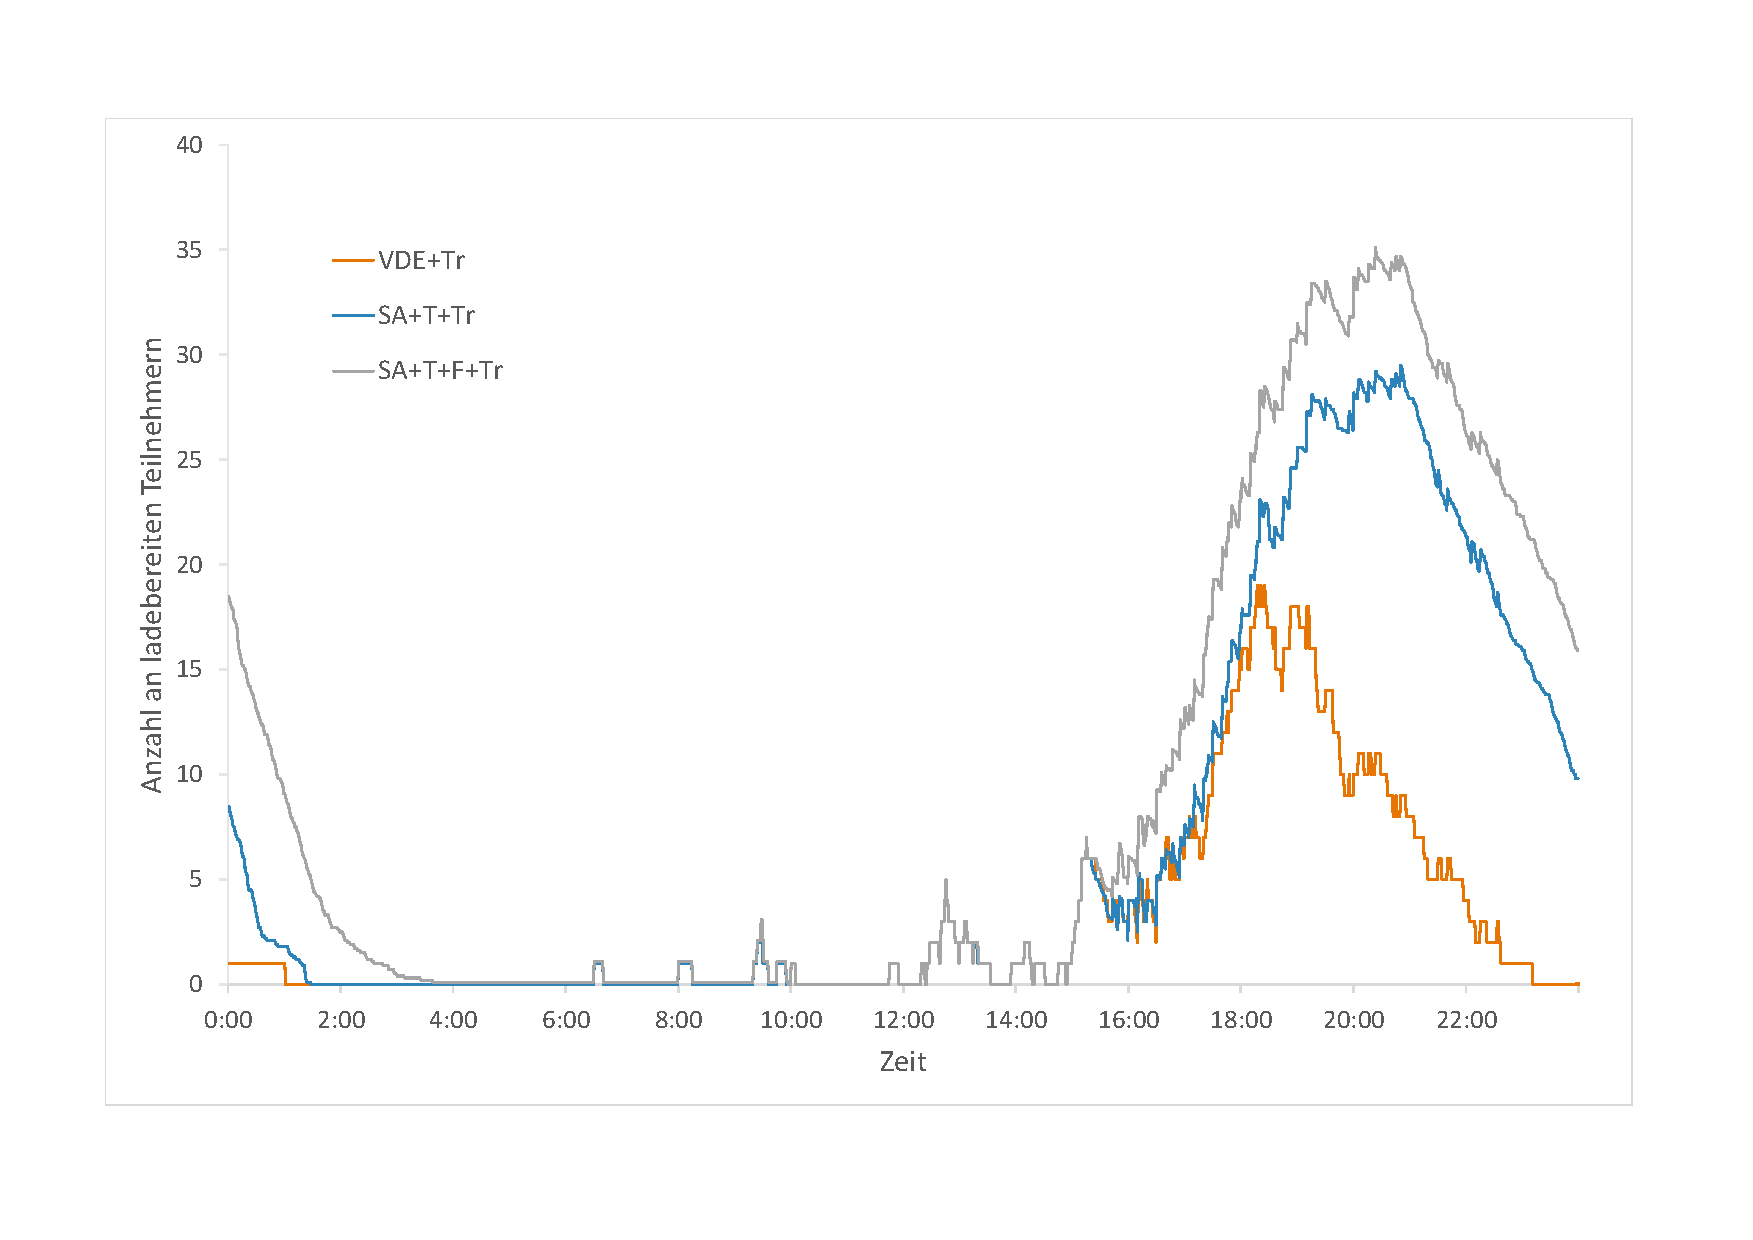
\includegraphics[scale=0.45]{img/mitTrafo/Teilnehmer_bereit.pdf}
        \subcaption{Anzahl der ladendbereiten Teilnehmer über den Verlauf eines Tages}
        \label{ABB_mT_teil2}
	\end{subfigure}
	\caption{Teilnehmerzahlen bei Verwendung von VDE+Tr, SA+T+Tr und SA+T+F+Tr}
\end{figure}
Abbildung \ref{ABB_mT_Teil1} zeigt die Anzahlen der ladebereiten Teilnehmer und Abbildung \ref{ABB_mT_teil2} zeigt die Anzahlen der ladenden Teilnehmer. Hier zeigen sich Unterschiede, welche bisher nicht ersichtlich waren. Durch die Limitierung der Ladeleistung durch den Transformatorkontroller, wird zwar die last am Transformator erfolgreich reduziert, allerdings baut sich auch die Menge an ladebereiten Fahrzeugen länger auf und langsamer wieder ab. Andererseits sind durch die reduzierte Leistungsaufnahme pro Teilnehmer mehr ladende Teilnehmer gleichzeitig möglich.
Beim Vergleich über die Transformatorlast, Die Spannungswerte und die Teilnehmerzahlen hinweg, zeigt sich dasselbe Ergebnis wie bereits beim Vergleich der Variante ohne den Transformatorkontroller. Der VDE-Kontroller ohne Erweiterungen liefert eine schlechtere Performanz ab als die beiden anderen Varianten, zusätzlich zu der Notwendigkeit der Überarbeitung der Technik um überhaupt auswertbare Ergebnisse zu liefern. Auch hier stellt sich die Variante, welche die Teilnehmerzahl und die Fahrzeugparameter verwendet, wieder als die Variante dar, welche die im aktuellen Vergleich besten Ergebnisse liefert. Der Abstand des VDE-Kontrollers zu den beiden Anderen setzt sich auch bei der Betrachtung der Norm DIN EN 50160 fort. Nur die beiden Varianten, welche Teile des Aloha Protokolls verwenden, sind in der Lage die Norm zu erfüllen.
Bei Betrachtung der Anzahl der möglichen Anzahl an Kollisionen zeigt sich zunächst ein anderes Bild als bisher.
\begin{table}[]
\centering
\begin{tabular}{l|l|l|l|}
\cline{2-4}
                                                                                       & Variante &             &             \\ \hline
\multicolumn{1}{|l|}{}                                                                 & VDE      & SA+T+Tr     & SA+T+F+Tr   \\ \hline
\multicolumn{1}{|l|}{\begin{tabular}[c]{@{}l@{}}mögliche \\ Situationen\end{tabular}}  & 5964.0     & 6589.3 ($\pm$ 1.6~\%) & 7077.0 ($\pm$ 4.3~\%) \\ \hline
\multicolumn{1}{|l|}{\begin{tabular}[c]{@{}l@{}}Anzahl an \\ Wartezeiten\end{tabular}} & 0        & 3084.0 ($\pm$ 0.7~\%)   & 2482.0 ($\pm$ 2.5~\%) \\ \hline
\end{tabular}
\caption{Anzahl der möglichen und tatsächlich aufgetreten Kollisionen bei den Methoden VDE+Tr, SA+T+Tr und SA+T+F+Tr}
\label{tab:my-table4}
\end{table}

Tabelle \ref{tab:my-table4} zeigt die Anzahl der möglichen und die Anzahl der aufgetretenen Kollisionen. Anders als es zu erwarten war nach den bisherigen Ergebnissen, ist es bei der Variante mit den Fahrzeugparametern in mehr Situationen möglich, dass eine Kollision auftritt als in einer anderen Variante. Betrachtet man allerdings nun die Anzahl der tatsächlich aufgetretenen Kollisionen zeigt sich wieder das zu erwartende Muster. Trotz deutlicher mehr Situationen in denen eine Kollision auftreten könnte, treten bei der Variante mit den Fahrzeugparametern die wenigsten Kollisionen auf.
\begin{figure}
	\begin{subfigure}{0.49\linewidth}
		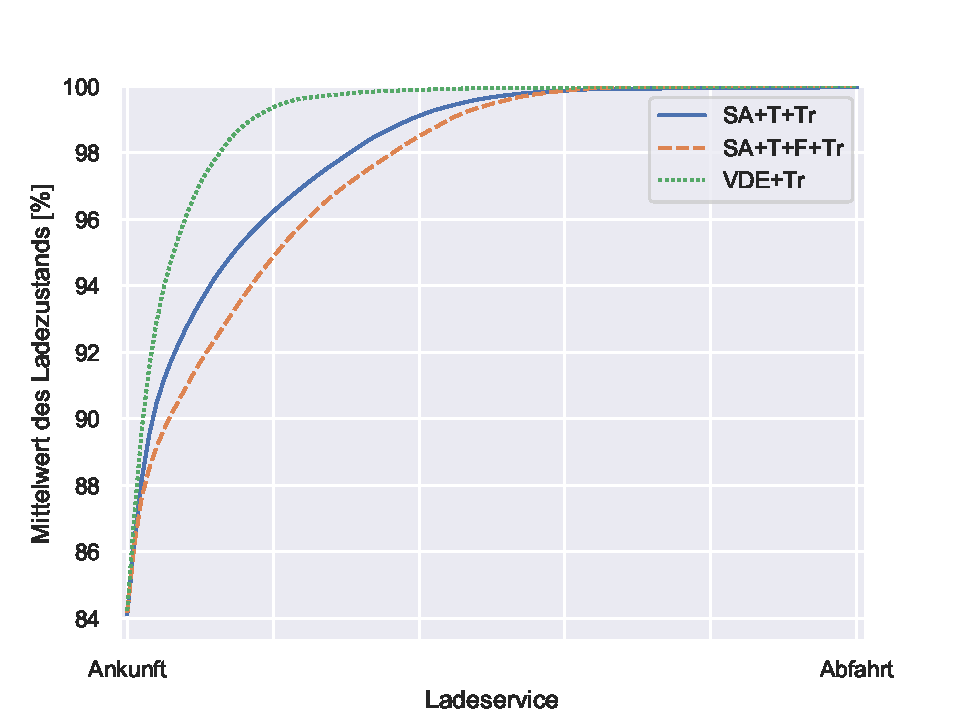
\includegraphics[width=\linewidth]{img/mitTrafo/SlottedAloha_participants_VDE_tau_trafo_13_soc_mean.pdf}
        \subcaption{Durchschnittlicher Ladezustand aller Elektrofahrzeuges über den Verlauf eines Ladeservices}
        \label{ABB_mt_SocMEAN}
	\end{subfigure}
	\begin{subfigure}{0.49\linewidth}
		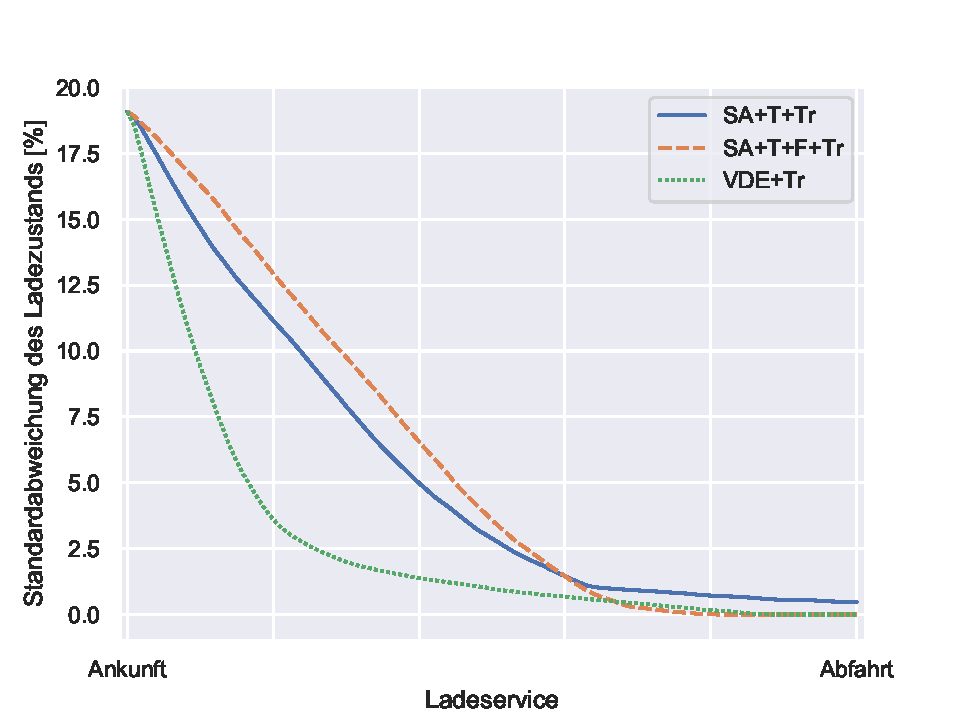
\includegraphics[width=\linewidth]{img/mitTrafo/SlottedAloha_participants_VDE_tau_trafo_13_soc_std.pdf}
        \subcaption{Durschschnittliche Standardabweichung des Ladezustandes aller Elektrofahrzeuges über den Verlauf eines Ladeservices}
        \label{ABB_mT_SocSTD}
	\end{subfigure}
	\caption{Durchschnittlicher Ladezustand mit Standardabweichung bei Verwendung von VDE+Tr, SA+T+Tr und SA+T+F+Tr}
\end{figure}
In Abbildung \ref{ABB_mt_SocMEAN} sind die jeweiligen mittleren Ladestände aller Fahrzeugen über den Verlauf der Ladeservice hinweg dargestellt, Abbildung \ref{ABB_mT_SocSTD} zeigt die zugehörige Standardabweichung. Abbildung \ref{ABB_mt_SocMEAN} zeigt einen ähnlichen Verlauf der Kurven, welche das Netzwerkprotokoll verwenden. Allerdings wird auch ersichtlich, dass die Variante, welche nur die Teilnehmerzahl verwendet, nicht dazu in der Lage ist alle abgeschlossenen Ladeservice auch erfolgreich abzuschließen, da die Standardabweichung nicht bis auf null zurückgeht. 
\begin{figure}[htb]
\centering
	\includegraphics[scale=0.45]{img/mitTrafo/SlottedAloha_participants_VDE_tau_trafo_13_qoe.pdf}
	\caption{Durchschnittlicher Qualitätserfahrungs Fairness Index aller Elektrofahrzeuges über den Verlauf eines Ladeservices bei Verwendung von VDE+Tr, SA+T+Tr und SA+T+F+Tr}
	\label{Abb_mT_Fairness}
\end{figure}
Abbildung \ref{Abb_mT_Fairness} zeigt die mittlere Fairness aller Fahrzeuge über den Verlauf der Ladeservice hinweg mit der zugehörigen Standardabweichung für alle drei betrachteten Varianten. Auch hier zeigt sich wieder der Nachteil der Variante mit dem Netzwerkprotokoll, welche nur die Teilnehmerzahl verwendet, da nicht alle Ladeservice erfolgreich waren, erreicht auch die Fairness nicht dem maximal möglichen Wert. Wie bereits beim mittleren Ladestand und der dazugehörigen Standardabweichung liefert der VDE-Kontroller teils bessere Ergebnisse als die beiden anderen Varianten, dies wird allerdings aufgrund der Ergebnisse bei der Transformatorlast und den Spannungswerten relativiert, da der VDE-Kontroller dort im Vergleich das unzureichenste Ergebnis erbracht hat. Der Unterschied zwischen den Kurven von SA+T+Tr und SA+T+F+Tr hat sich im Vergleich zu den Ergebnissen ohne Transformatorkontroller vergrößert auch der Verlauf der Kurven an sich wurde flacher. Dieser Unterschied geht zurück auf das Mehr an Wartezeiten die aufgrund des Transformatorkontrollers berechnet werden und so für stärkere zeitliche Verteilung der Teilnehmer sorgt. Diese stärkere zeitliche Verteilung zögert auch das Erreichen eines hohen Ladestandes hinaus, da mehr Zeit des Ladeservices mit Warten verbracht wird. So zeigt sich erneut der Unterschied in der Bestimmung der Wartezeiten wenn nur die Teilnehmerzahl berücksichtigt wird, werden bereits kleiner Intervalle bestimmt aus denen dann auch kürzere Wartezeiten bestimmt werden.\\ 


Insgesamt ergibt sich bei der Betrachtung aller betrachteten Messwerte der Ergebnisse, wenn der Transformatorkontroller verwendet wird dasselbe Bild als, wenn er nicht verwendet wird. Die beiden Varianten, welche das Slotted Aloha Netzwerkprotokoll mitverwenden, liefern vor allem bei der Transformatorlast und den Spannungswerten bessere Ergebnisse.  Allerdings ist nur bei der Verwendung des Transformatorkontrollers, da das gesetzte Ziel der Regulierung der Transformatorlast erreicht worden, nur die Verwendung eines Spannungskontrollers hat nicht zum Erreichen dieses Ziels ausgereicht.
